\documentclass[../document.tex]{subfiles}
\begin{document}
\section{Implementation}

\subsection{Tools}
The most important tools and libraries used in our work were:

\begin{itemize}
	\item ROS Melodic
	\item Numpy
	\item Matplotlib
	\item Pandas
	\item OpenCV
	\item PyTorch
	\item FastAI
	\item imgaug
	\item Blender
\end{itemize}
The framework was entirely developed on Ubuntu 18.10 with Python 3.6.

\subsubsection{ROS Melodic}
The Robot Operating System (ROS) \cite{ROS} is a flexible framework for writing robot software. It is \emph{de facto} the industry and research standard framework for robotics due to its simple yes effective inferface that facilitates the task of creating robust and complex robot behavior regardless of the platforms. ROS work by generate a peer-to-peer connection where each \emph{node} is to communicate between the others by exposing sockets endpoints to stream data called \emph{topics}. 

Each \emph{node} can subscribe to received the incoming messages or publish new data on a specific \emph{topic}. In our case, \emph{Krock} exposes different topics, for example \texttt{/pose}, in which we can subscribe in order to get the real time informations about the state of the robot.
Unfortunately, ROS does not natively support Python3, so we had to compile it by hand. Since it was not difficult and time consuming operation we decided to share the ready-to-go binaries as docker image. \todo{where should I place the link to docker}

\subsubsection{Numpy}
Numpy is a fundamental packages for any scientific use. Thanks to its powerful N-dimensional array object with the sophisticated broadcasting functions, it is possible to express efficiently any matrix operation. We utilised \emph{Numpy} manipulate matrices in an expressive and efficient way.
\todo[inline]{scrape some text from the previous section}

\subsubsection{Matplotlib}
Matplotlib is a widely used Python 2D plotting library which generates high  quality figures in a variety of hardcopy formats and interactive environments across platforms. It provides a similar functional interface to MATLAB and a deep ability to customise every region of the figure. Almost every figures made in this report were produced using Matplotlib.
It is worth citing \emph{seaborn} a data visualization library that we inglobate in our work-flow. It is based on Matplotlib and it provides a high-level interface for drawing attractive and informative statistical graphics.
\subsubsection{Pandas}

Pandas is a Python library providing fast, flexible, and expressive data structures in a tabular form. It aims to be the fundamental high-level building block for doing practical, real world data analysis in Python. Today, it one of the most flexible open source data manipulation tool available. Pandas is well suited for many different kinds of data such as handle tabular data with heterogeneously-typed columns, similar to SQL table or Excel spreadsheet, time series and matrices. It provides to two primary data structures, \texttt{Series} and \texttt{DataFrame} for representing 1 dimensional and 2 dimensional  data respectively.  

Generally, pandas does not scale well and it is mostly used to handle small dataset while relegating \"big data\" to other frameworks such as Spark or Hadoop. We used Pandas to store the results from the simulator and inside a Thread Queue to parse each \emph{.csv} file efficiently. 
\subsubsection{OpenCV}
Open Source Computer Vision Library, OpenCV, is an open source computer vision library with a rich collection of highly optimized algorithms. It includes classic and state-of-the-art computer vision and machine learning methods applied in a wide array of tasks, such as object detection and face recognition.
 With a huge community of more than fourtyseven thousand people, the library is a perfect choice to handle image data. 
In our framework, OpenCV is used to pre and post-process the heightmaps and the patches.
\subsubsection{PyTorch}
\emph{PyTorch} is Python open source deep learning framework. It allows Tensor computation (like NumPy) with strong GPU acceleration and Deep neural networks built on a tape-based autograd system. Due to its \emph{Python-first} philosophy it has a deep integration into Python allows popular libraries and packages to be used, such as \emph{OpenCV} or \emph{Pillow}.  

Due to its simply yet expressive and beautiful object oriented API it has been adopted be a huge number of researches and enthusiastics all around the world creating a flourishing community. 
Its main advantages over other mainstream frameworks such as TensorFlow \todo{cite TF} are a cleaner API structure, better debugging, code shareability and enormous number of high quality packages. All the neural network proposed in this project are built using Pytorch.

\subsubsection{FastAI}
FastAI is  library based on PyTorch that simplifies fast and accurate neural nets training using modern best practices. It provides a high-level API to create train, evaluate and test deep learning models on any type of dataset.

\subsubsection{imgaug}
Image augmentation (imgaug) is a python library to perform image augmenting operations on images. It provides a variety of methodologies, such as affine transformations, perspective transformations, contrast changes and gaussian noise, to build sophisticated pipelines. It supports images,  heatmaps, segmentation maps, masks, keypoints/landmarks, bounding boxes, polygons and line strings.

\subsubsection{Blender}
Blender is the free and open source 3D creation suite. It supports the entirety of the 3D pipeline modeling, rigging, animation, simulation, rendering, compositing and motion tracking, even video editing and game creation. We used Blender to render some of the 3D terrain used to evaluate the  trained model.

\subsection{Data Gathering}
\subsubsection{Heightmap generation}
An heightmap is a 2D array, an image, where each pixel's value represent the terrain height.

\begin{figure}[H]
    \centering
        \begin{subfigure}[b]{0.45\textwidth}
            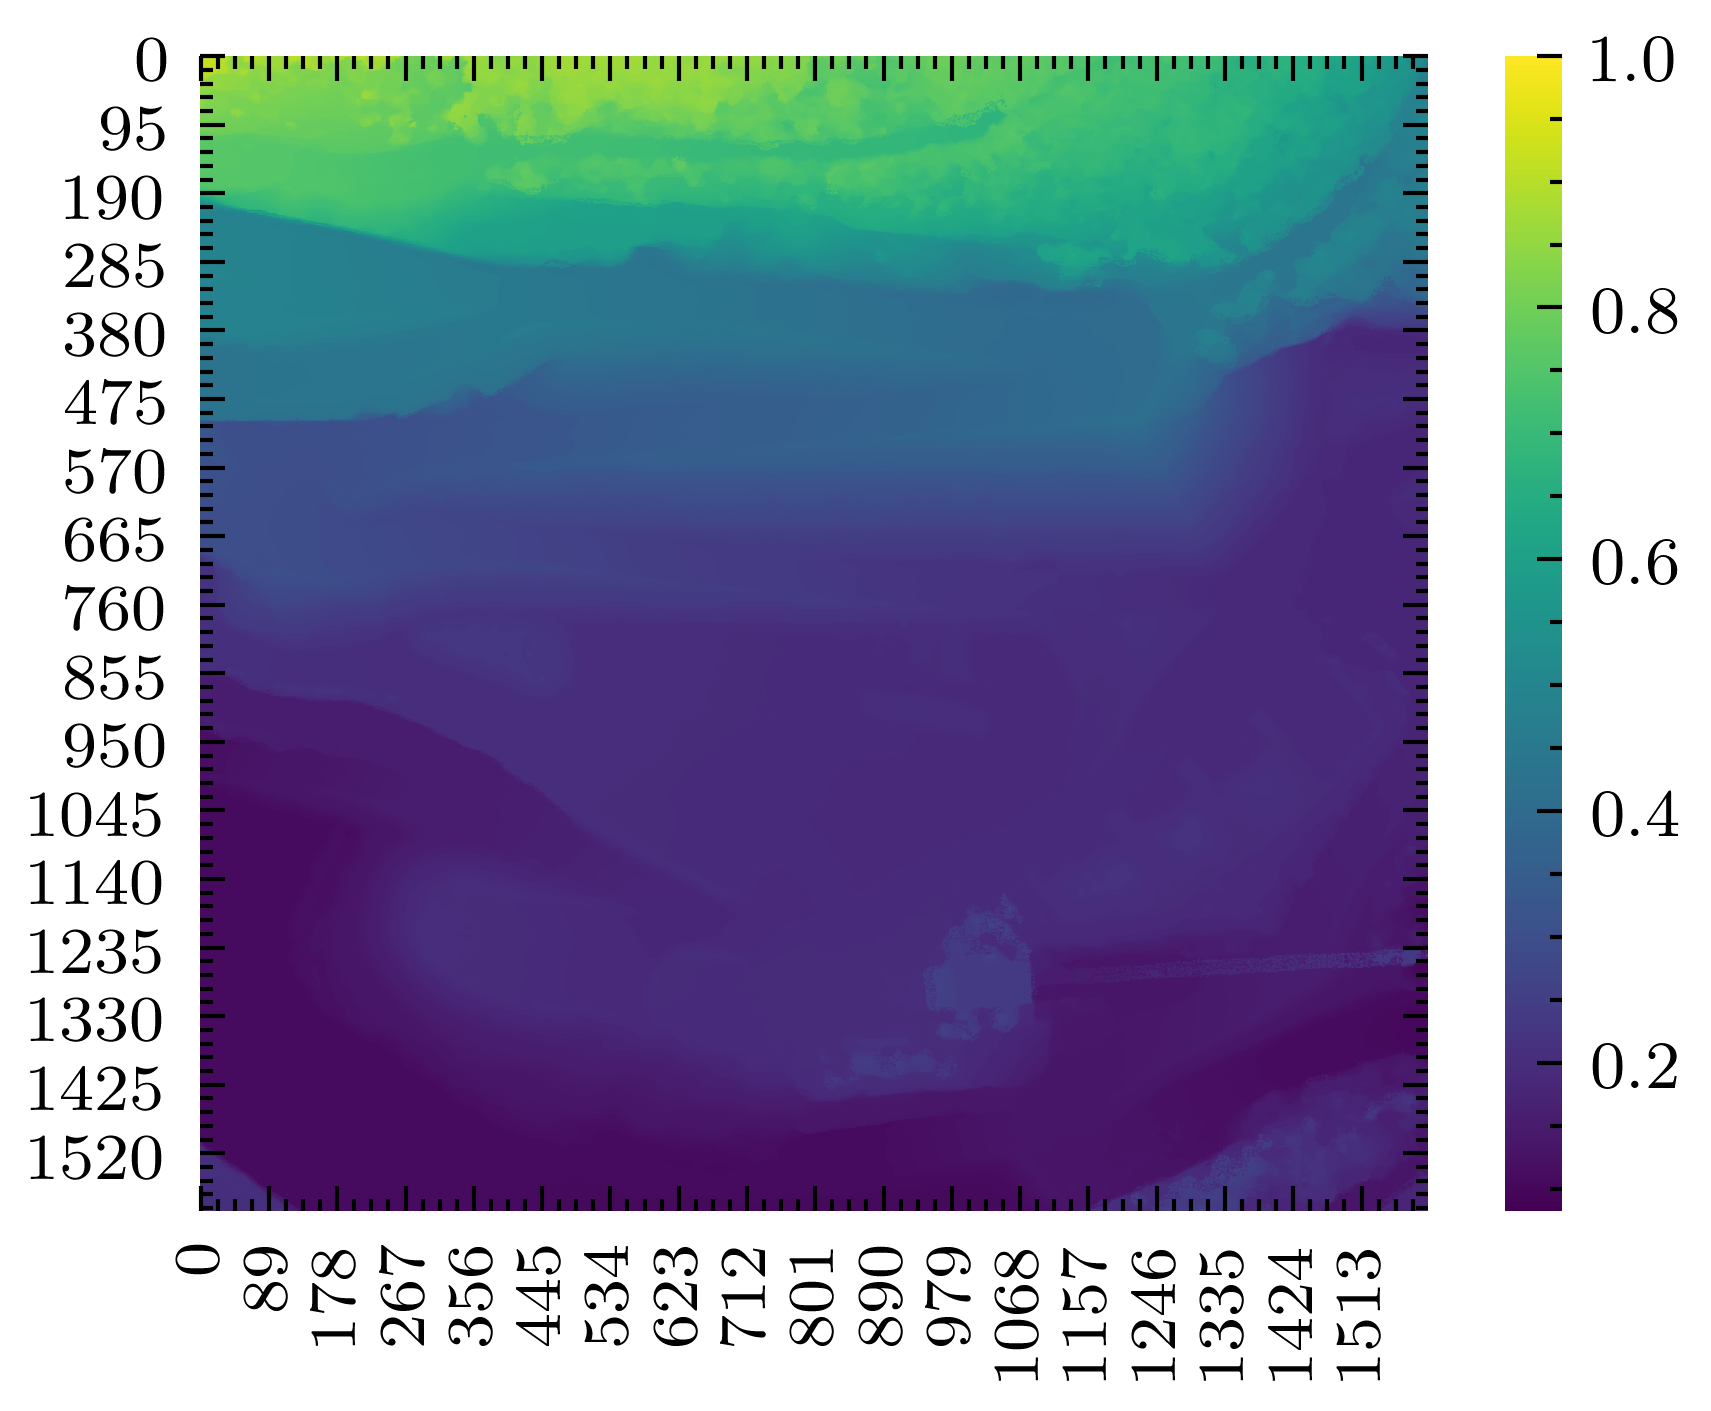
\includegraphics[width=\textwidth]{../img/hm/querry-big-10.png}
            \caption{\emph{Quarry} heightmap}
        \end{subfigure}
        \begin{subfigure}[b]{0.45\linewidth}
            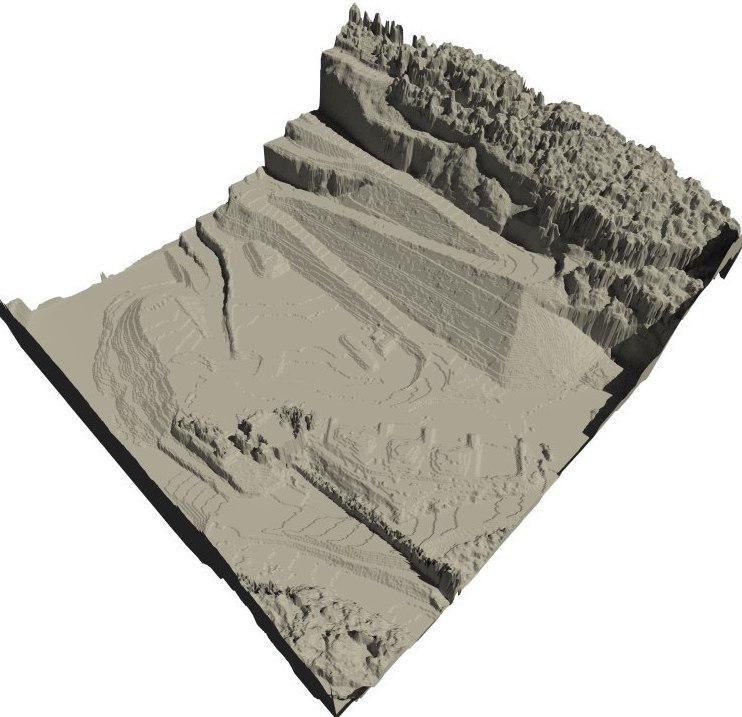
\includegraphics[width=\textwidth]{../img/quarry-rendered.png}
            \caption{\emph{Quarry} rendered}
            \end{subfigure}    
    \end{figure}
We generate fifteen terrain using random 2D simplex noise \cite{simplex}, a variant of Perlin noise \cite{perlin}, a widely used technique in terrain generation litterature.
\todo[inline]{3d rendered heightmap from Blender should visualize better the idea}
\begin{figure}[H]
    \centering
        \begin{subfigure}[b]{0.45\textwidth}
            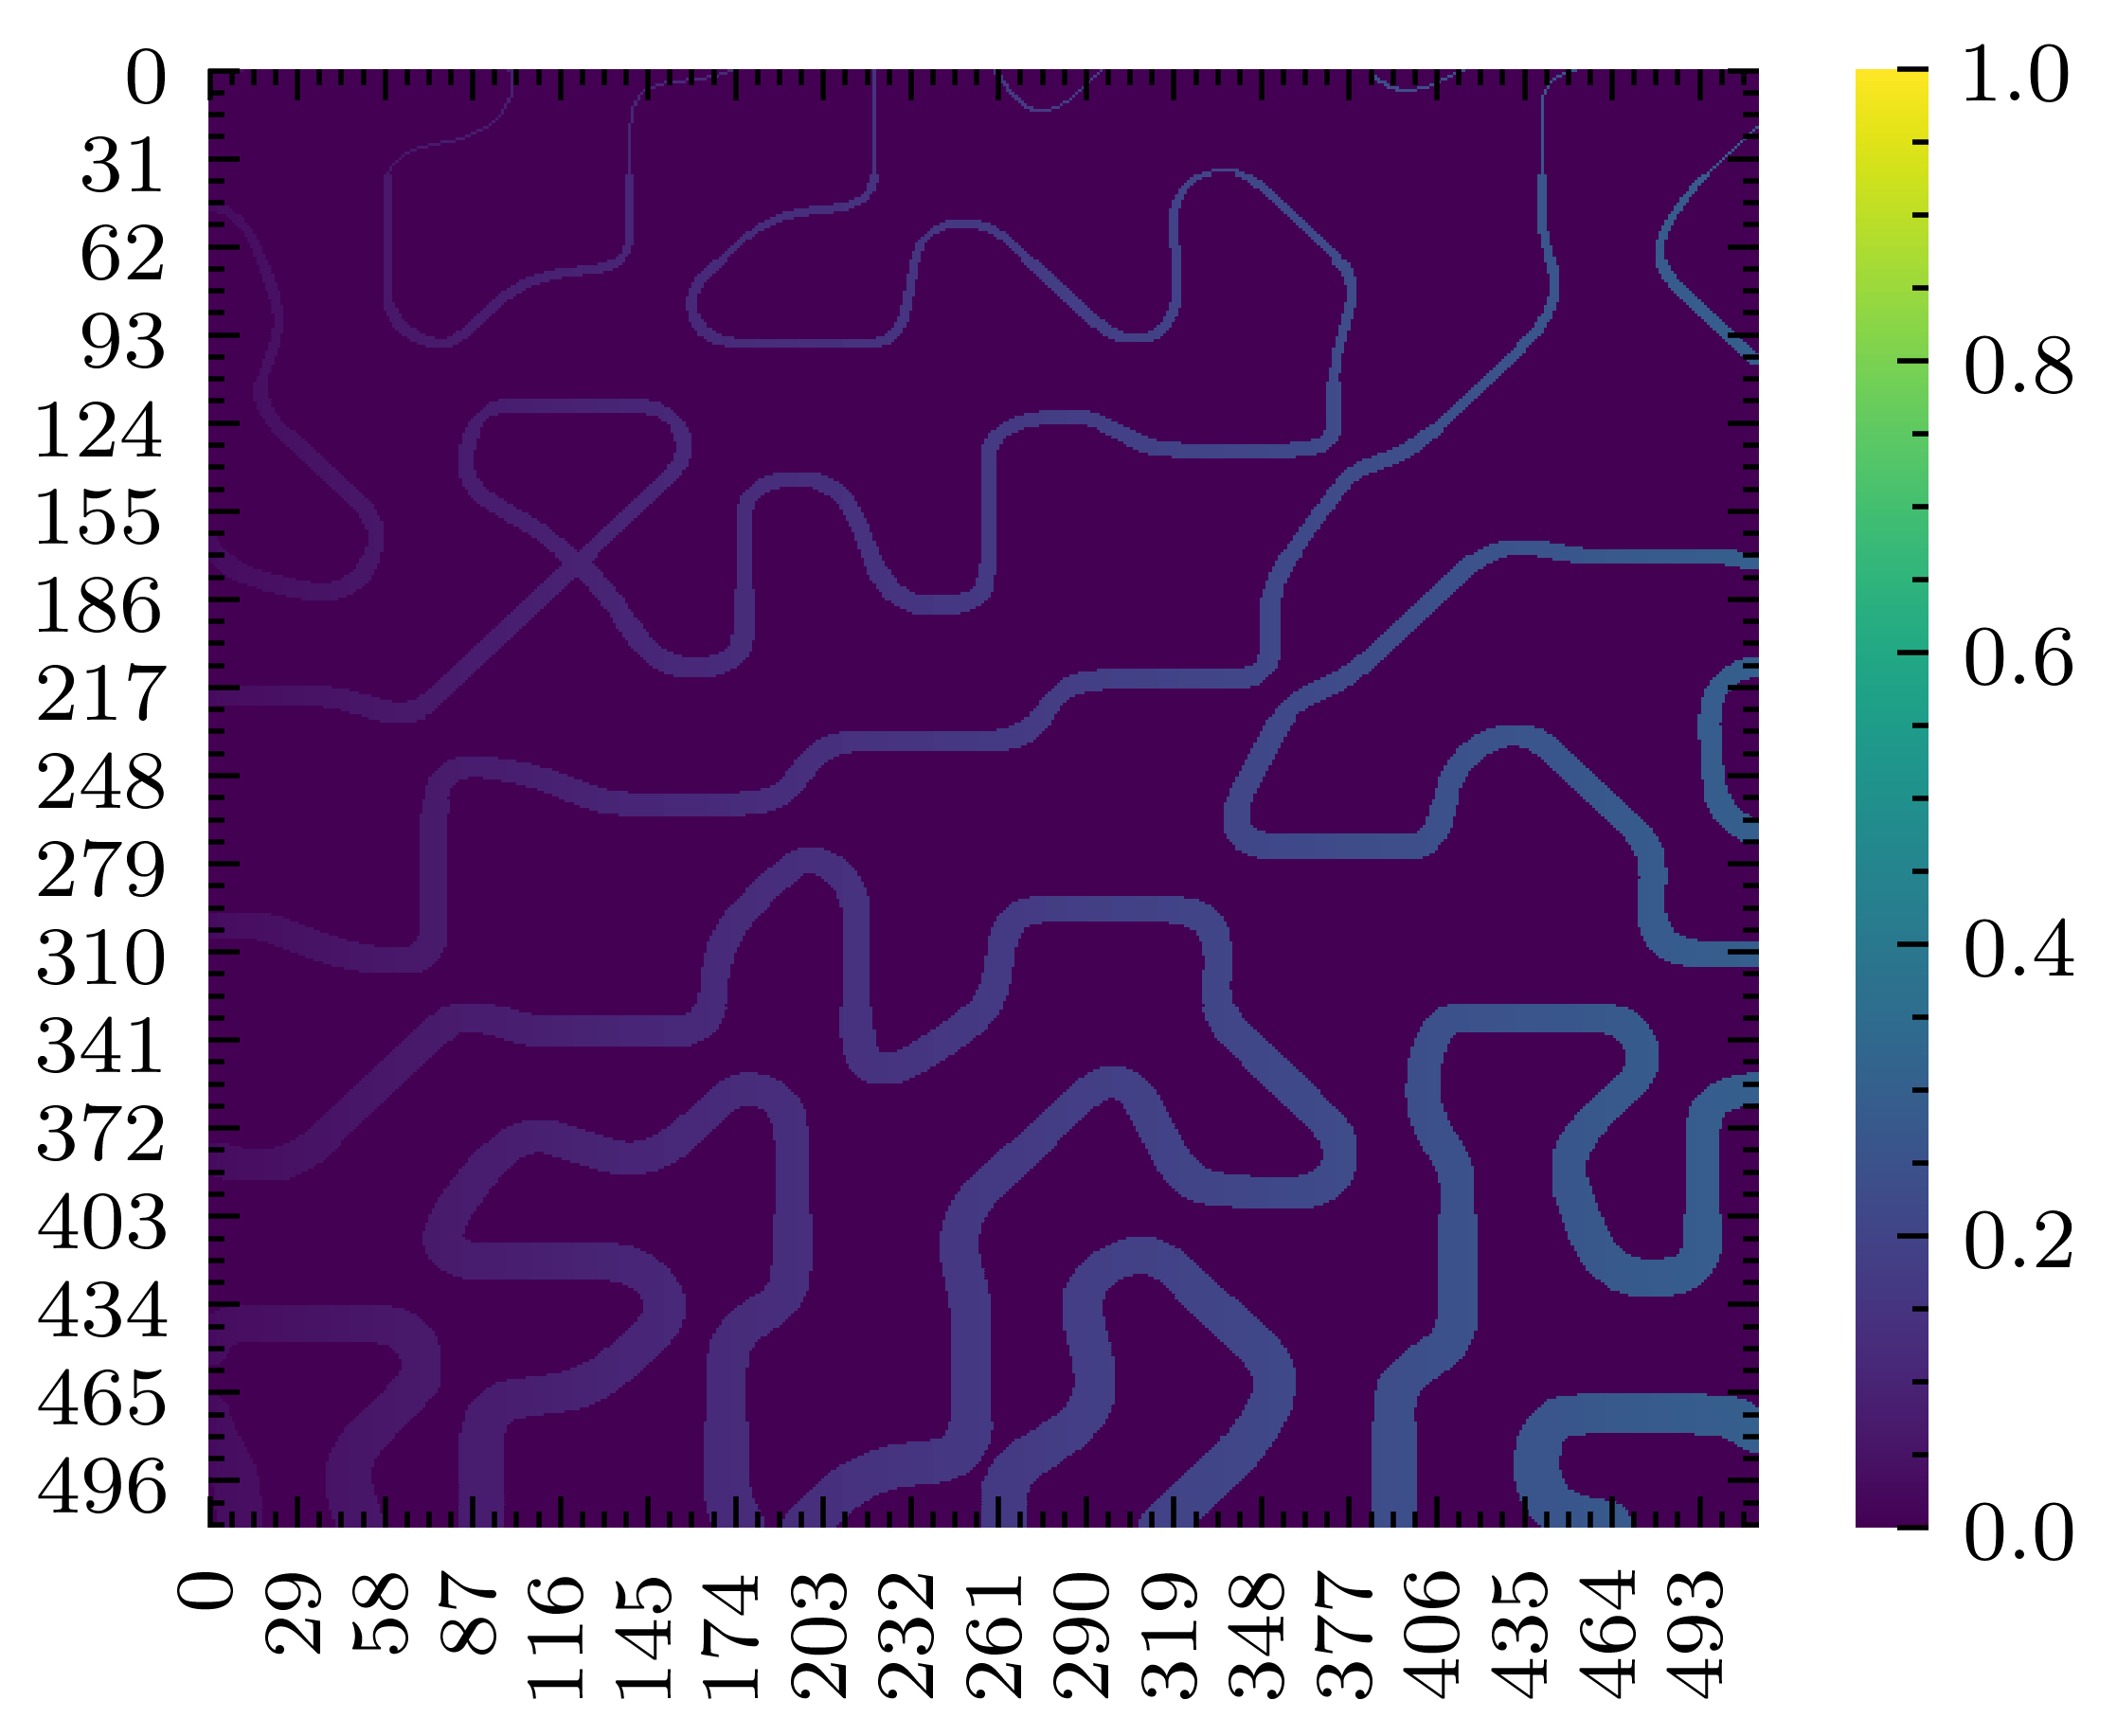
\includegraphics[width=\textwidth]{../img/hm/bars1.png}
            \caption{\emph{bars1}}
        \end{subfigure}
        \begin{subfigure}[b]{0.45\linewidth}
            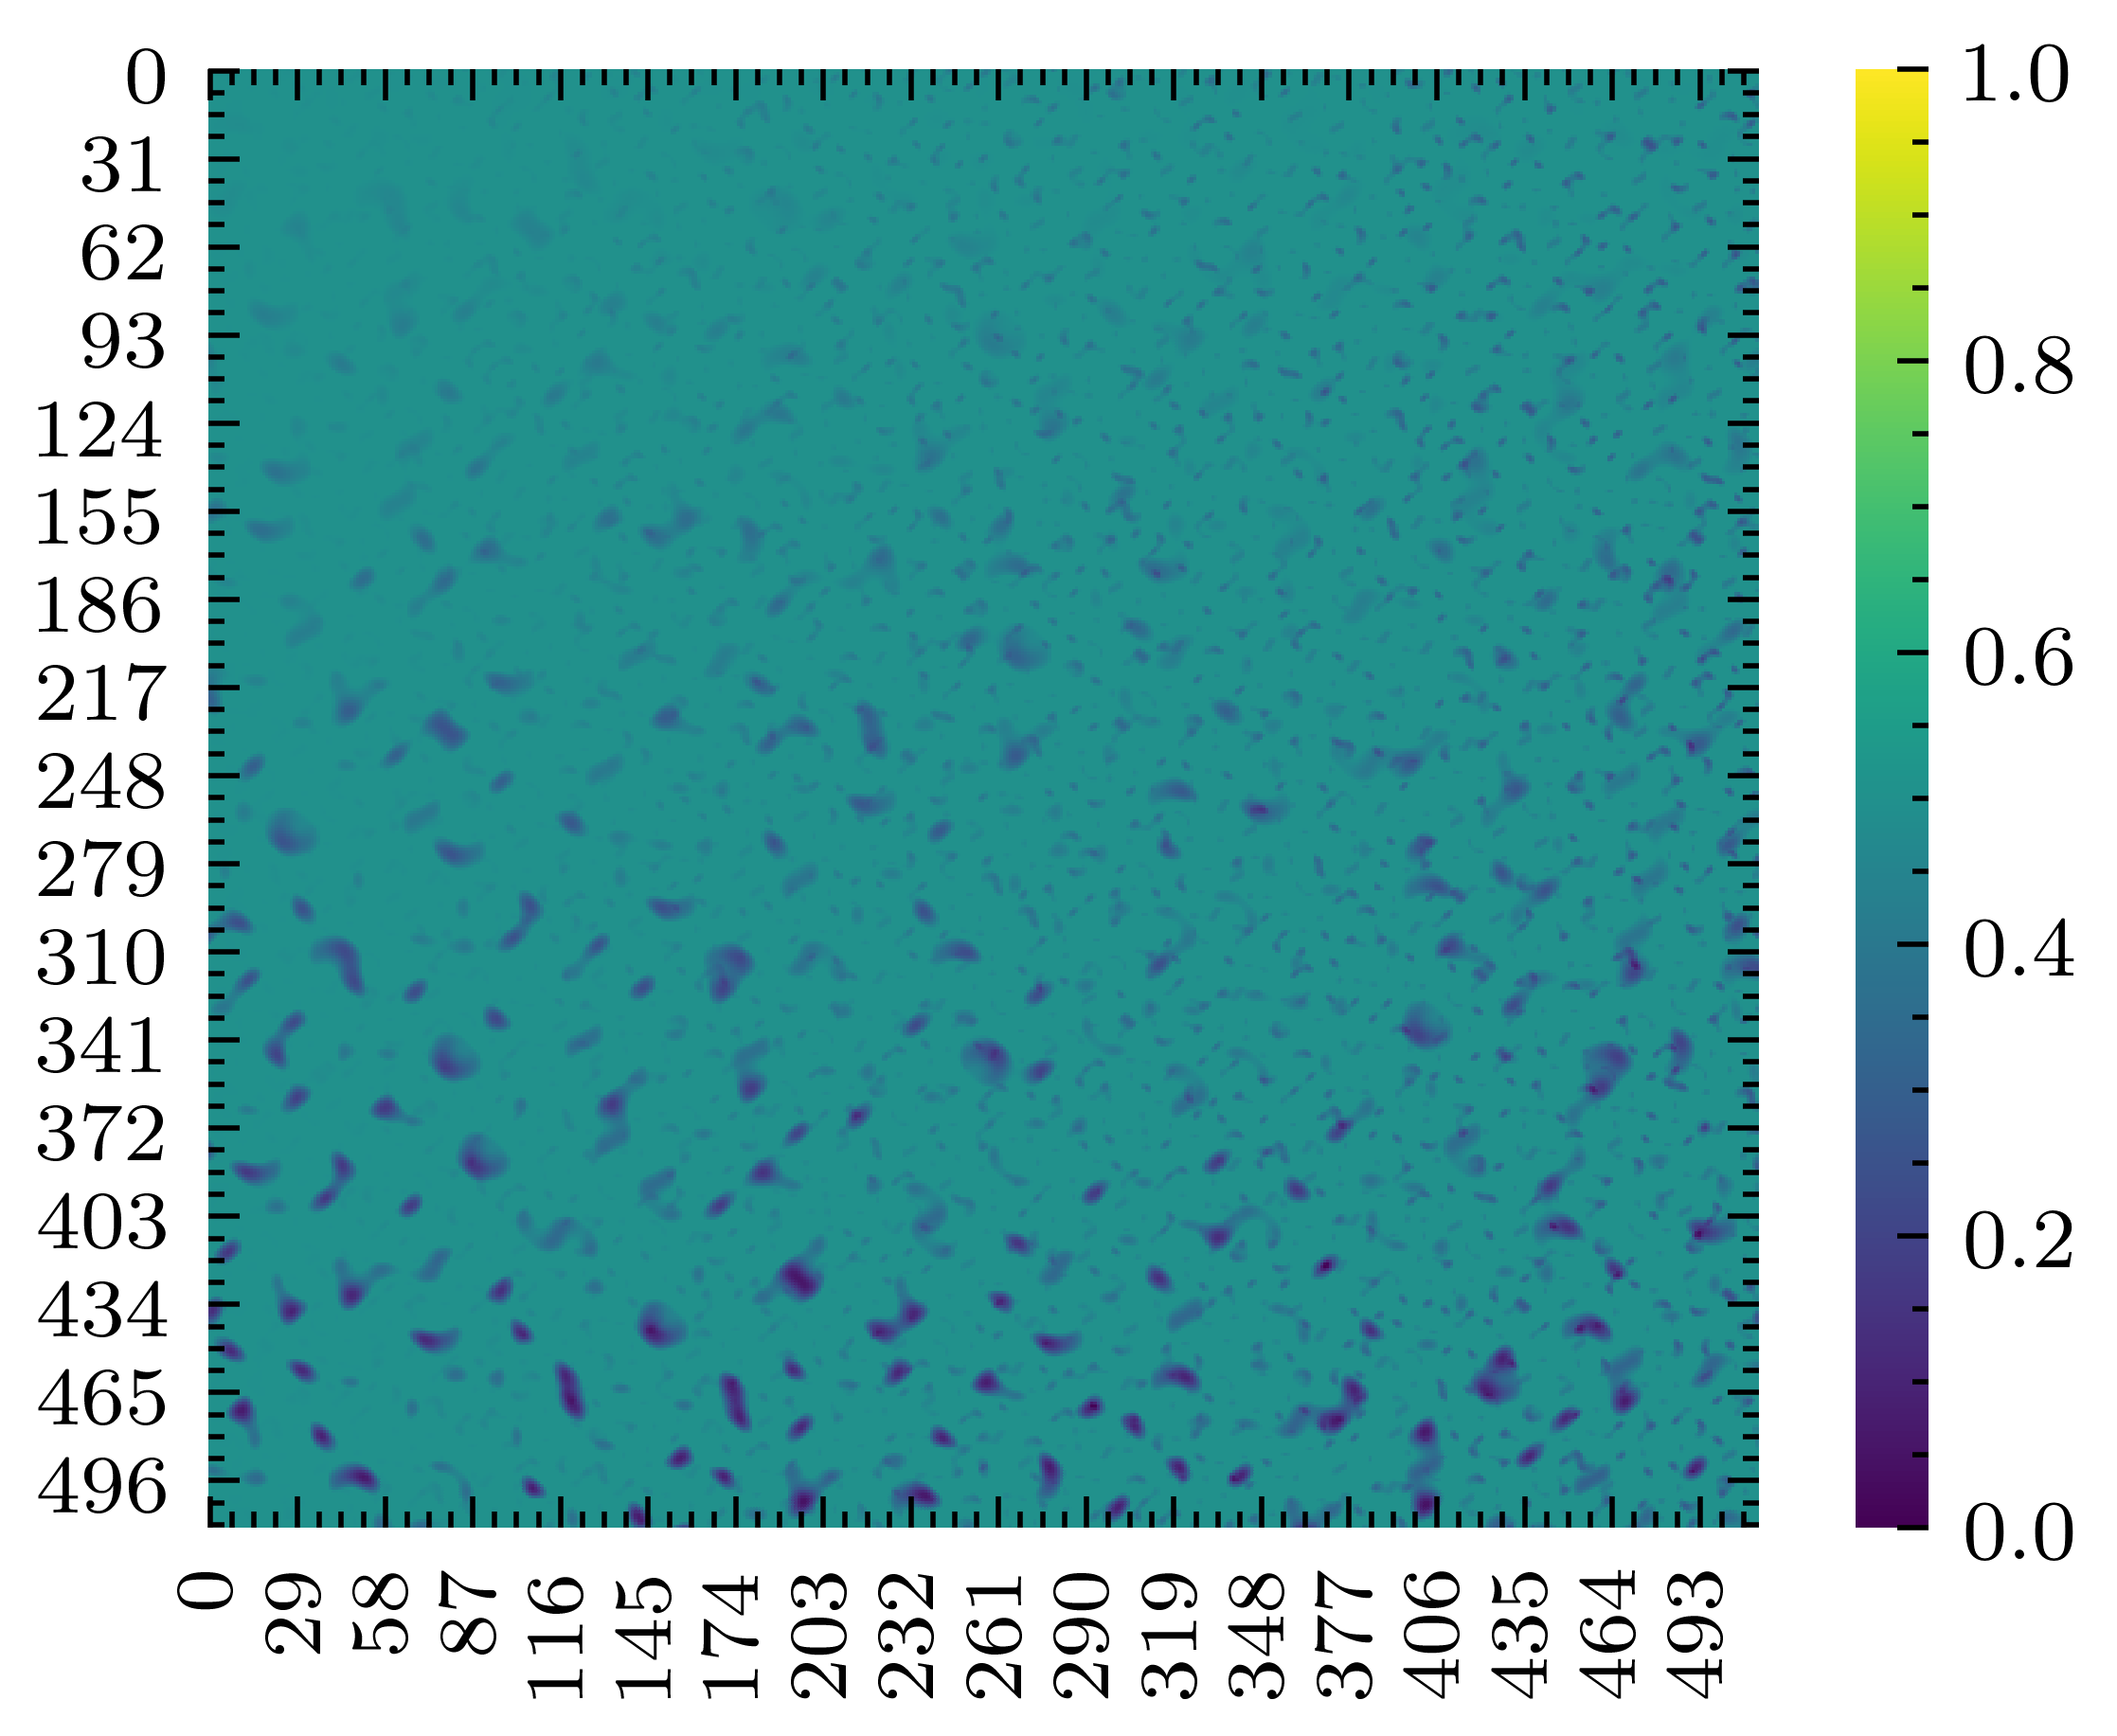
\includegraphics[width=\textwidth]{../img/hm/holes1.png}
            \caption{\emph{holes1}}
            \end{subfigure}    
          \begin{subfigure}[b]{0.45\textwidth}
            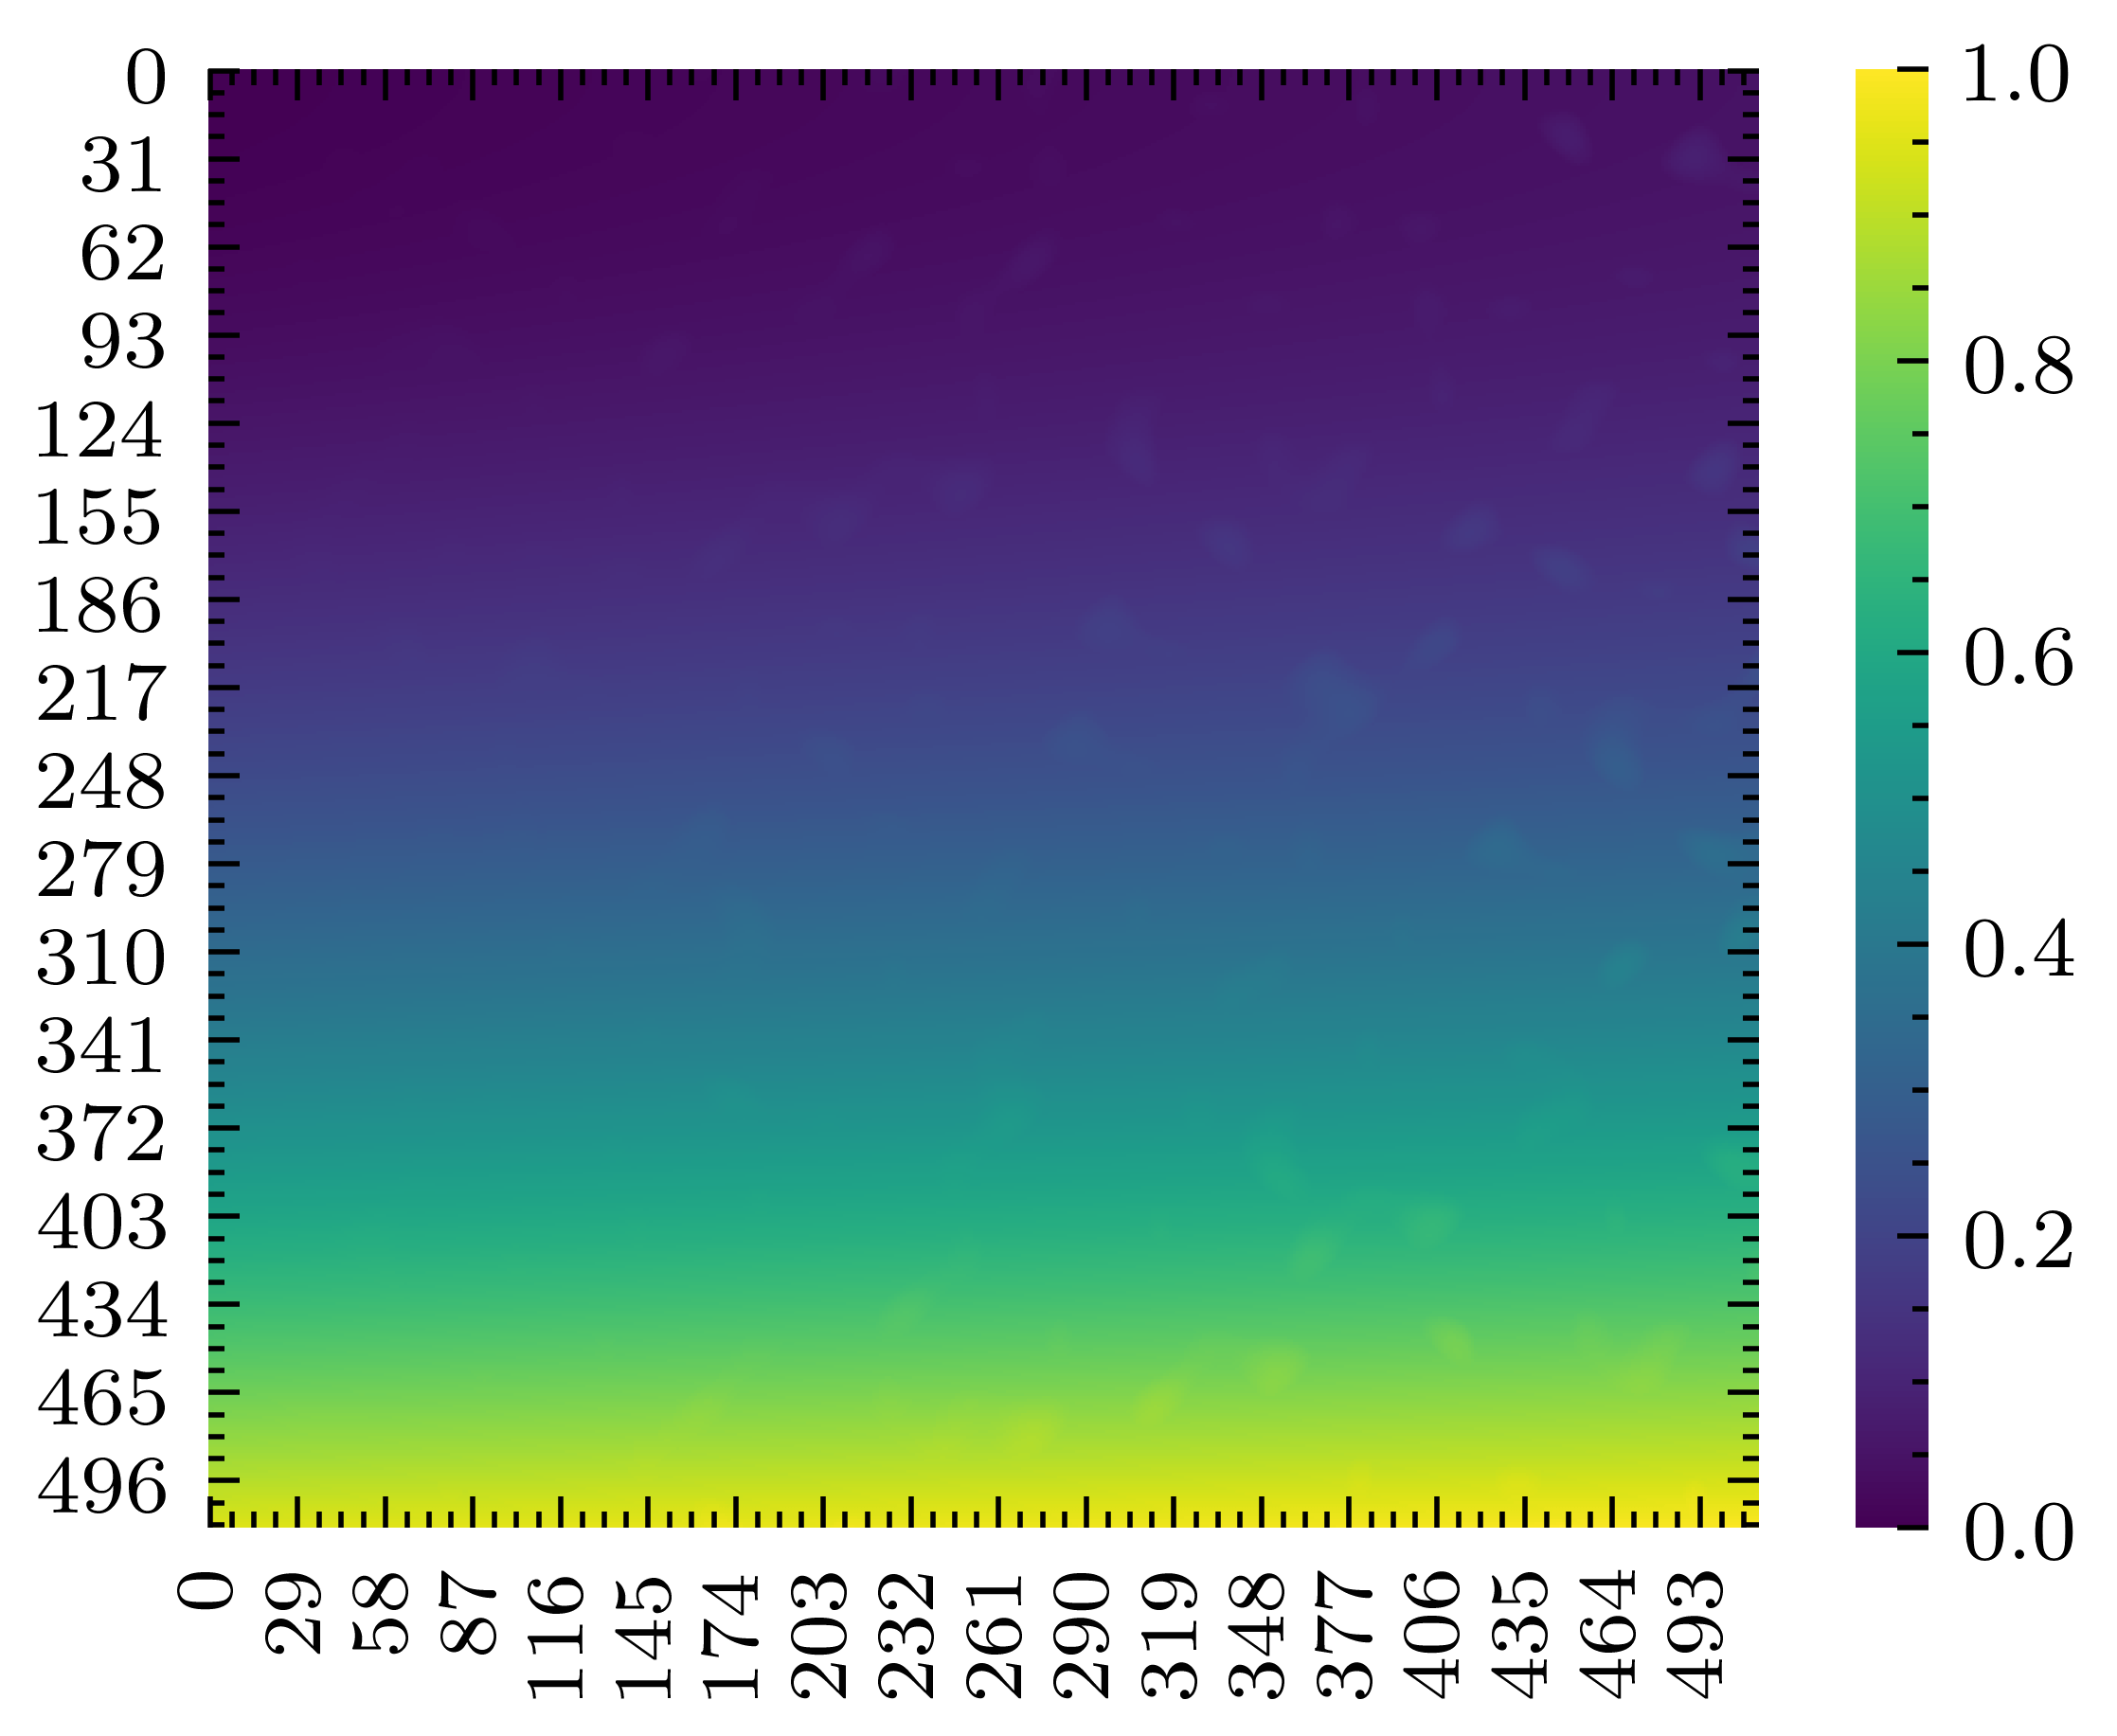
\includegraphics[width=\textwidth]{../img/hm/slope_rocks1.png}
            \caption{\emph{slope\_rocks1}}
        \end{subfigure}    
        \begin{subfigure}[b]{0.45\textwidth}
            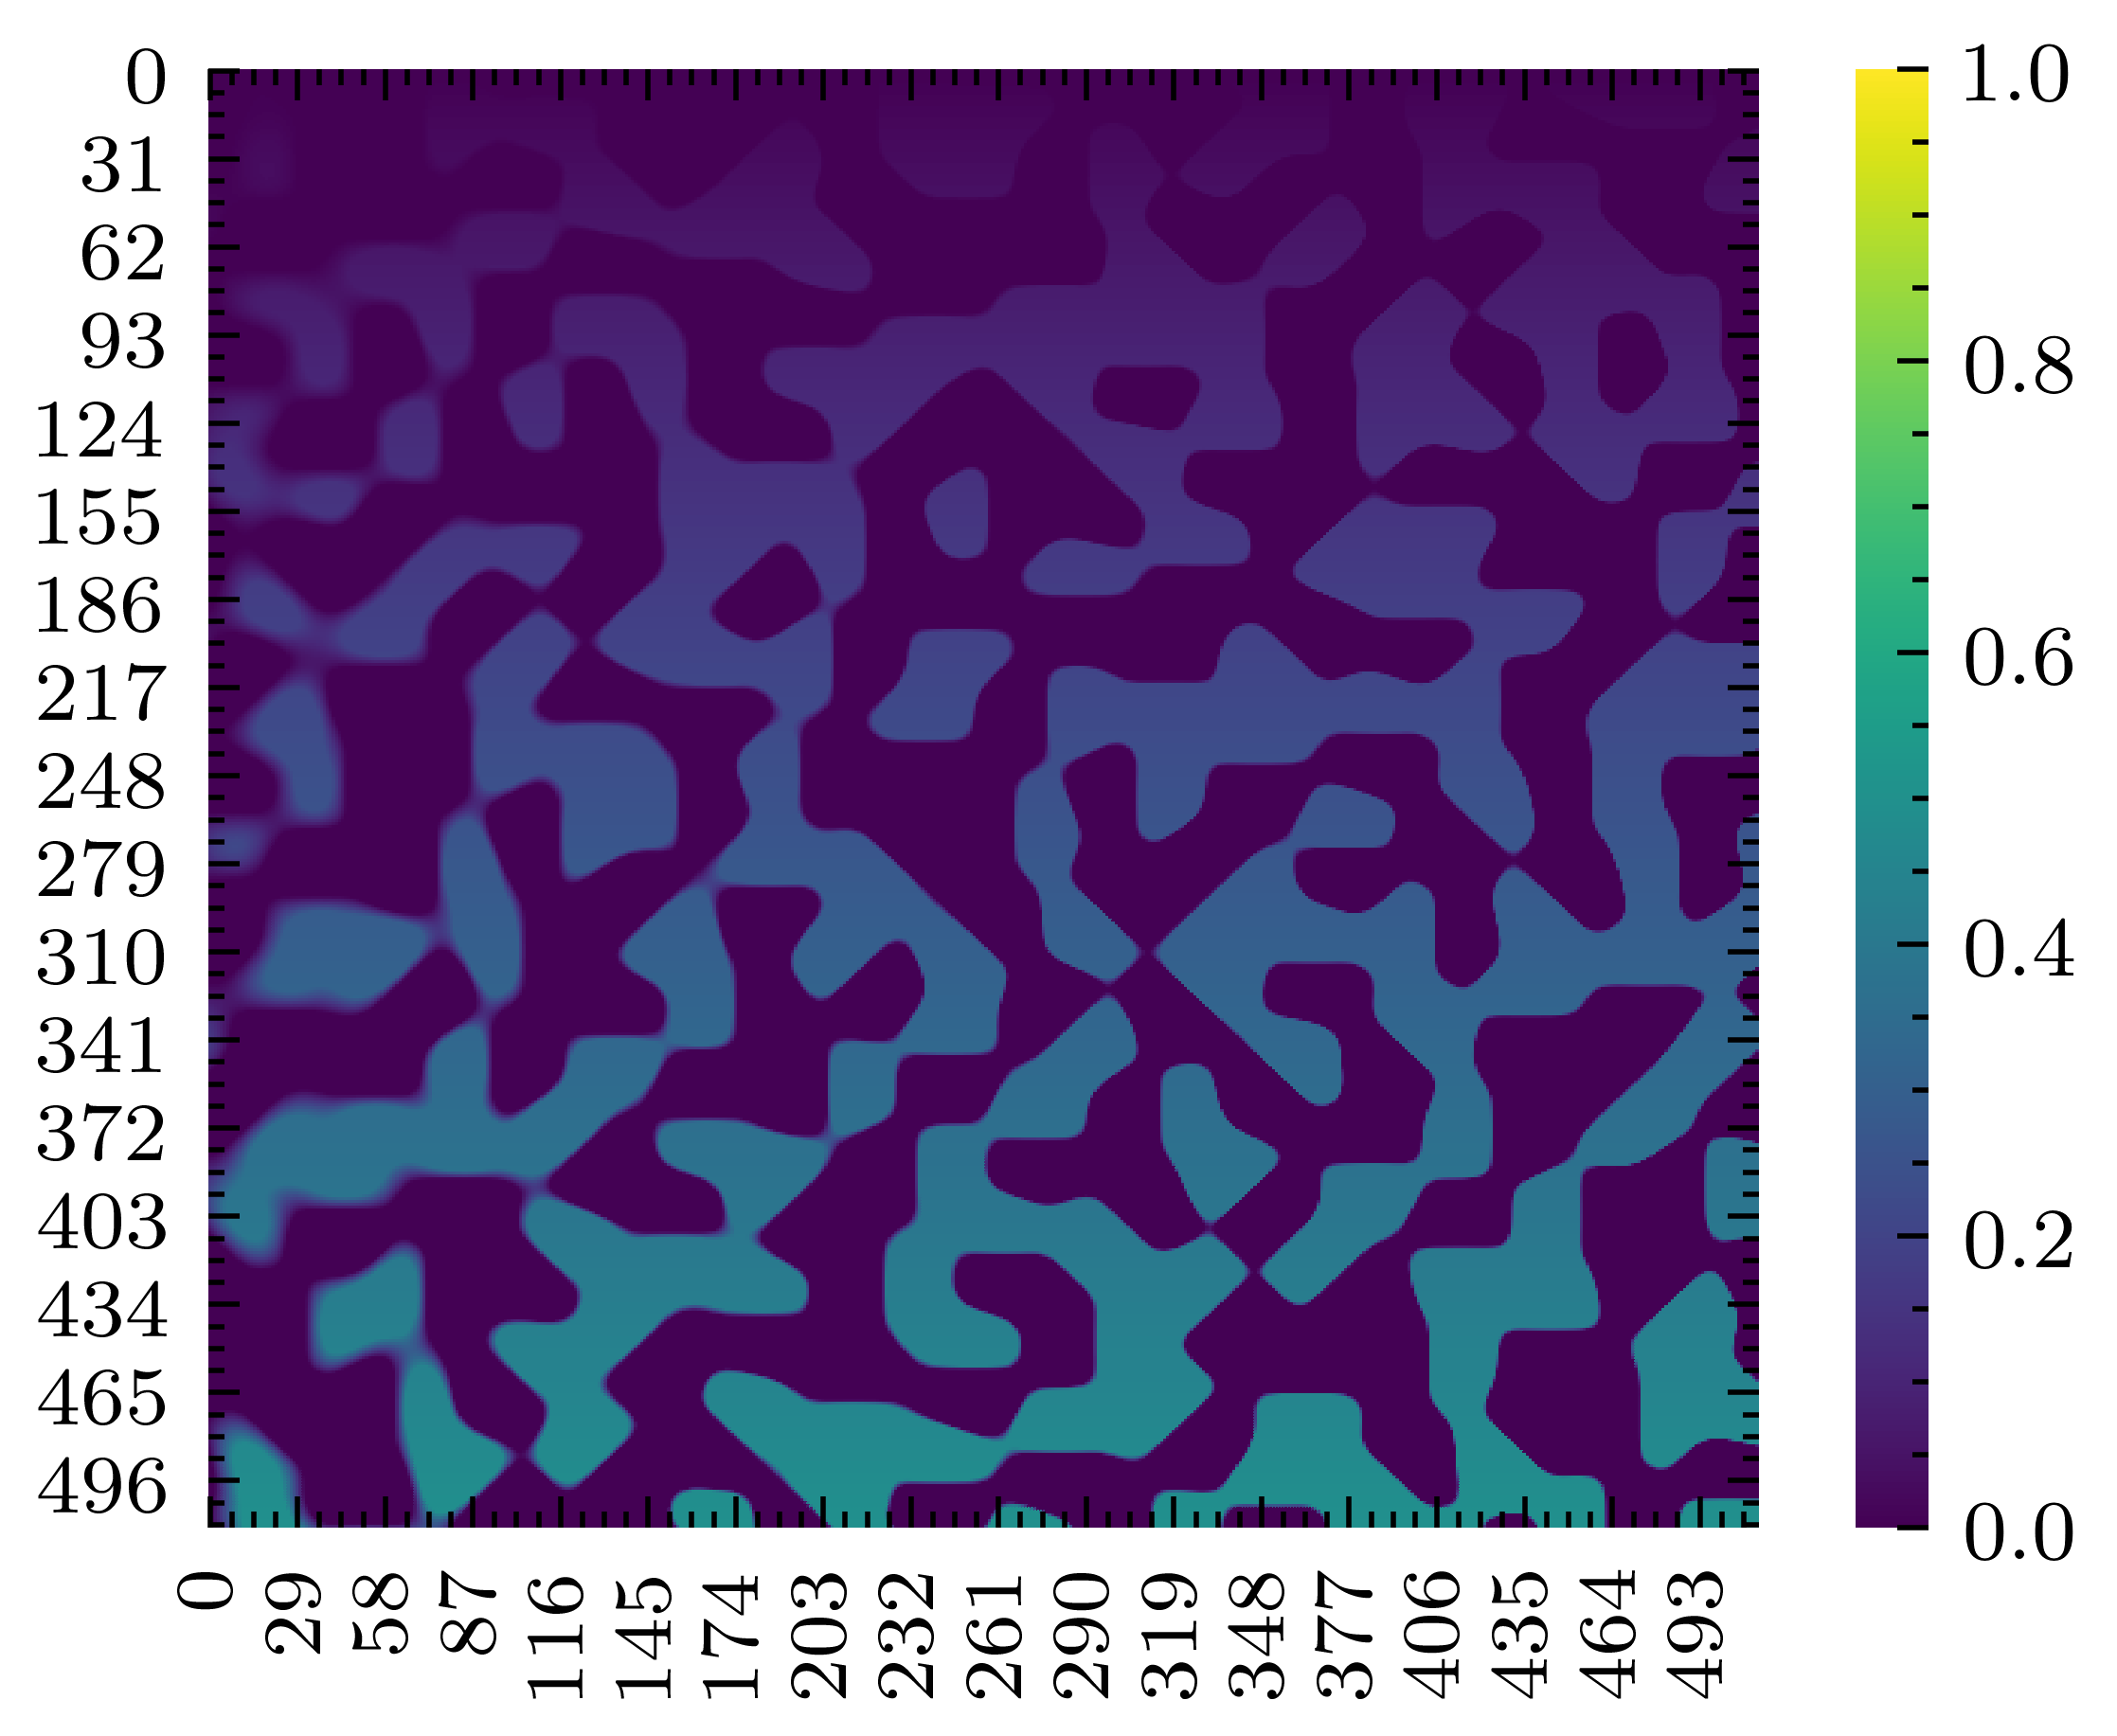
\includegraphics[width=\textwidth]{../img/hm/steps1.png}
            \caption{\emph{steps1}}
        \end{subfigure}    
    \label{fig: heightmaps}
    \caption{Some of the synthetic heightmaps}
\end{figure}
\subsubsection{Simulator}
We used Webots to simulate \emph{Krock} behaviour on the previously generated heightmap. The robot controlled was implemented by EPFL \todo{cite them?} and handed to IDSIA \todo{cite?}. The controller implements a ROS' node to publish \emph{Krock} status including its pose at a rate of $250hz$. We decide to reduce it $50hz$ by using ROS build it \texttt{throttle} command. 
To load the map into the simulator we had to convert to Webots's \emph{.wbt} file. Unfortunately, the simulator lacks of support for images so we had to use a script to read the image and perform the conversion.

To communicate with the simulator, Webots exposes wide number of ROS service, similar to HTTP endpoints, we can ping. To call one service, we first have to get the correct type of the message we wish to send and them we can perfom the call. We decided to implement a litte library called \emph{webots2ros} \todo{link} to perform this call automatically making the code cleaner and more intuitive. 

We also implements one additional library called \emph{agent} \todo{link} to create reusable robot's interfaces independent from the simulator choices. The package supports callback that can be attach to each agent defined using the library to add additional features. Finally, we used \emph{Gym} \cite{gym}, a toolkit to develop and evaluate reinforcement learning algorithm, to define our enviroment in the simulator. Due to the popularity of \emph{Gym}, we  we can easily share our enviroment with other researches or experiment with already made RL algorithm in the future without changing the code.

\subsubsection{Simulation}
To collect \emph{Krock}'s interection with the enviroment, we spawn it on the ground generated from one heightmap and let it move forward for $20$ seconds. We repeat this process fifty times per each map.
    Unfortunately, spawing the robot is not a trivial task. In certain maps, for example \emph{bars1}, we must be sure to avoid spawing on an obstancle since it will ruin the run and introduce noise in the dataset. To solve the problem, we define a random spawn strategy used in most of the maps without big obstacles such as $slope_rocks$, and a flat ground spawn stragety for the others. The random spawn just select a random position and rotation for the robot. On the other hand, the flat ground strategy first select suitable spawn positions by sliding on the heightmap on a window size equal \emph{Krock}'s footprint and check if the mean pixel value is lower than a small treshold. 
    
We clustered those points with K-Means in $k$ clusters where $k$ is the number of spawing points we want, in our case fifty. By clustering we make sure to cover all the importat region of the map. The following pictures shows the proposed spawing points on the \emph{bars1}.

\begin{figure}[H]
    \begin{subfigure}[b]{0.5\textwidth}
        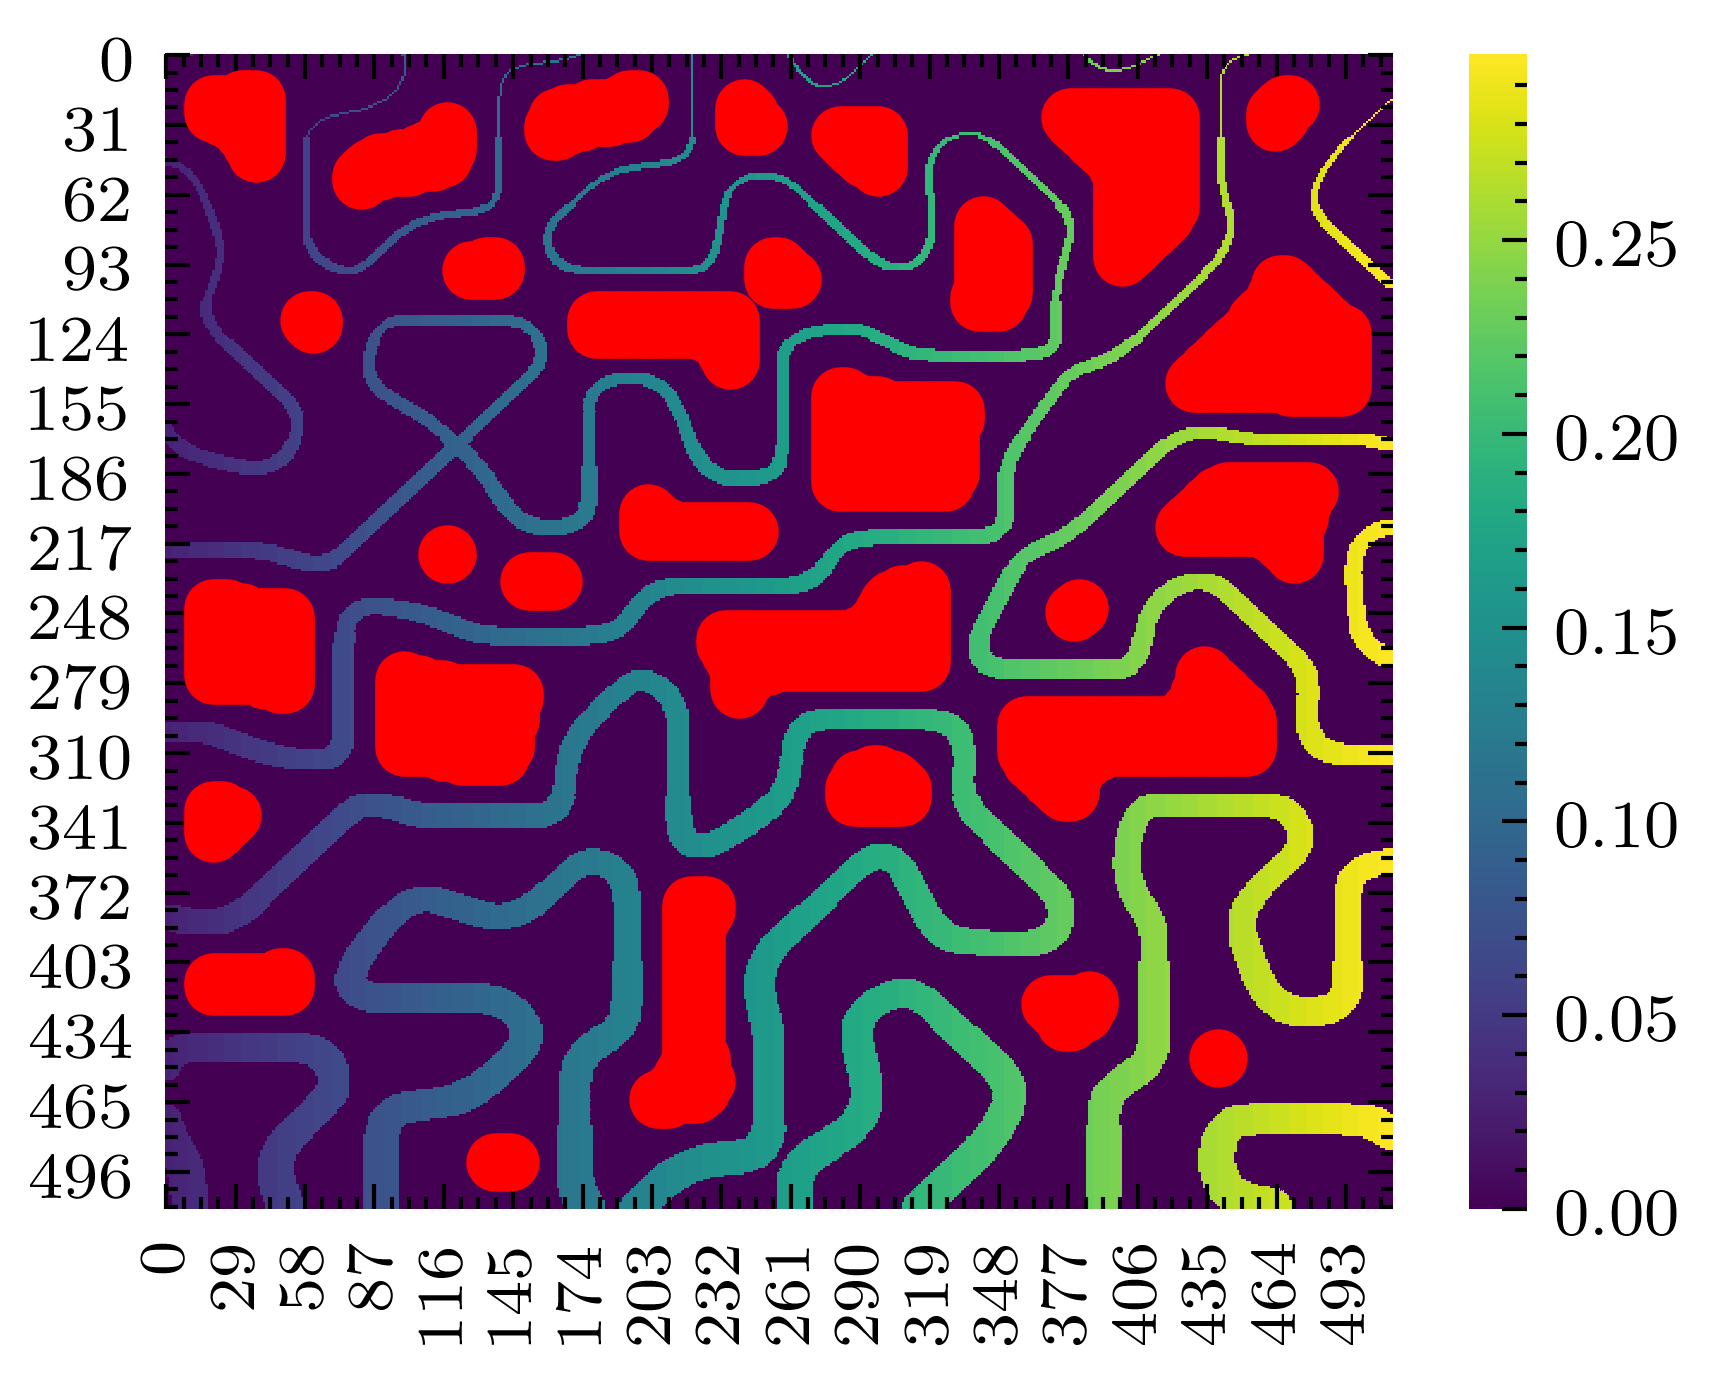
\includegraphics[width=\textwidth]{../img/3/spawn/flat-spawn-10.png}
        \caption{Flat regions}
    \end{subfigure}
    \begin{subfigure}[b]{0.5\textwidth}
        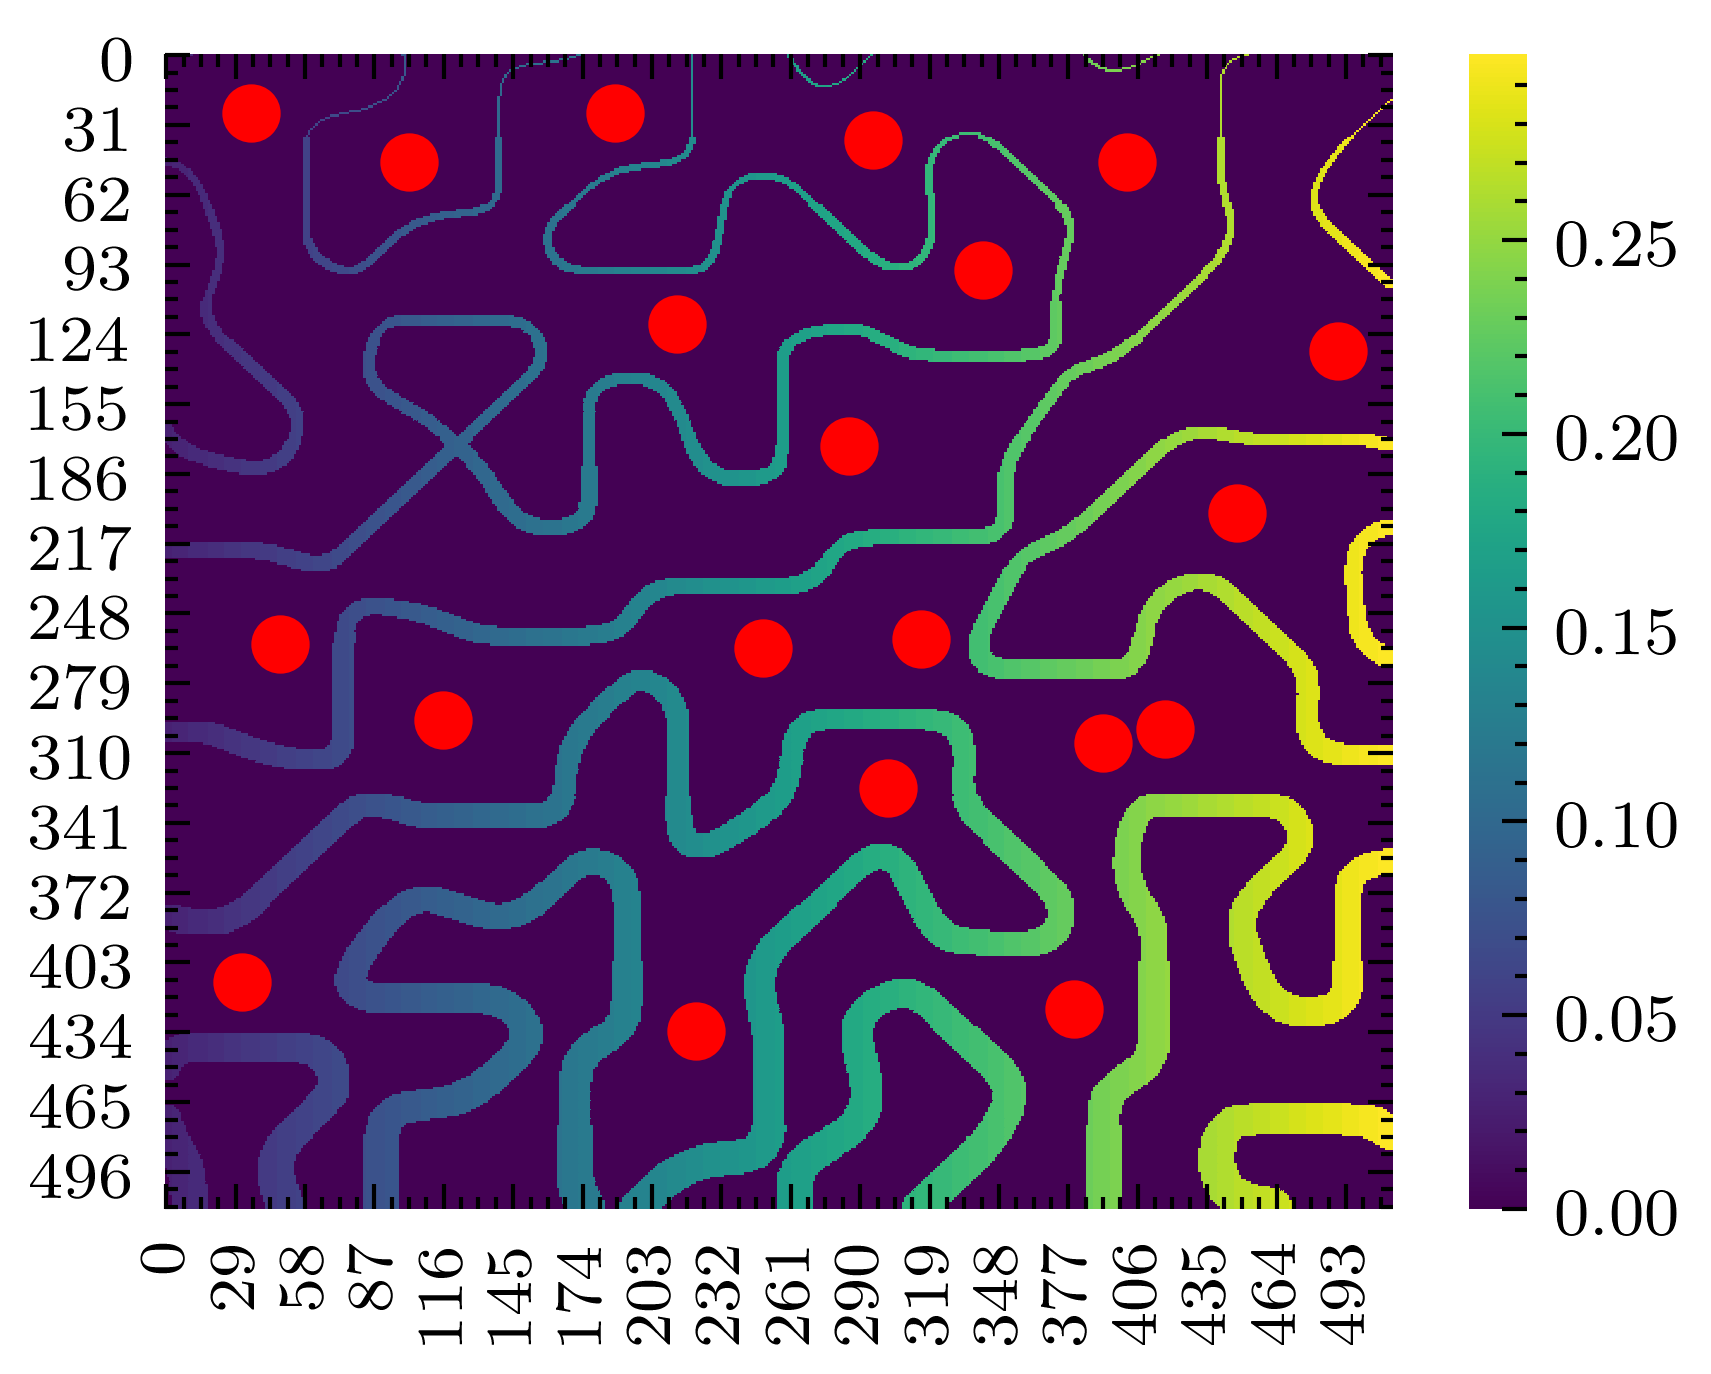
\includegraphics[width=\textwidth]{../img/3/spawn/spawn-10.png}
        \caption{K-Means with $k=20$}
    \end{subfigure}  
\label{fig: spawn-strat}
\caption{Selecting $20$ spawning points in \emph{bars1}}    
\end{figure}


\subsection{Postprocessing}
We now need to extract the patches for each pose $p_t$ of \emph{Krock} and compute the advancement for a given time window. To create the post-processing pipeline, we create an easy to use API \todo{link to the project} to define a cascade stream of function that is applied one after the other using a multi-thread queue to speed-up the process

First, we convert each \emph{.bag} file to a Pandas dataframe and cache them into \emph{.csv} files. We used an open source library that converts the bags file to dataframe to Python3 that we ported to Python3.\todo{library that convert the bags file}.
Then, we load the dataframes with the respective heightmaps and start the data cleaning process. We need to remove the rows in the first second of the simulation time to account for the robot spawning time. Then we eliminate all the entries where the \emph{Krock} pose was near the edges of a map, we used a threshold of $22$ pixels since we notice  \emph{Krock} getting stuck in the borders of the terrain during a simulation. 
After cleaning the data, we convert \emph{Krock} rotation express as a quaternion to Euler angle using the \emph{tf} package \todo{link to tf transform} from ROS. Then, we extract the $\sin$ and $\cos$ from the Euler orientation last component and store them in the dataframe.
Before caching again resulting dataframes into \emph{.csv} files, we convert the robot's position into heightmap's coordinates to use them later to crop the correct region of the map.

Finally, we load again the last stage and compute the advancement by projecting the pose's position, $x$ and $y$, in the current line. Then, we select a time window according to the store rate, for if we select two seconds we need to multiply the rate by two, so $50*2=100$ since \emph{Krock} published with a $50hz$ frequency. Once the time window is defined, we project $x$ and $y$ on the current line used the $\sin$ and $\cos$ values calculated before to get the advancement.

To create the patches, we first discover the maximum advancement for one second by running some simulations of \emph{Krock} on flat ground and averaging the advancement. For our robot, the maximum speed is $33cm/s$ Then, we multiply the maximum displacement by the number of seconds we are interested in. We can now crop the corresponding region in the heightmap by including the whole \emph{Krock}'s footprint and the maximum advancement. The following figure visualizes the patch extraction process. 
\todo[inline]{figure that shows Krock somewhere with the patch bouding boxed}. Lastly, we create a dataframe containing the map coordinates, the advancement, and the patches paths for each simulation run and savewe store them to disk as \emph{.csv} files. 

The whole pipeline takes less than one hour to run the first time with 16 threads, and, once it is cached, less than fifteen minutes to extract the patches. 

Once we extract the patches, we can always compute again the advancement without re-running the whole pipeline. The next figure show proposed pipeline.
\begin{figure}[H] 
\centering
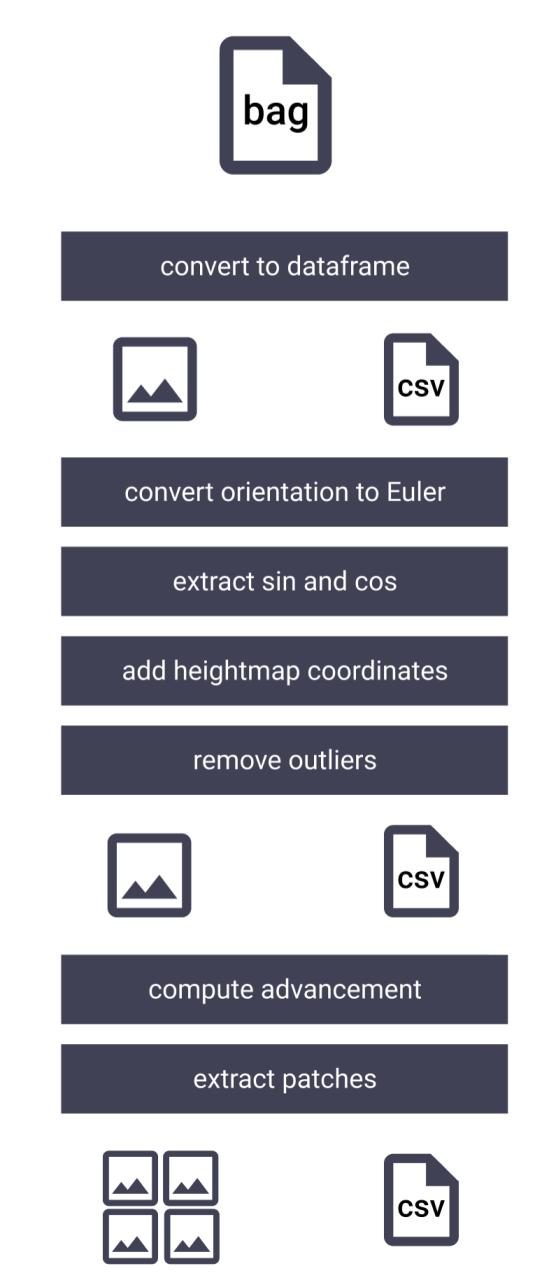
\includegraphics[width=0.4\textwidth]{../img/postprocessing-pipeline.jpg}
\caption{Postprocessing}
\label{fig: postprocessing-pipeline}
\end{figure}
\subsection{Estimator}

\subsubsection{Vanilla Model}
\subsubsection{ResNet}

We decide to use a Residual Network, ResNet \cite{he2015deep}, variant. Residual network are deep convolutional
networks consisting of many stacked \" Residual Units \". Intuitively, the residual unit allows the input of a layer to contribuite to the next layer's input by beeing added to the current layer's output. Due to possible different features dimension, the input must go thought and identify map to make the addition possible. This allows a stronger gradient flows and mitigates the degradation problem. A \"Residual Units \" is composed by a two $3x3$ \emph{Convolution}, \emph{Batchnorm} \cite{ioffe2015batch} and a \emph{Relu} blocks. Formally, it is defined as: 
\begin{equation}
	\mathbf{y}=\mathcal{F}\left(\mathbf{x},\left\{W_{i}\right\}\right)+h(\mathbf{x})
	\label{eq : resnet}
\end{equation}
Where, $x$ and $y$ are the input and output vector of the layers considered. The function $\mathcal{F}\left(\mathbf{x},\left\{W_{i}\right\}\right)$ is the residual mapping to be learn and $h$ is the identity mapping. The next figure visualises the equation.

\begin{figure}[H]
	\centering
	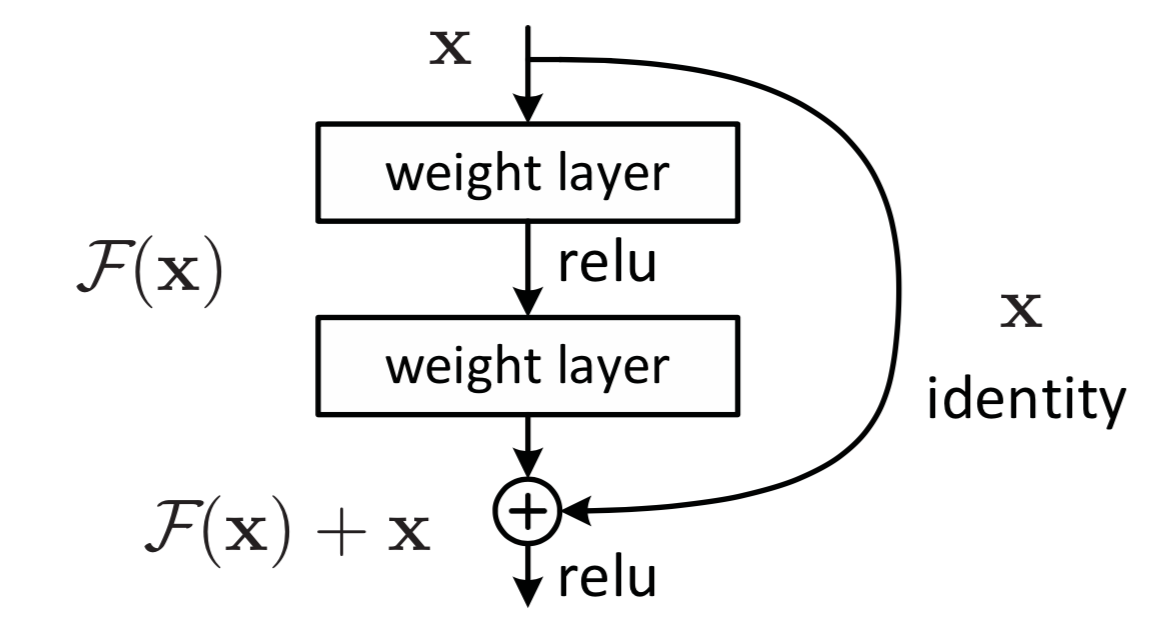
\includegraphics[scale=0.3]{../img/implementation/estimator/resnet_block.png}
	\caption{\emph{Resnet} block.}
\end{figure}
When the input and output shapes mistmatch, the \emph{identity map} is applyed to the input as a $3x3$ Convolution with a stride of 2 to mimic the polling operator. A single block is composed by a $3x3$ \emph{Convolution}, \emph{Batchnorm} and a \emph{Relu} activation function. 

Following the recent work of He et al. \cite{he2015identity} we adopt \emph{pre-activation} in each block.\emph{Pre-activation} works by just reverse the order of the operations in a block.

\begin{figure}[H]
	\centering
	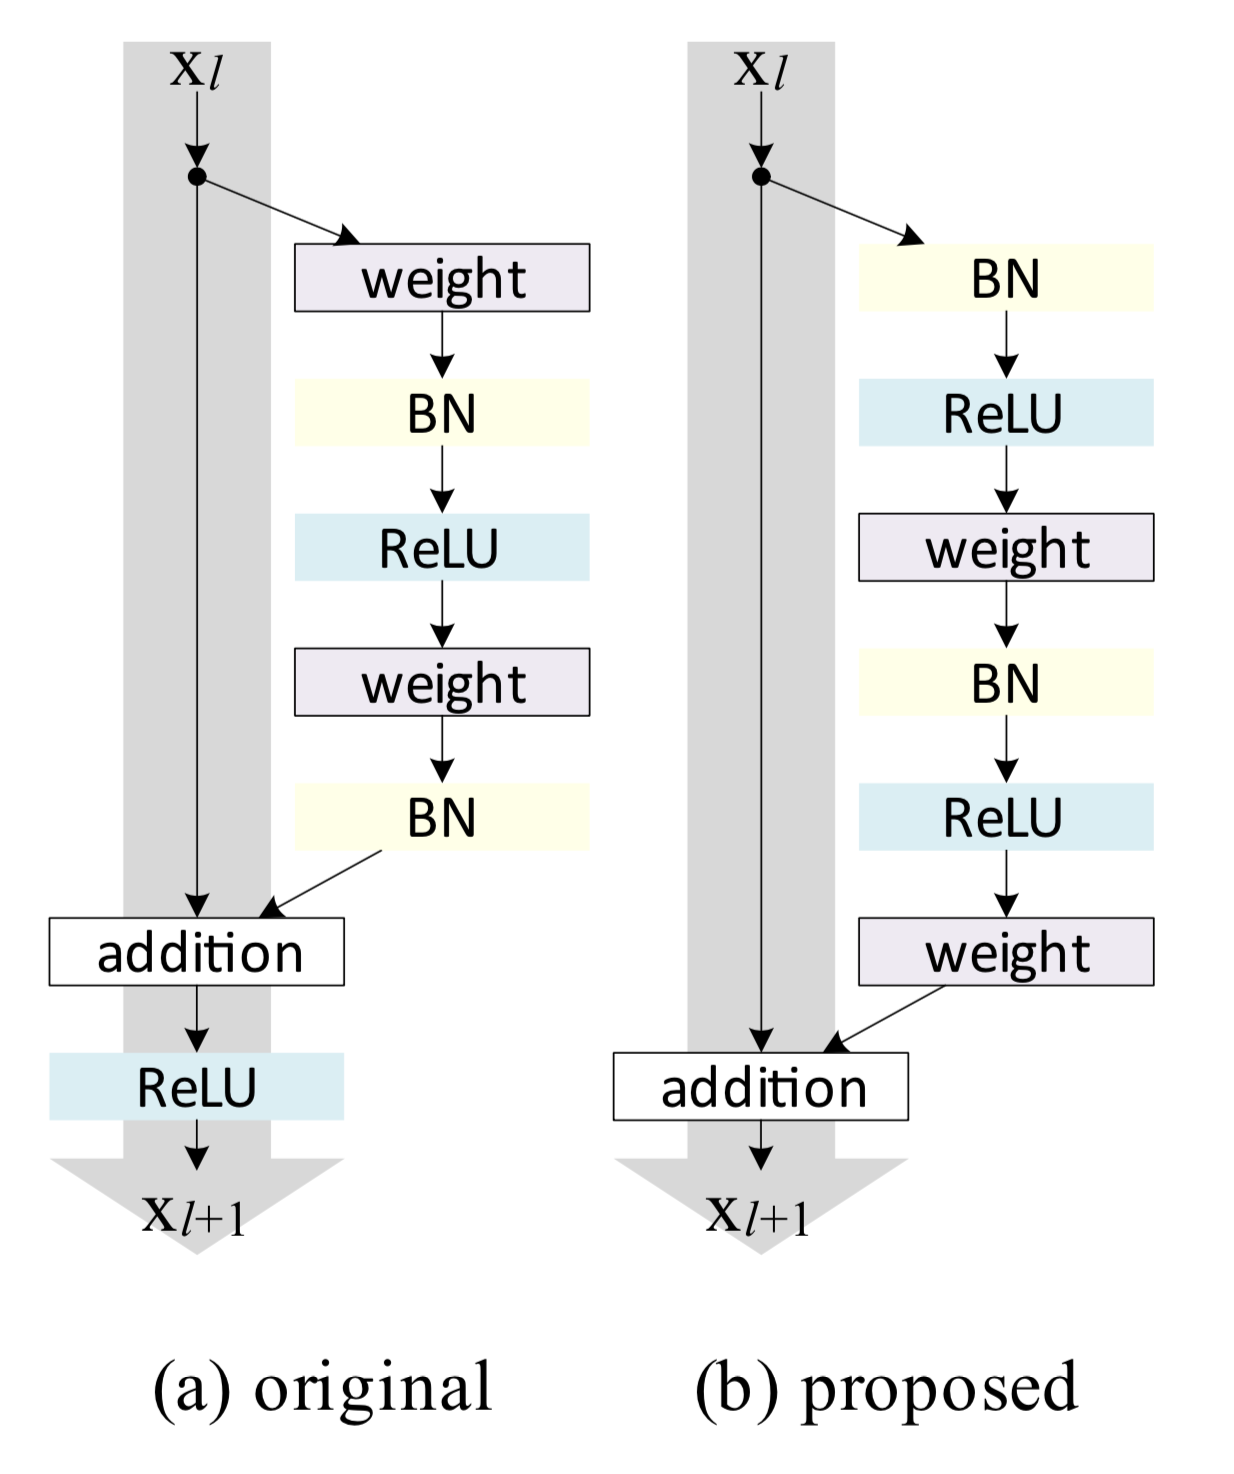
\includegraphics[scale=0.2]{../img/implementation/estimator/preactivation.png}
	\caption{\emph{Preactivation}}
\end{figure}
Finally, we also used the \emph{Squeeze and Excitation} (SE) module \cite{hu2017squeeze}. It is a form of attention that weights the channel of each convolutional operation by learnable scaling factors. The next figure visualises the SE module.
\begin{figure}[H]
	\centering
	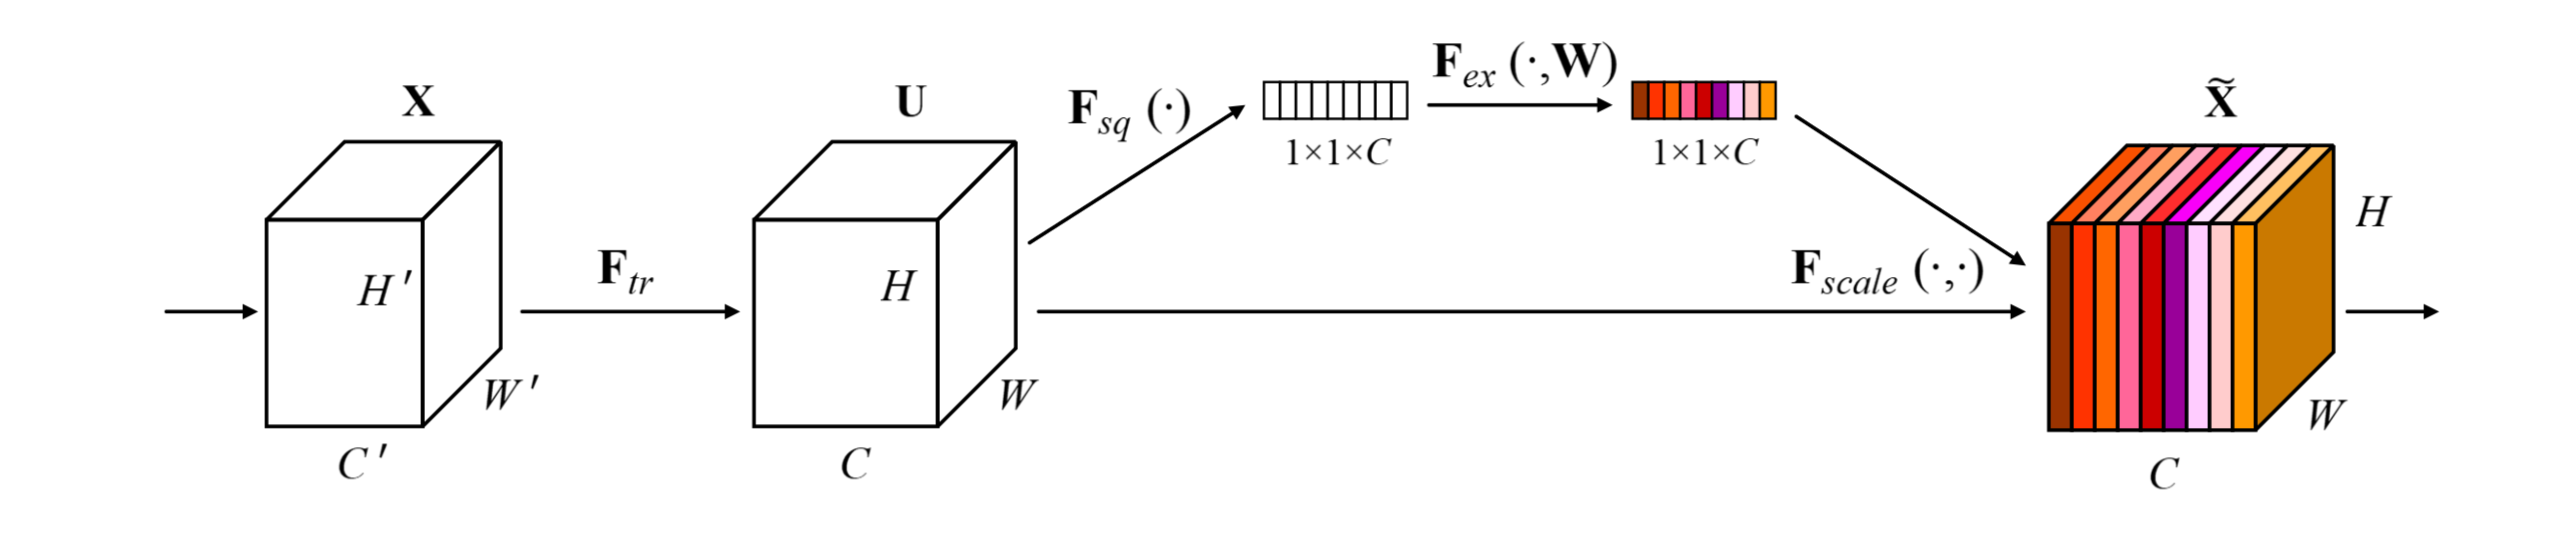
\includegraphics[width=\linewidth]{../img/implementation/estimator/se.png}
	\caption{\emph{Preactivation}}
\end{figure}
Our network differs is composed by $n$ ResNet blocks, a depth of $d$ and a channel incrementing factor of $2$. We select $n=1$ and $d=3$ with a starting channel size of $16$, we called this model architecture \emph{micro-resnet}. 

\begin{table}[H]
    \centering
    \begin{tabular}{|lc|}
        \hline
        & micro resnet \\
        \hline 
        & depth $=3$ \\ 
        \hline 
        & n $=1$ \\
        \hline
     &$3 \ x\ 3,\ 16 \ stride\ 1$ \\ 
     \hline
     &$2 \ x\ 2$ max-pool \\ 
     \hline
     & \\
     &$\begin{bmatrix}
      3\ x\ 3, & 16 \\
      3\ x \ 3, & 16 \\  
     \end{bmatrix}$ x 1 \\ 
     & \\
     \hline     
     & SE-module\\ 
     \hline     
     & \\
     &$\begin{bmatrix}
        3\ x \ 3, & 32 \\
        3\ x\ 3, & 32 \\  
       \end{bmatrix}$ x 1 \\\
       & \\ 
       \hline
       & SE-module\\ 
       \hline
       & \\
       &$\begin{bmatrix}
        3\ x \ 3, & 64 \\
        3 \ x \ 3, & 64 \\  
       \end{bmatrix}$ x 1 \\  
       & \\
       \hline     
       & SE-module\\ 
       \hline
       & average pool, $1$-d fc, softmax \\ 
       \hline

    \end{tabular}
    \caption{\emph{micro-resnet} architecture}
\end{table}

\todo[inline]{add model picture}
\subsubsection{Normalization}
Before feeding the data to the models, we need make the patches height invariant. This must be done to correctly normalize different patches taken from different maps with different height scaling factor. We subtract the krock's position height from the patch to correctly center the height.. The following figure shows the normalization process on the patch with the square in the middle.
\begin{figure}[H]
    \begin{subfigure}[b]{0.5\textwidth}
        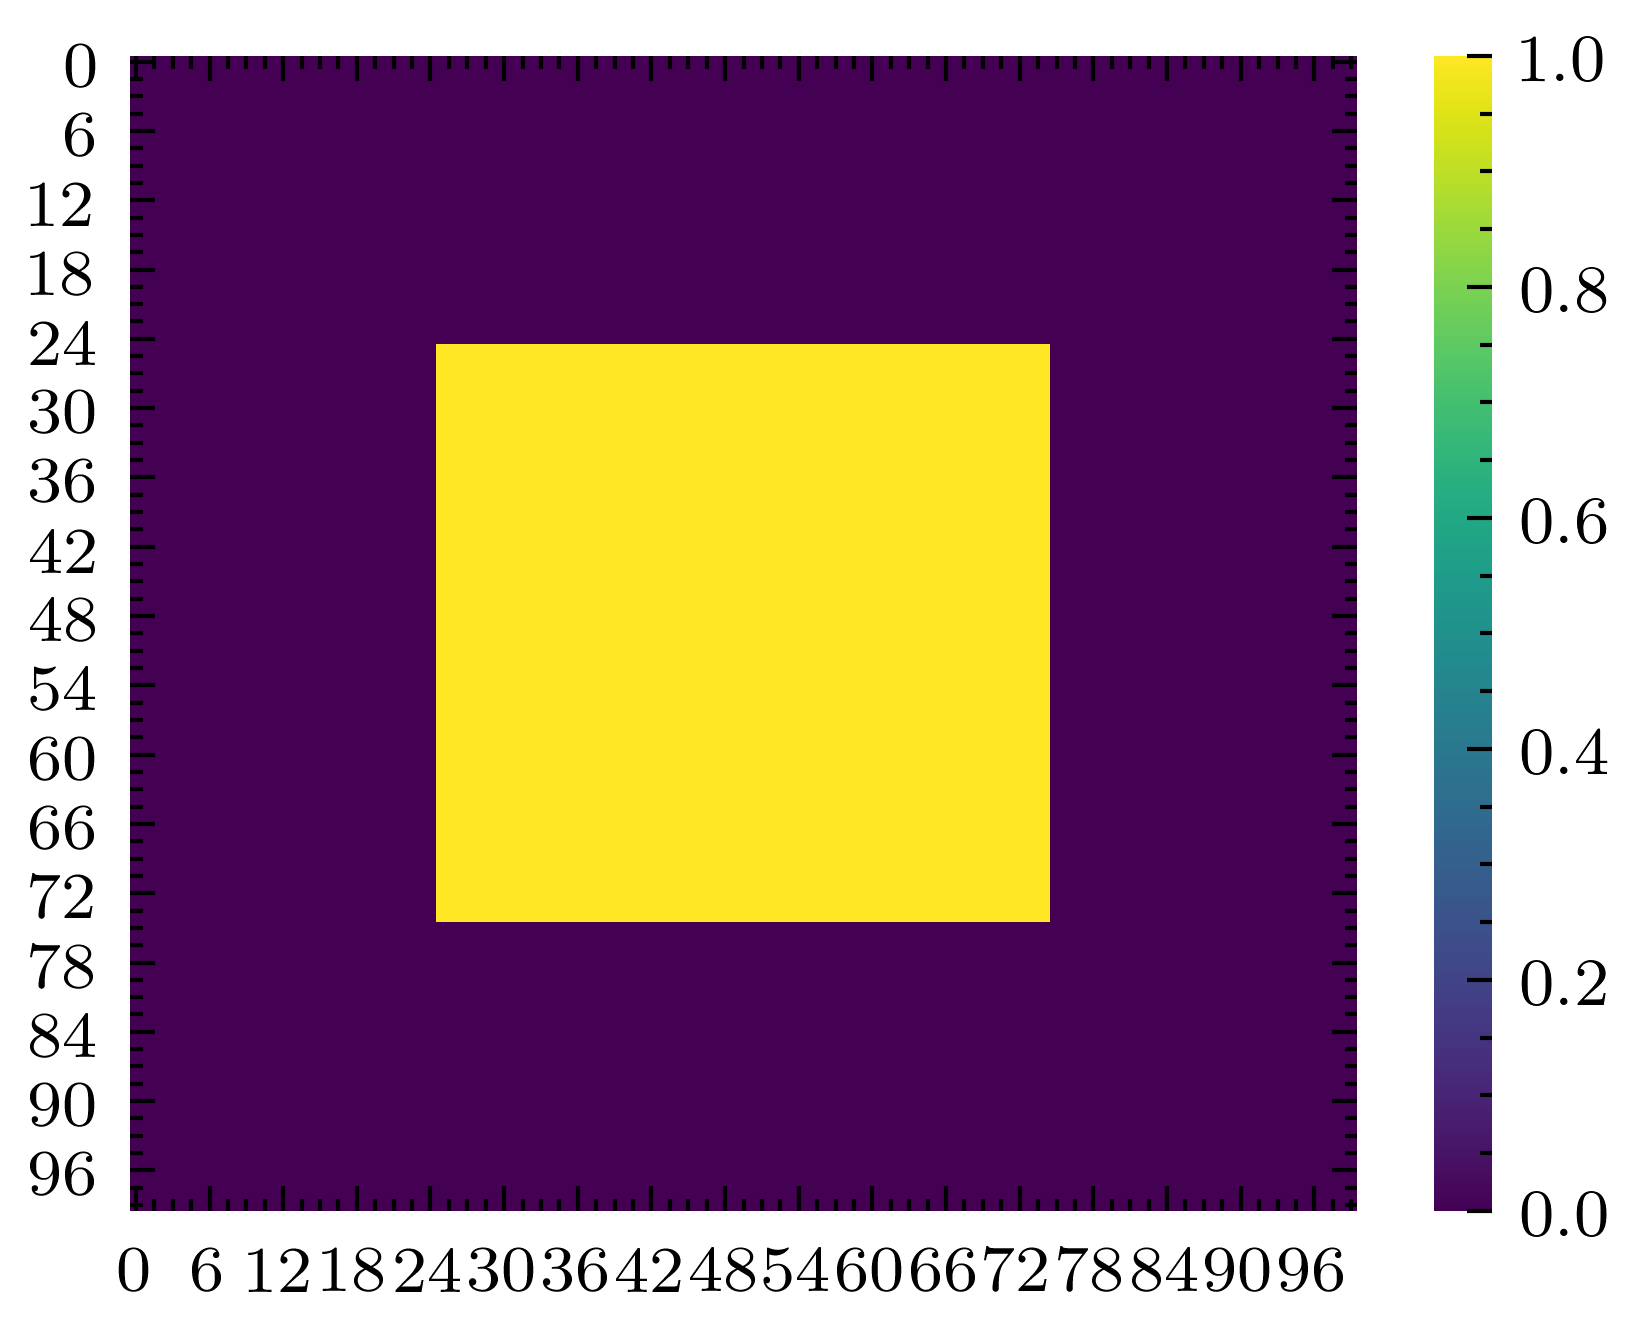
\includegraphics[width=\textwidth]{../img/data-aug/2d/square-middle.png}
        \caption{Input}
    \end{subfigure}
    \begin{subfigure}[b]{0.5\textwidth}
        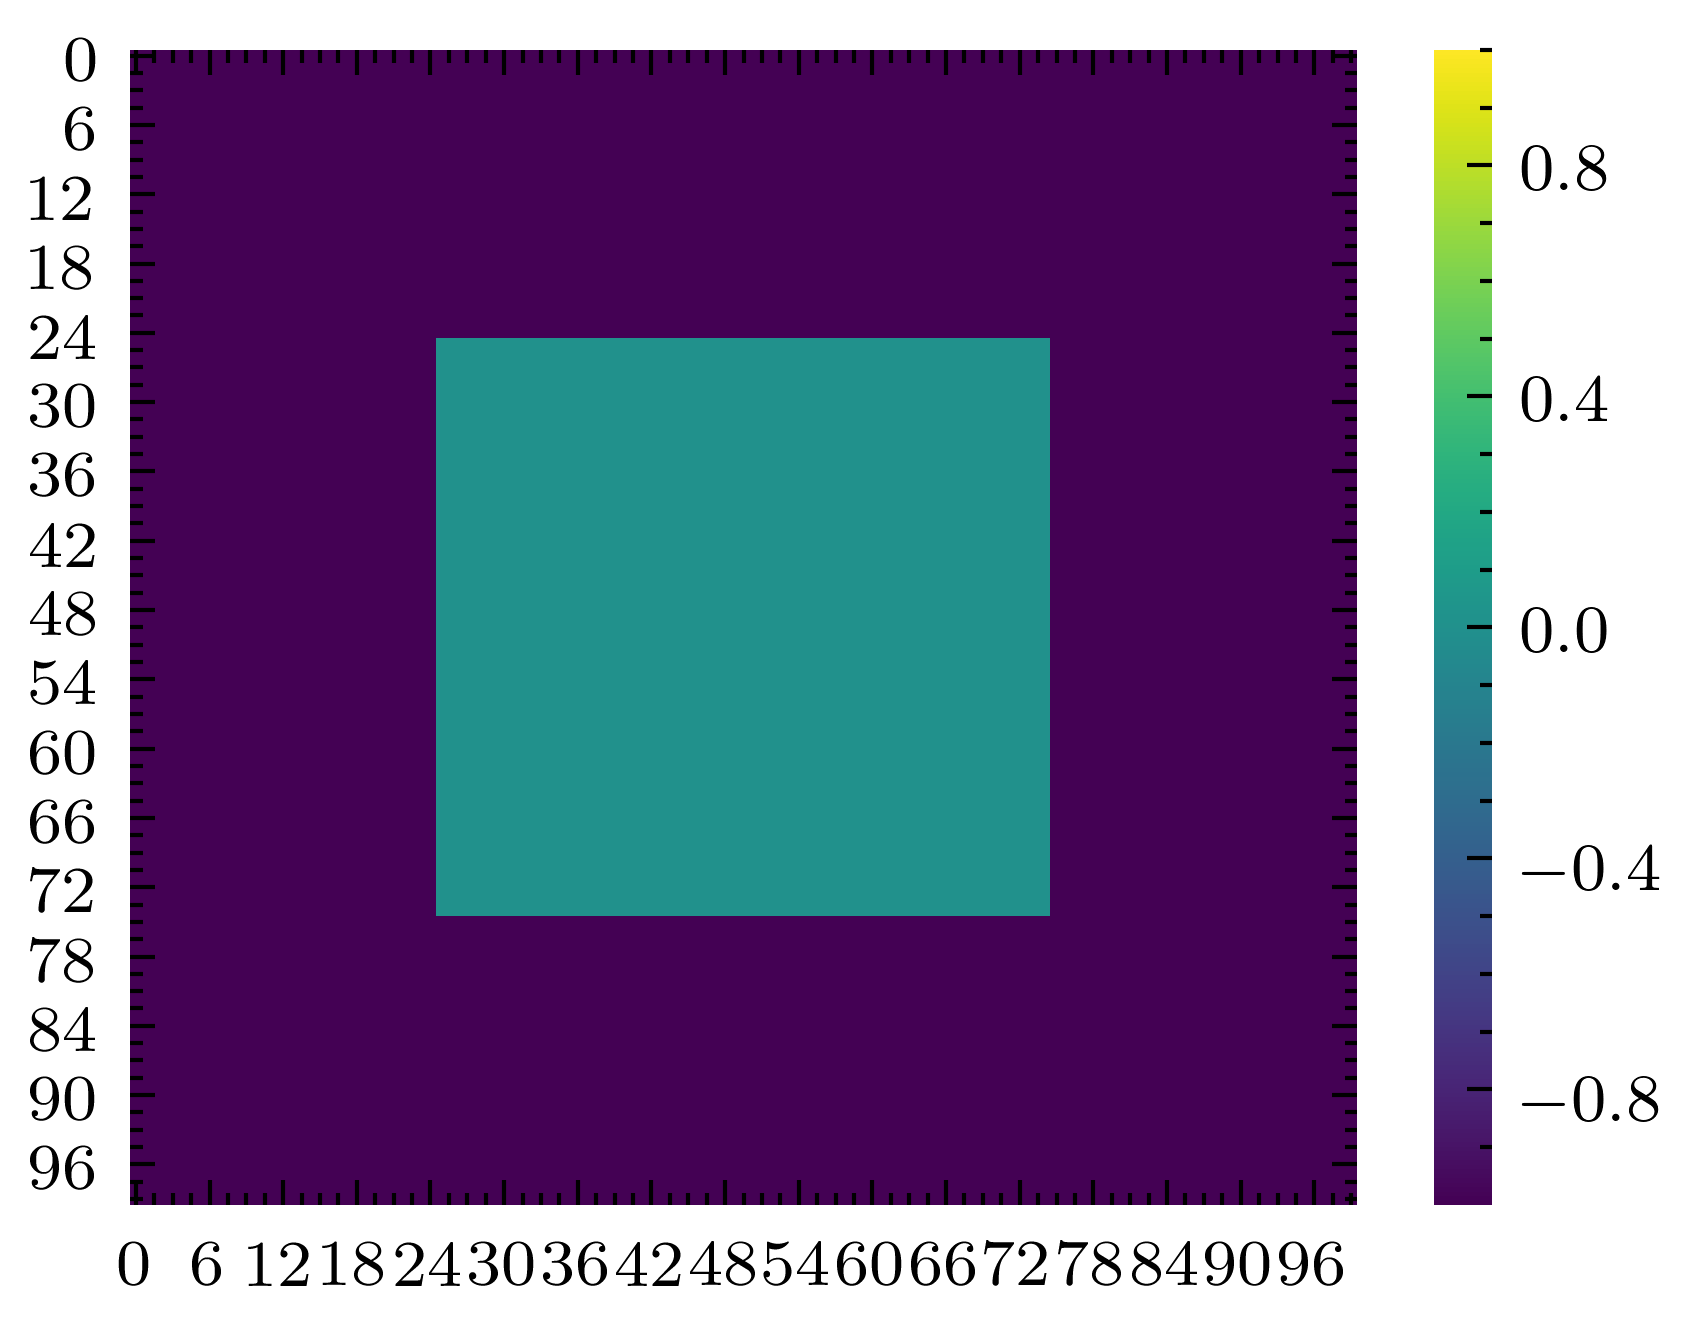
\includegraphics[width=\textwidth]{../img/data-aug/2d/square-middle-center.png}
        \caption{Height centered}
    \end{subfigure}  
    
          \begin{subfigure}[b]{0.5\textwidth}
        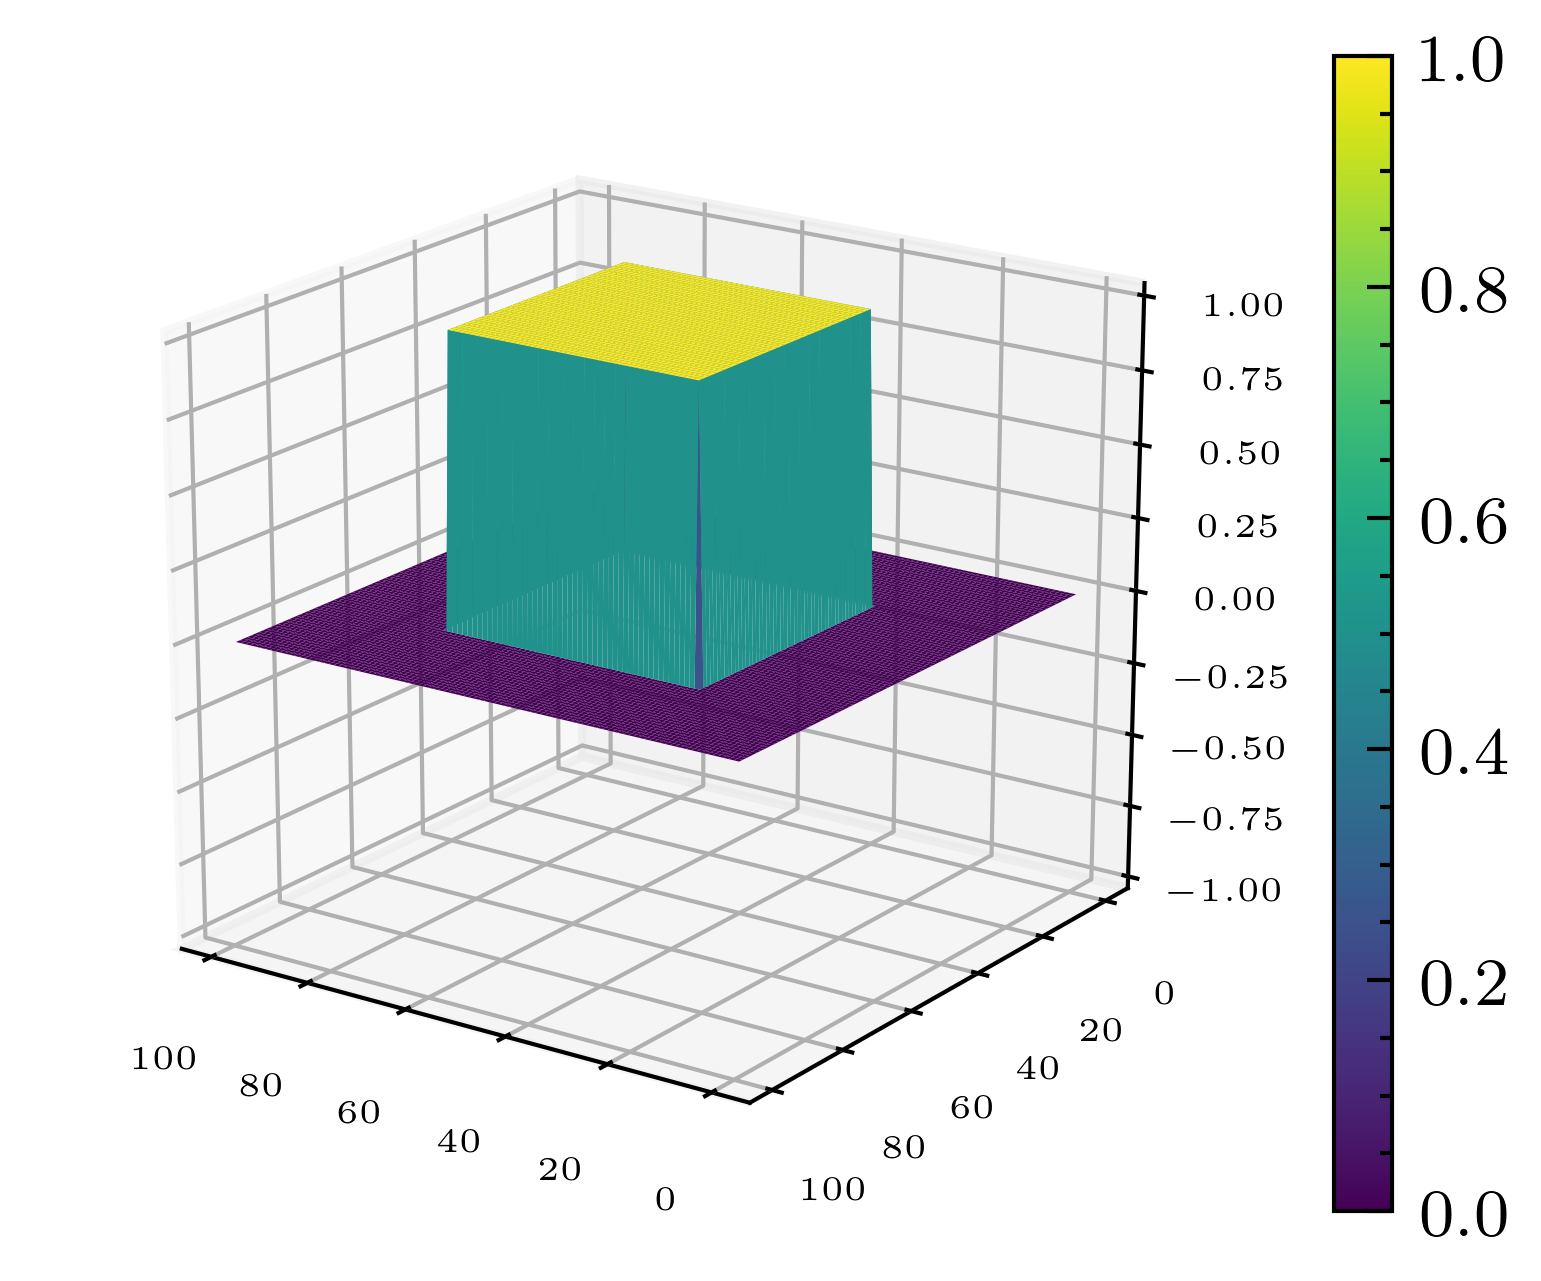
\includegraphics[width=\textwidth]{../img/data-aug/3d/square-middle.png}
        \caption{Input}
    \end{subfigure}
    \begin{subfigure}[b]{0.5\textwidth}
        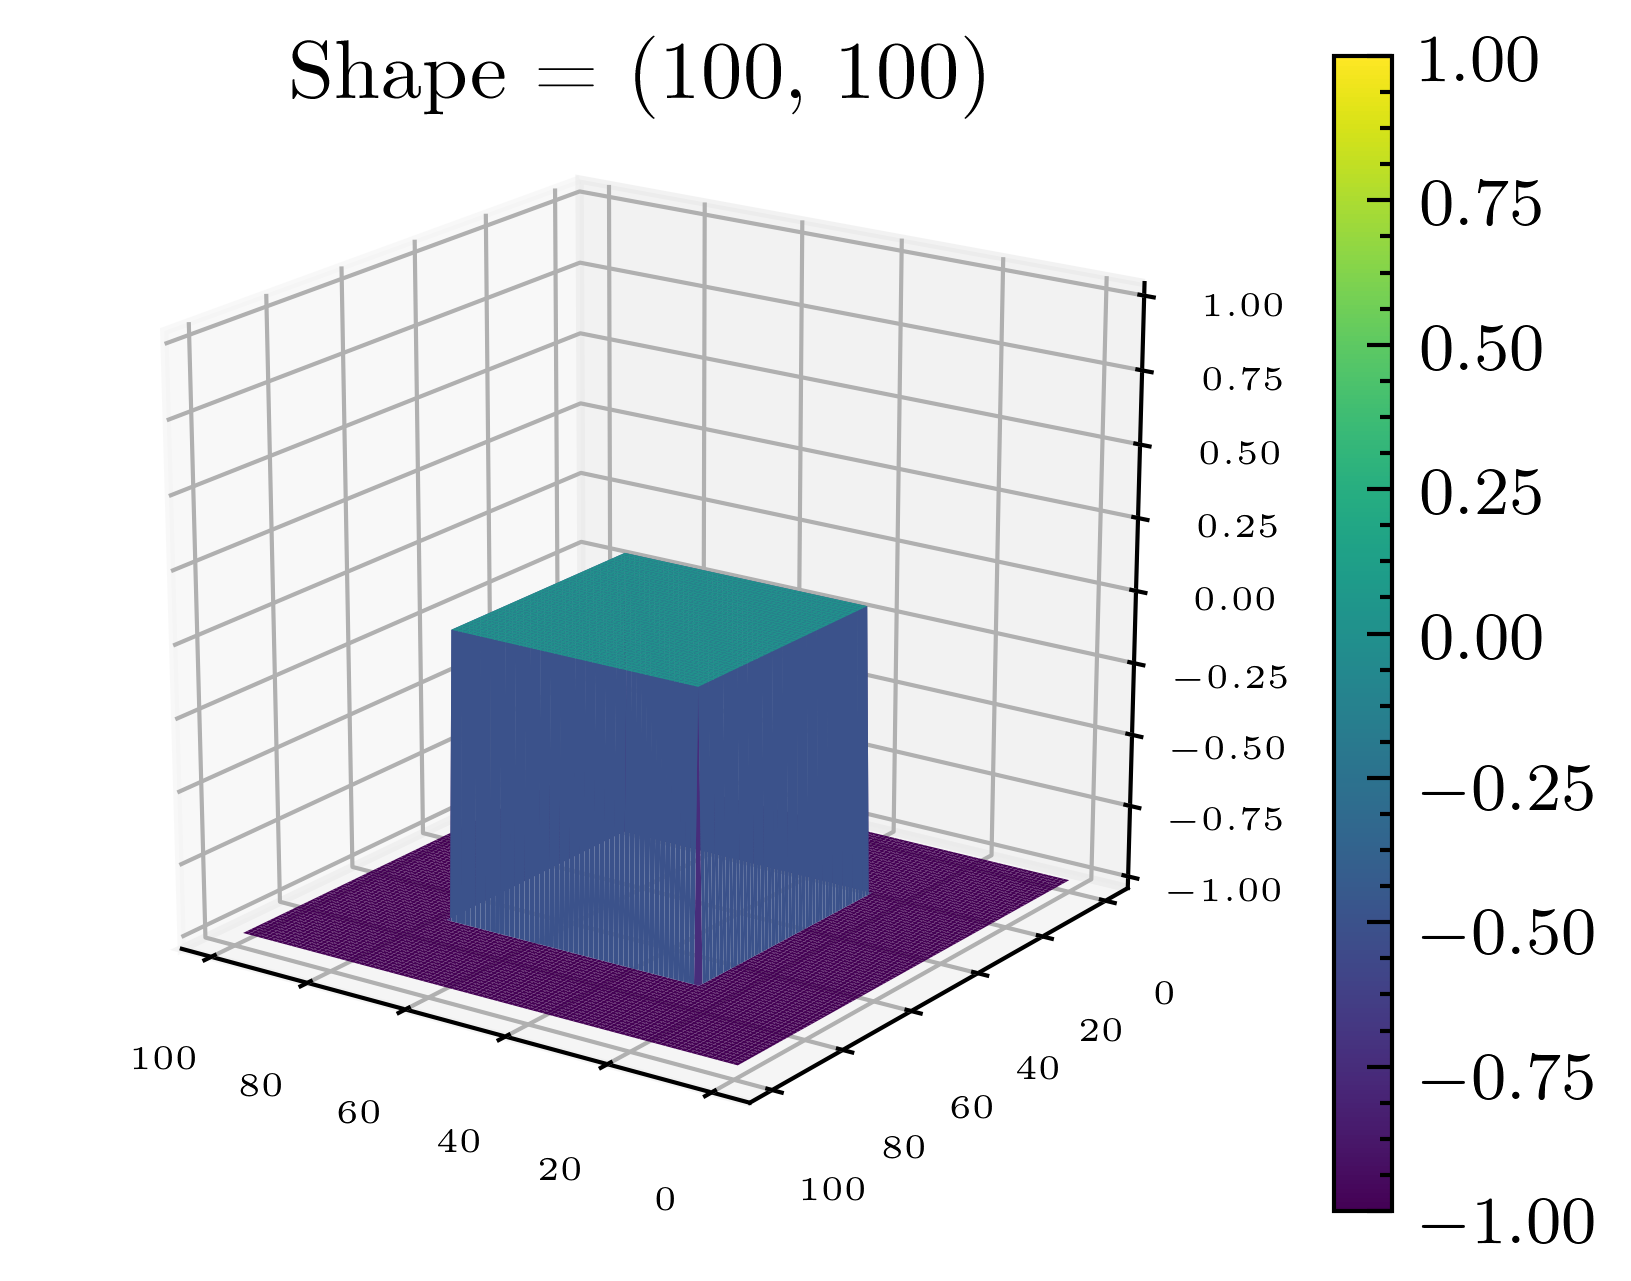
\includegraphics[width=\textwidth]{../img/data-aug/3d/square-middle-center.png}
        \caption{Height centered}
    \end{subfigure}  
\label{fig: center}
\caption{Normalization process}    
\end{figure}

\subsubsection{Data Augmentation}
Data augmentation is used to change the input of a model using different techniques to change it in order to produce more training examples. Since our inputs are heightmaps we cannot utilise the classic image manipulations such as shifts, flips and zooms. Imagine that we have a patch with a wall in front of it, if we random rotate the image the wall may go in a position where the patch it is now traversable but its label is still not traversable, we have to be more creative. We decided to apply dropout, coarse dropout and random simplex noise since they are traversability invariant. To illustrate those techniques we are going to use the following example patch of size $100x100$.
\begin{figure}[H]
    \begin{subfigure}[b]{0.5\textwidth}
        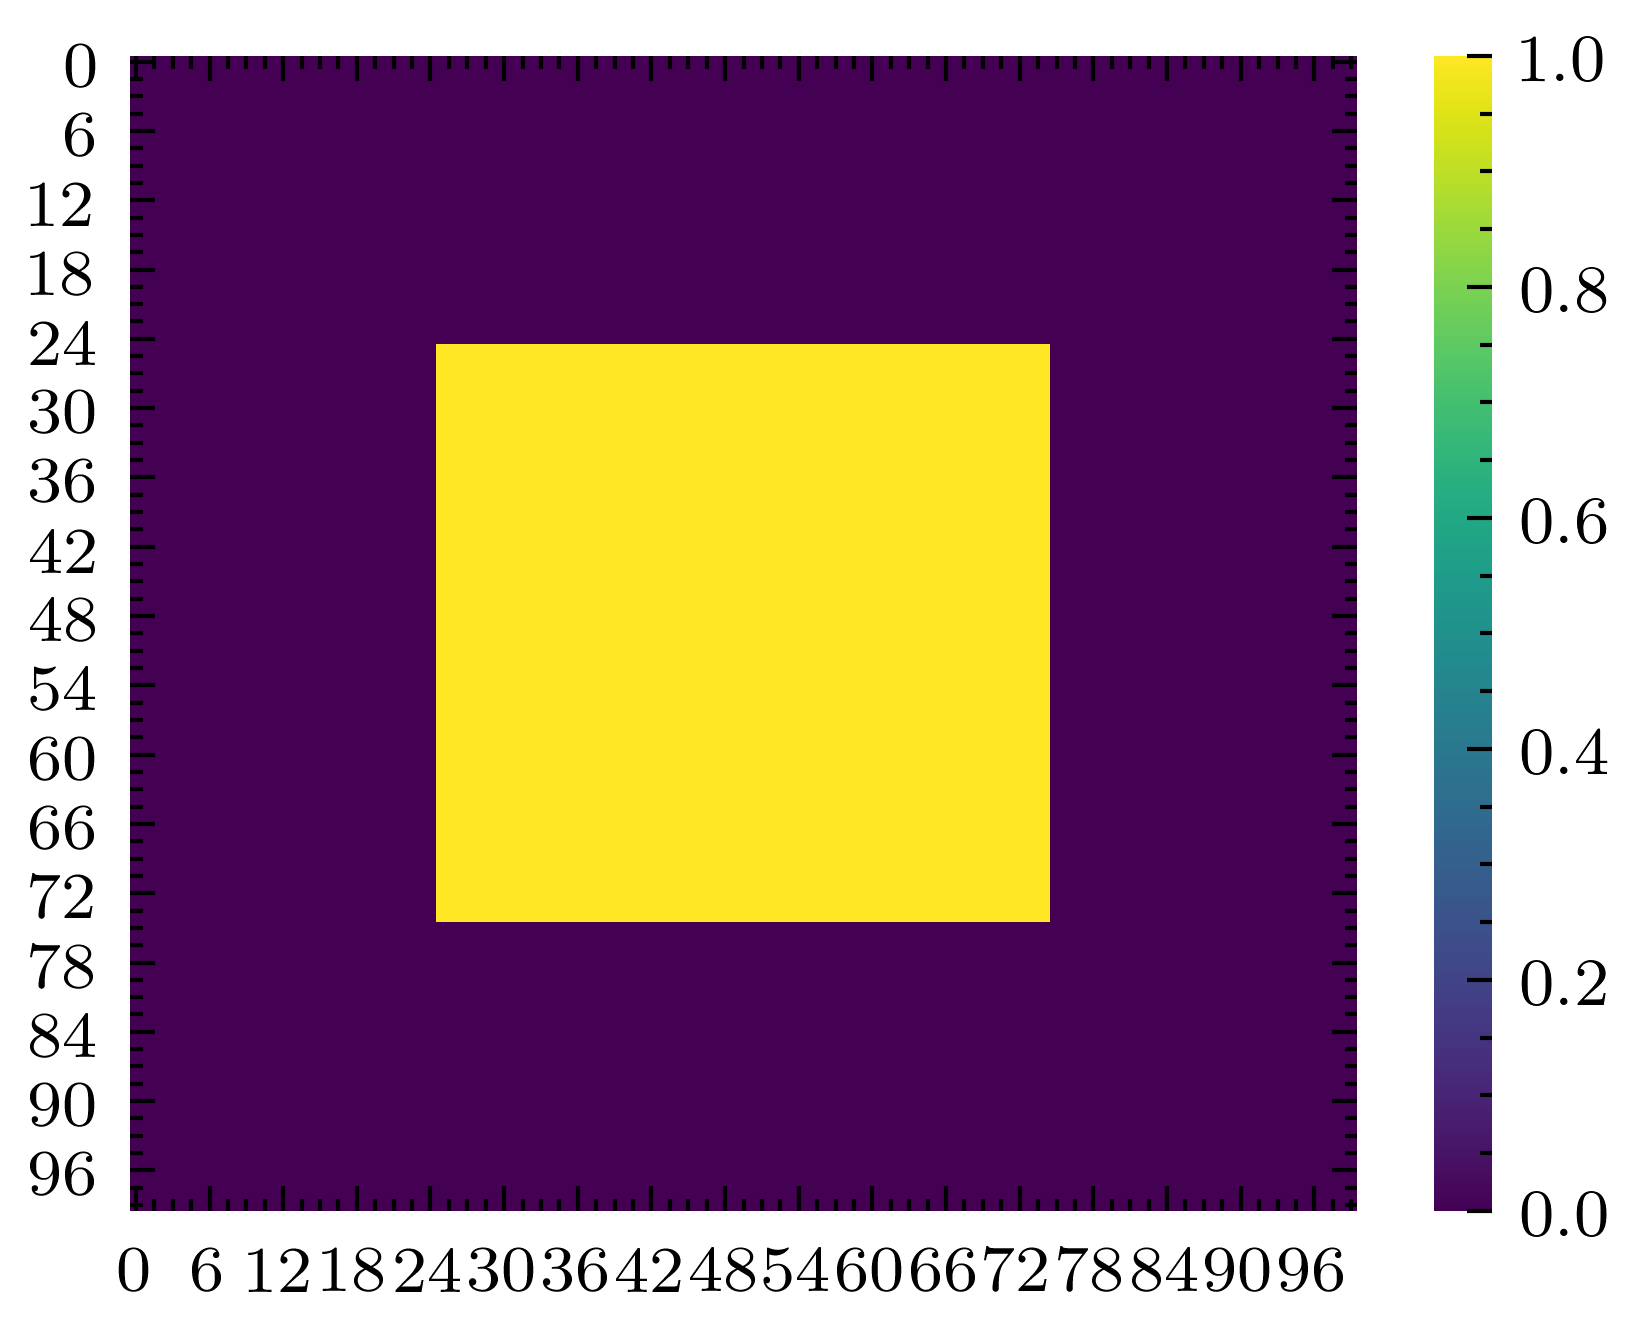
\includegraphics[width=\textwidth]{../img/data-aug/2d/square-middle.png}
    \end{subfigure}
    \begin{subfigure}[b]{0.5\textwidth}
        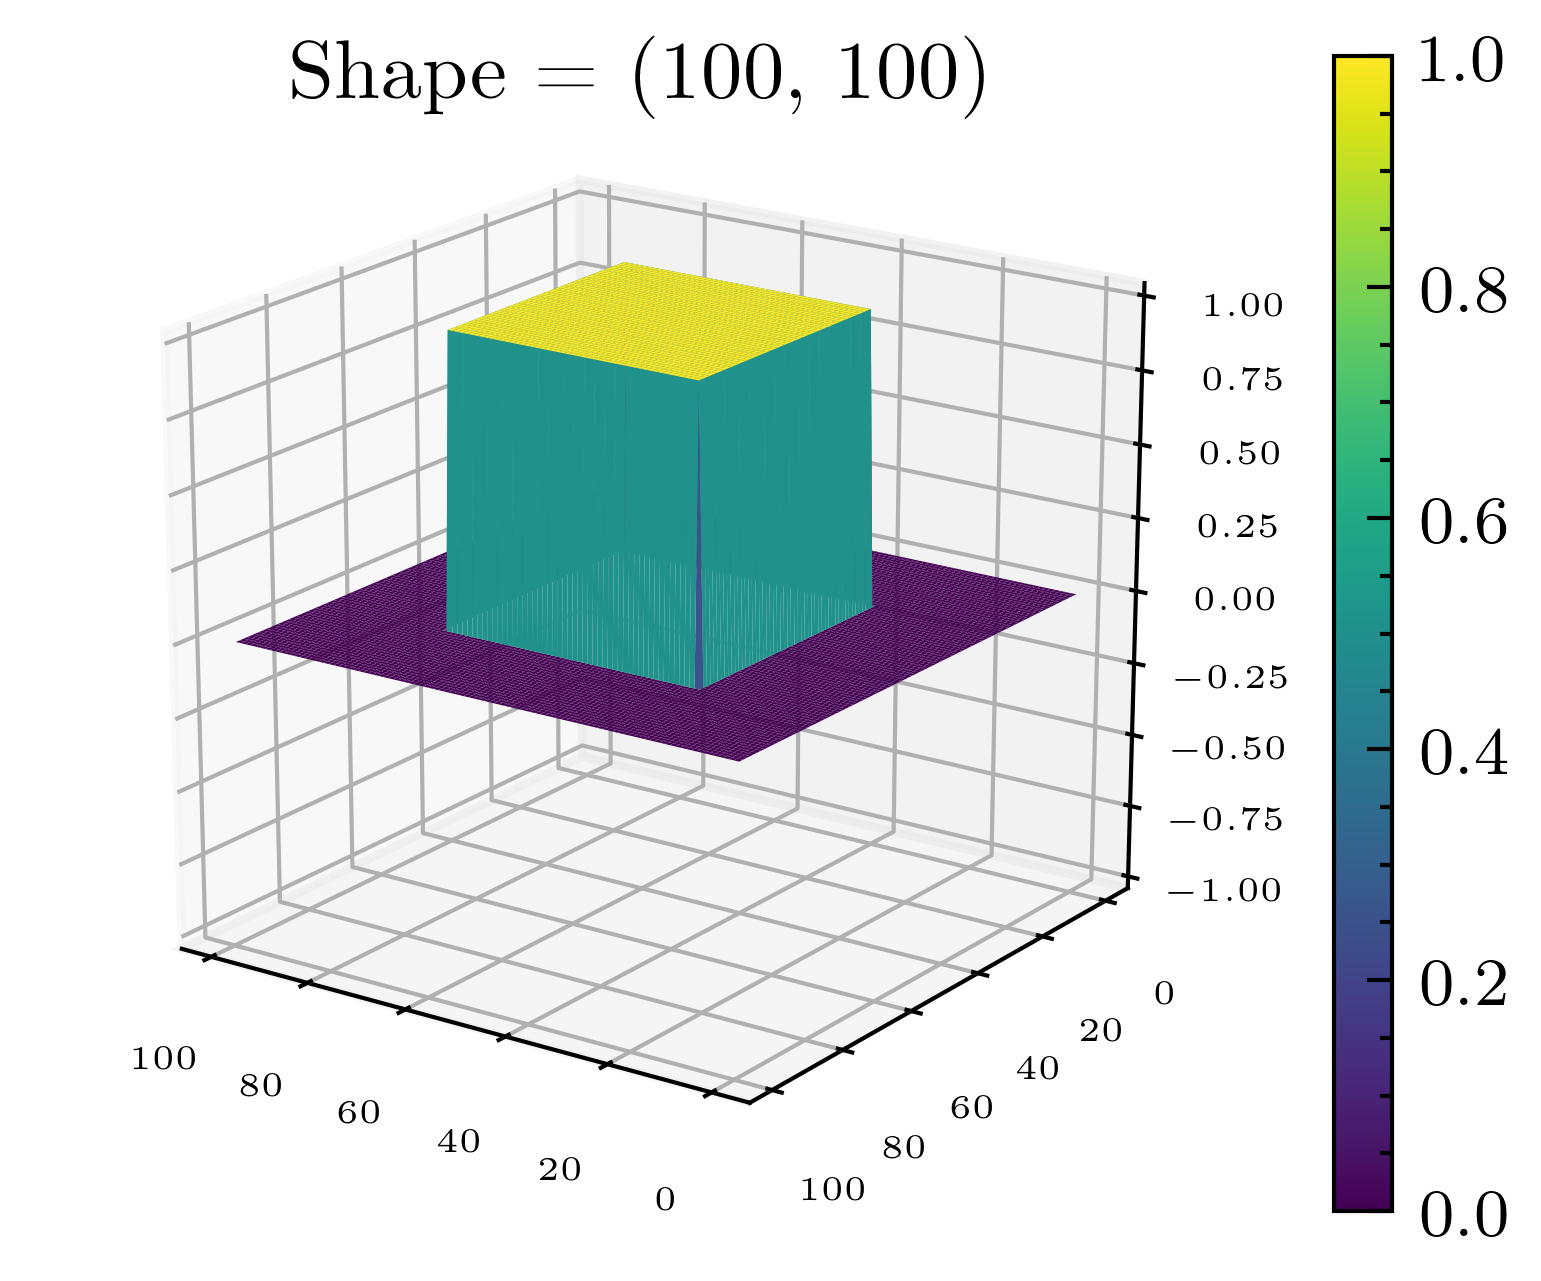
\includegraphics[width=\textwidth]{../img/data-aug/square-middle.png}
    \end{subfigure}    
\label{fig: square-patch}
\caption{A patch with a square in the middle}    
\end{figure}
\paragraph{Dropout} is a technique to randomly set some pixels to zero, in our case we flat some random pixel in the patch. 
\paragraph{Coarse Dropout} similar to dropout, it sets to zero random regions of pixels.
\paragraph{Simplex Noise} is a form of Perlin noise that is mostly used in ground generation. Our idea is to add some noise to make the network generalise better since lots of training maps have only obstacles in flat ground. Since it is computational expensive, we randomly fist apply the noise to five hundred images with only zeros. Then, we randomly scaled them and add to the input image.
\begin{figure}[H]
    \centering

        \begin{subfigure}[b]{0.45\textwidth}
            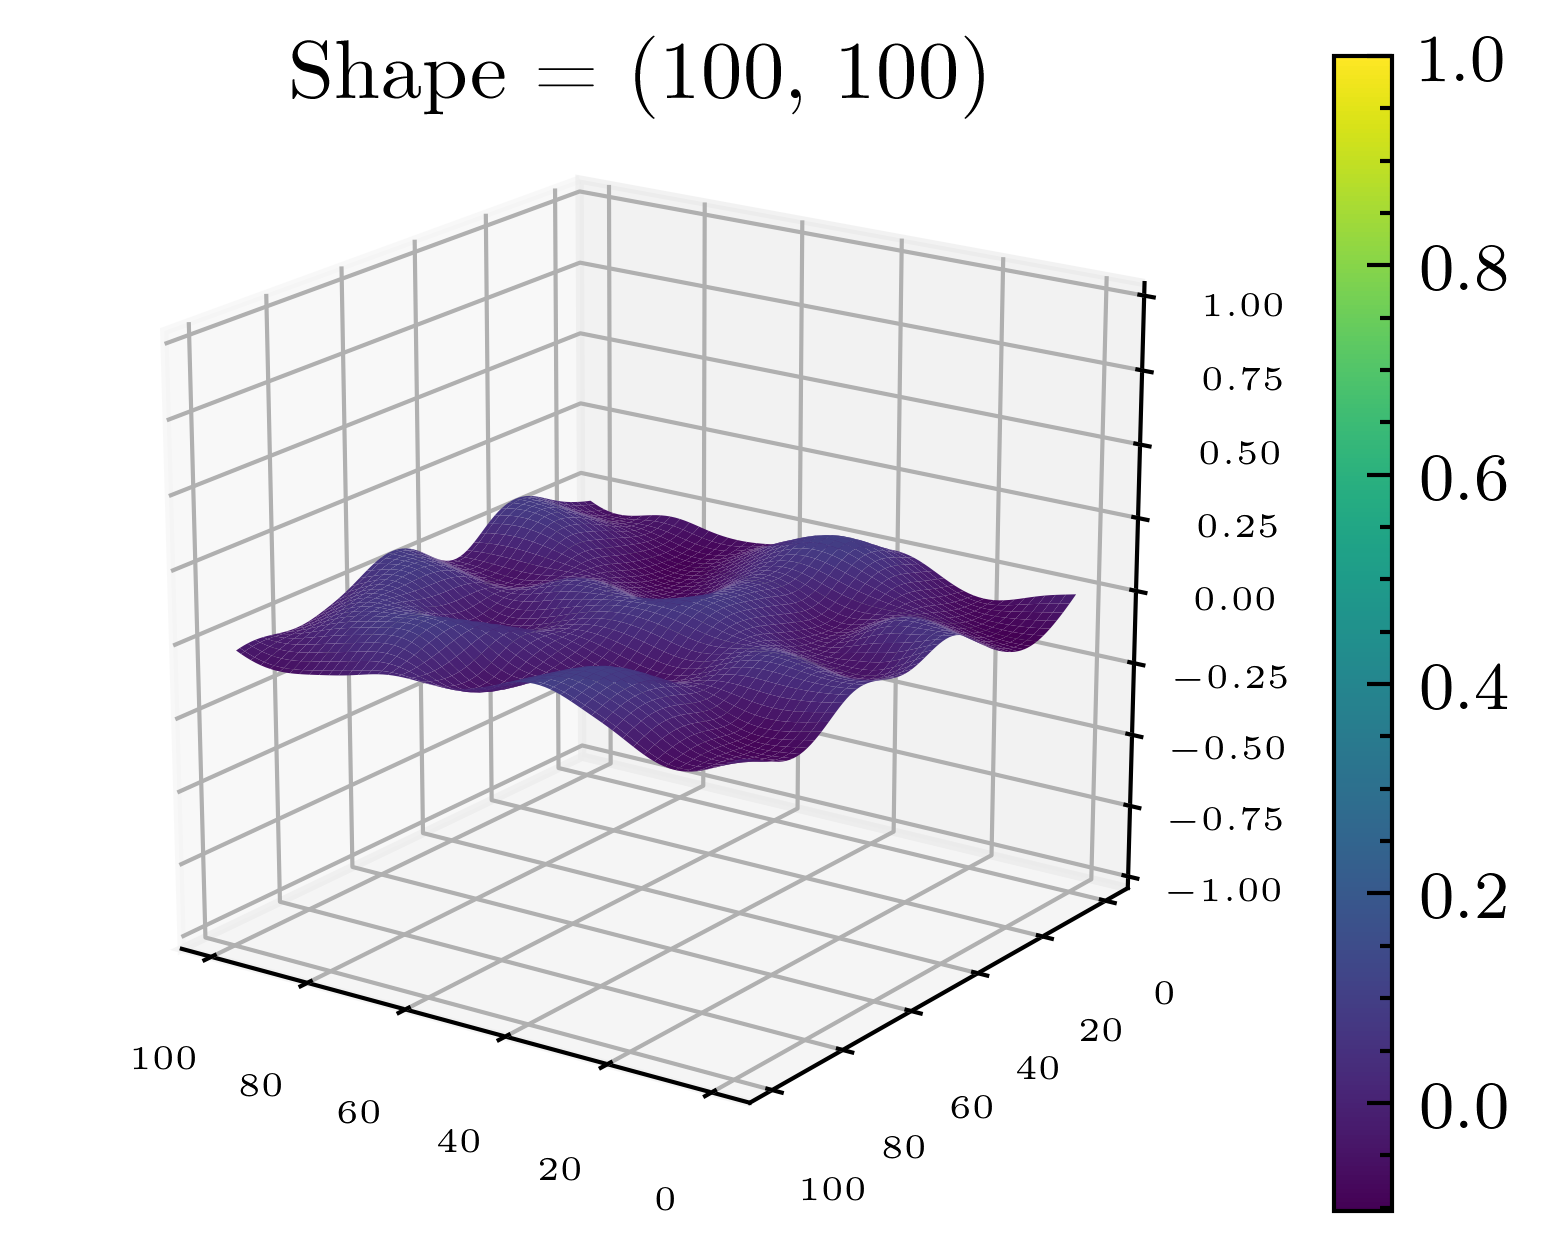
\includegraphics[width=\textwidth]{../img/data-aug/3d/simplex1.png}
            \caption{Features size = 10}
        \end{subfigure}
        \begin{subfigure}[b]{0.45\linewidth}
            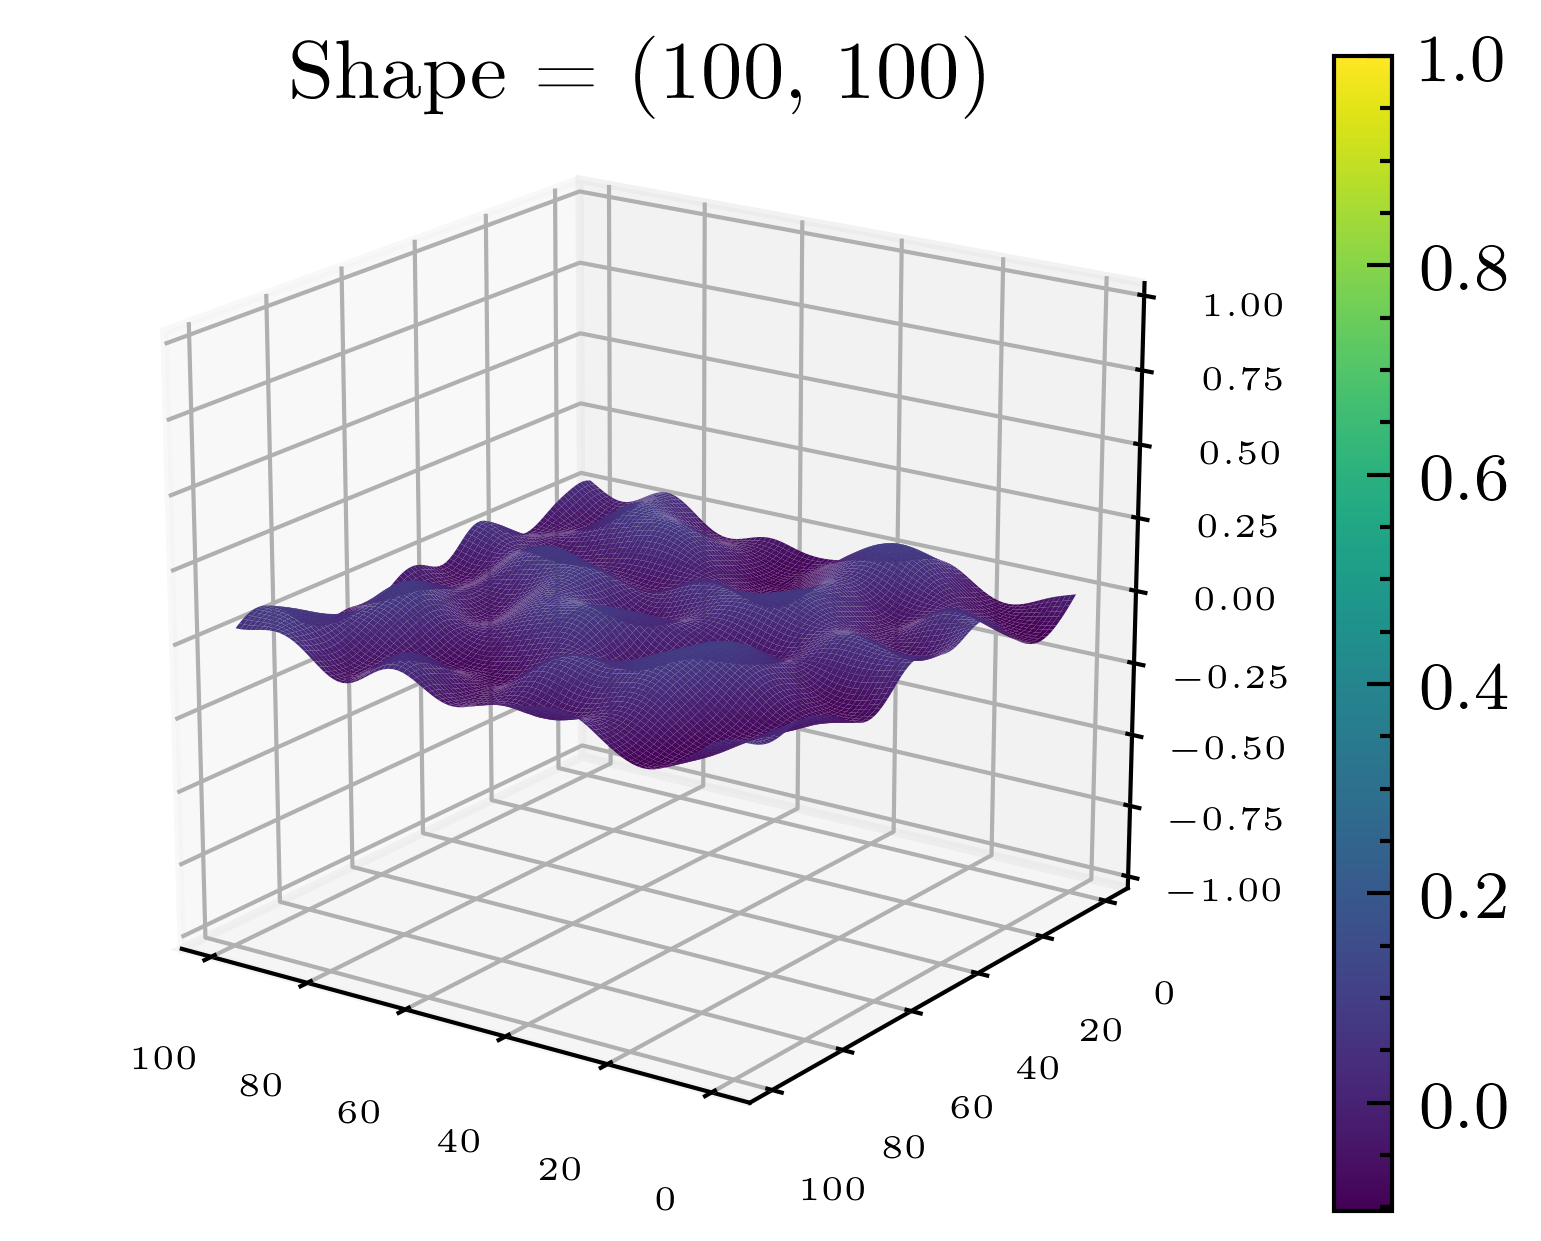
\includegraphics[width=\textwidth]{../img/data-aug/3d/simplex2.png}
            \caption{Data-aug}
            \end{subfigure}    
          \begin{subfigure}[b]{0.45\textwidth}
            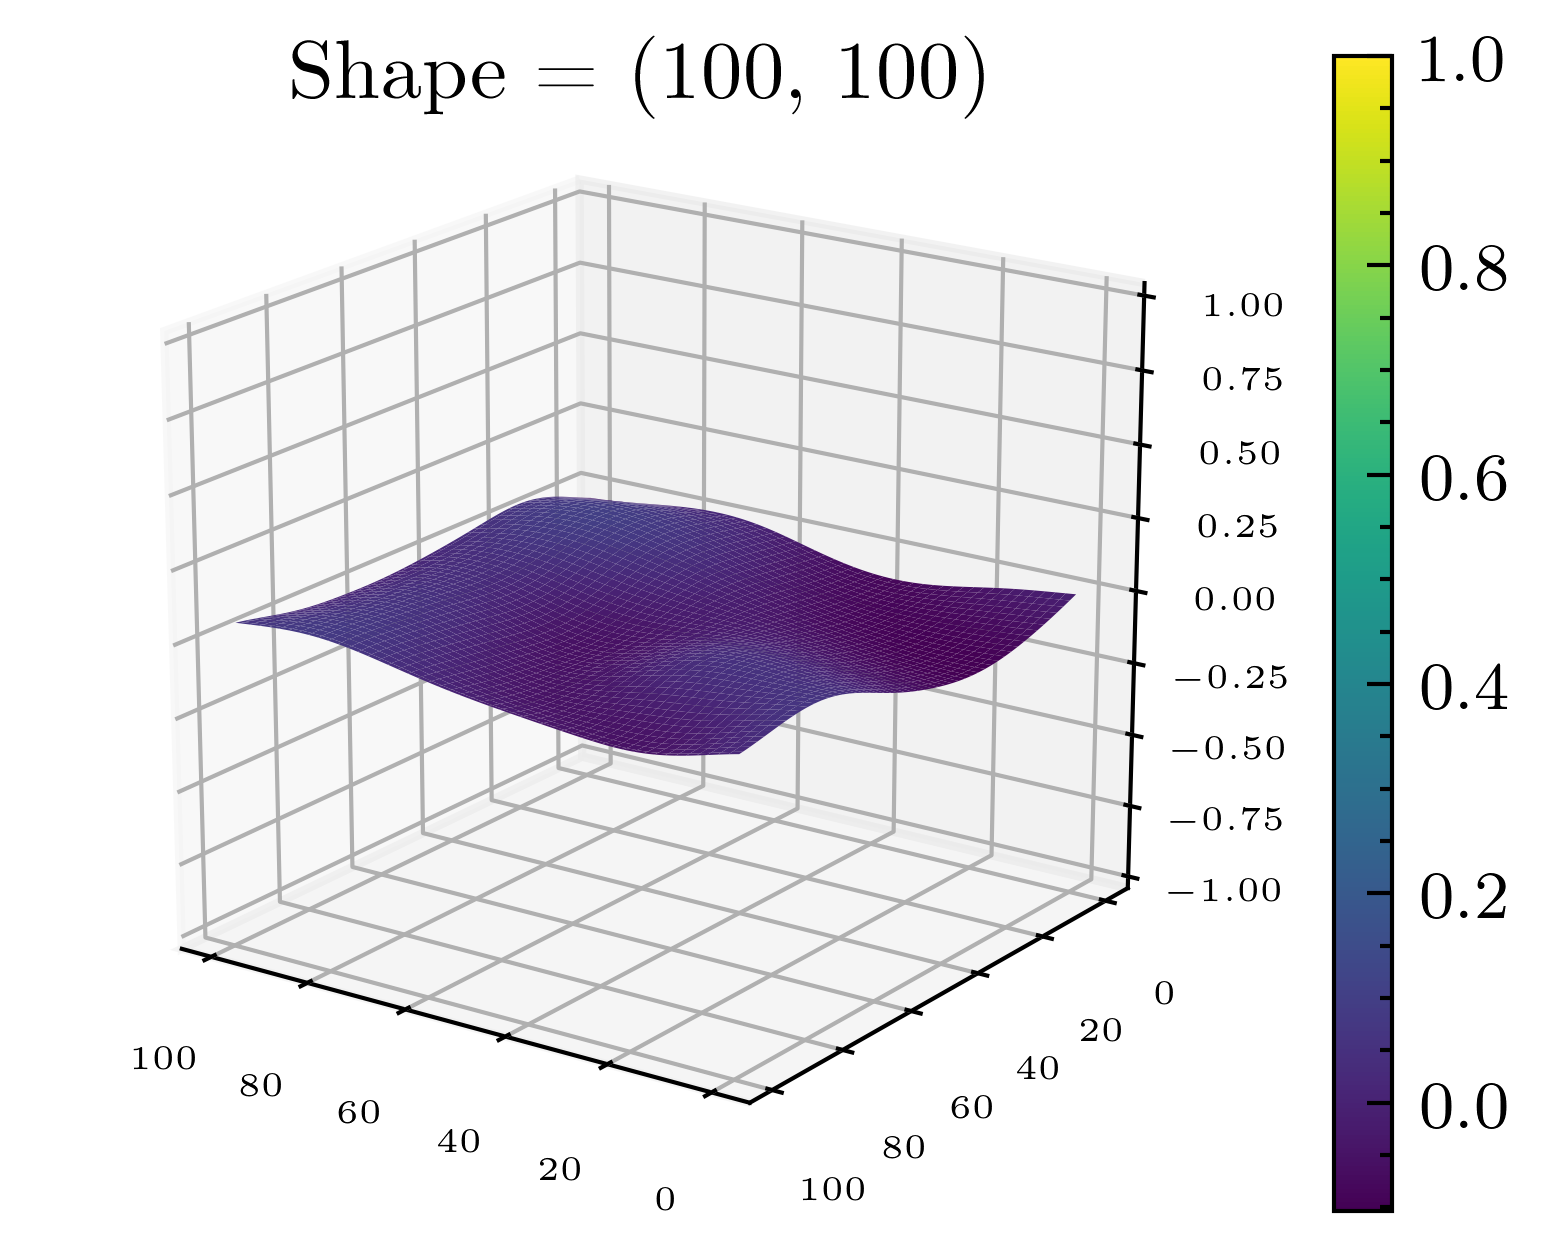
\includegraphics[width=\textwidth]{../img/data-aug/3d/simplex3.png}
            \caption{Features size = 30}
        \end{subfigure}    
        \begin{subfigure}[b]{0.45\textwidth}
            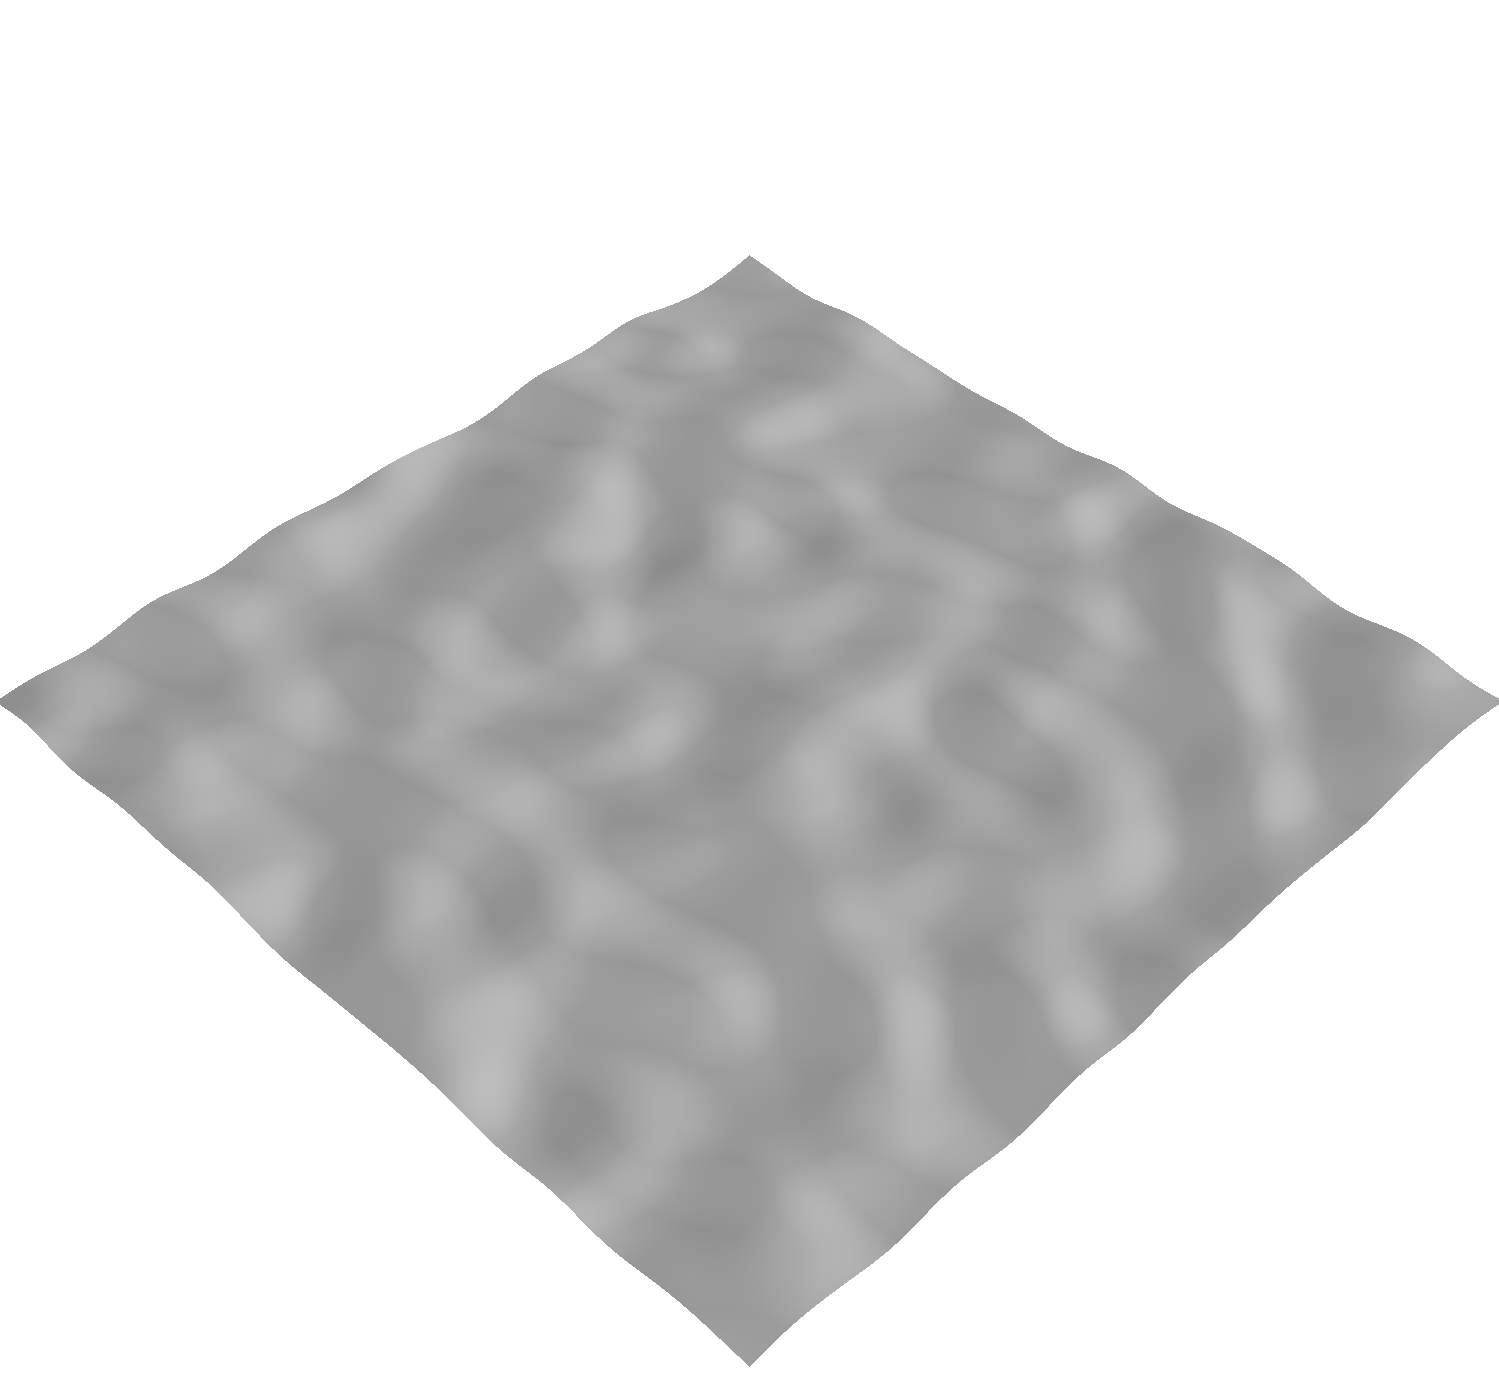
\includegraphics[width=\textwidth]{../img/data-aug/3d/simplex4.png}
            \caption{Features size = 40}
        \end{subfigure}    
    \label{fig: simplex-noise}
    \caption{Simplex Noise on flat ground}    
\end{figure}

The following images shows the tree data augmentation techniques used applied the input image.
\begin{figure}[H]
    \centering
        \begin{subfigure}[b]{0.45\textwidth}
            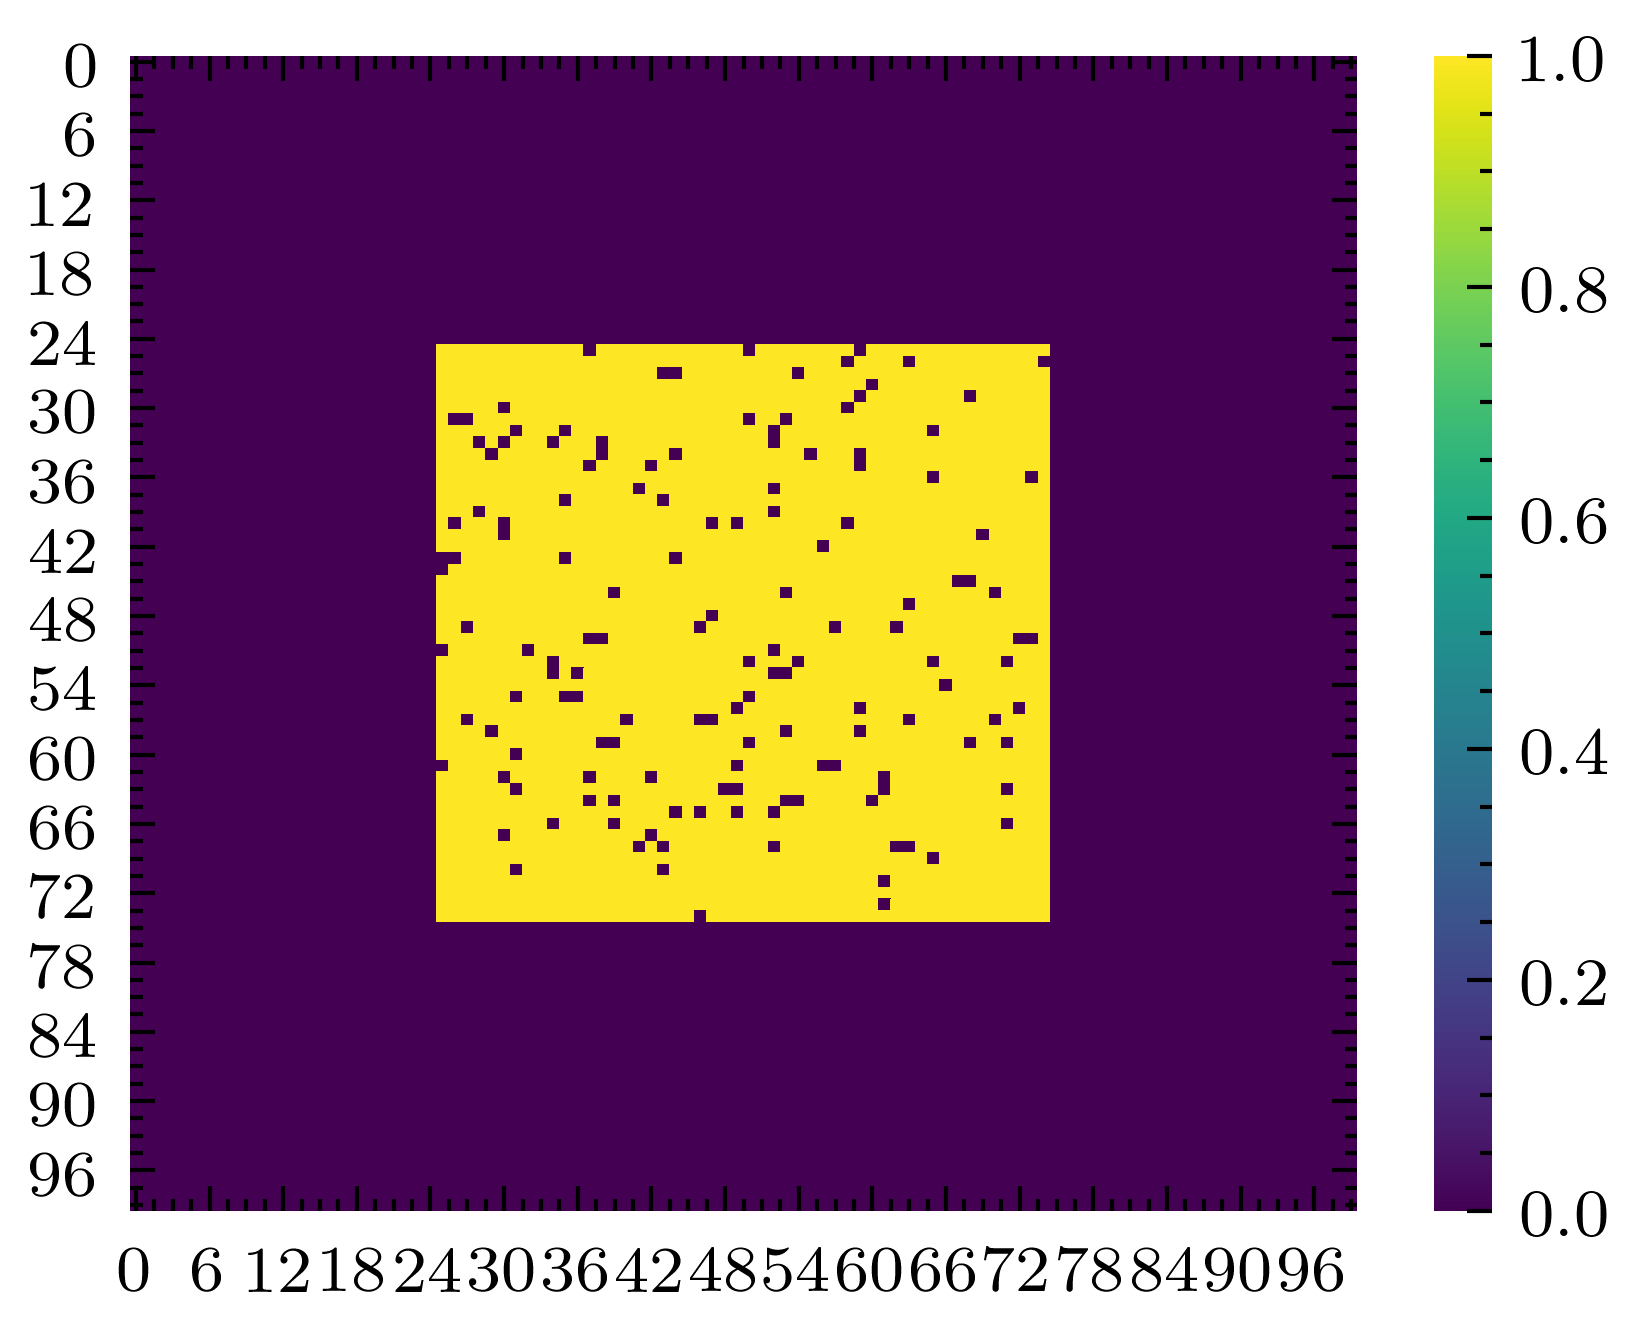
\includegraphics[width=\textwidth]{../img/data-aug/2d/center-dropout.png}
            \caption{Dropout}
        \end{subfigure}
        \begin{subfigure}[b]{0.45\linewidth}
            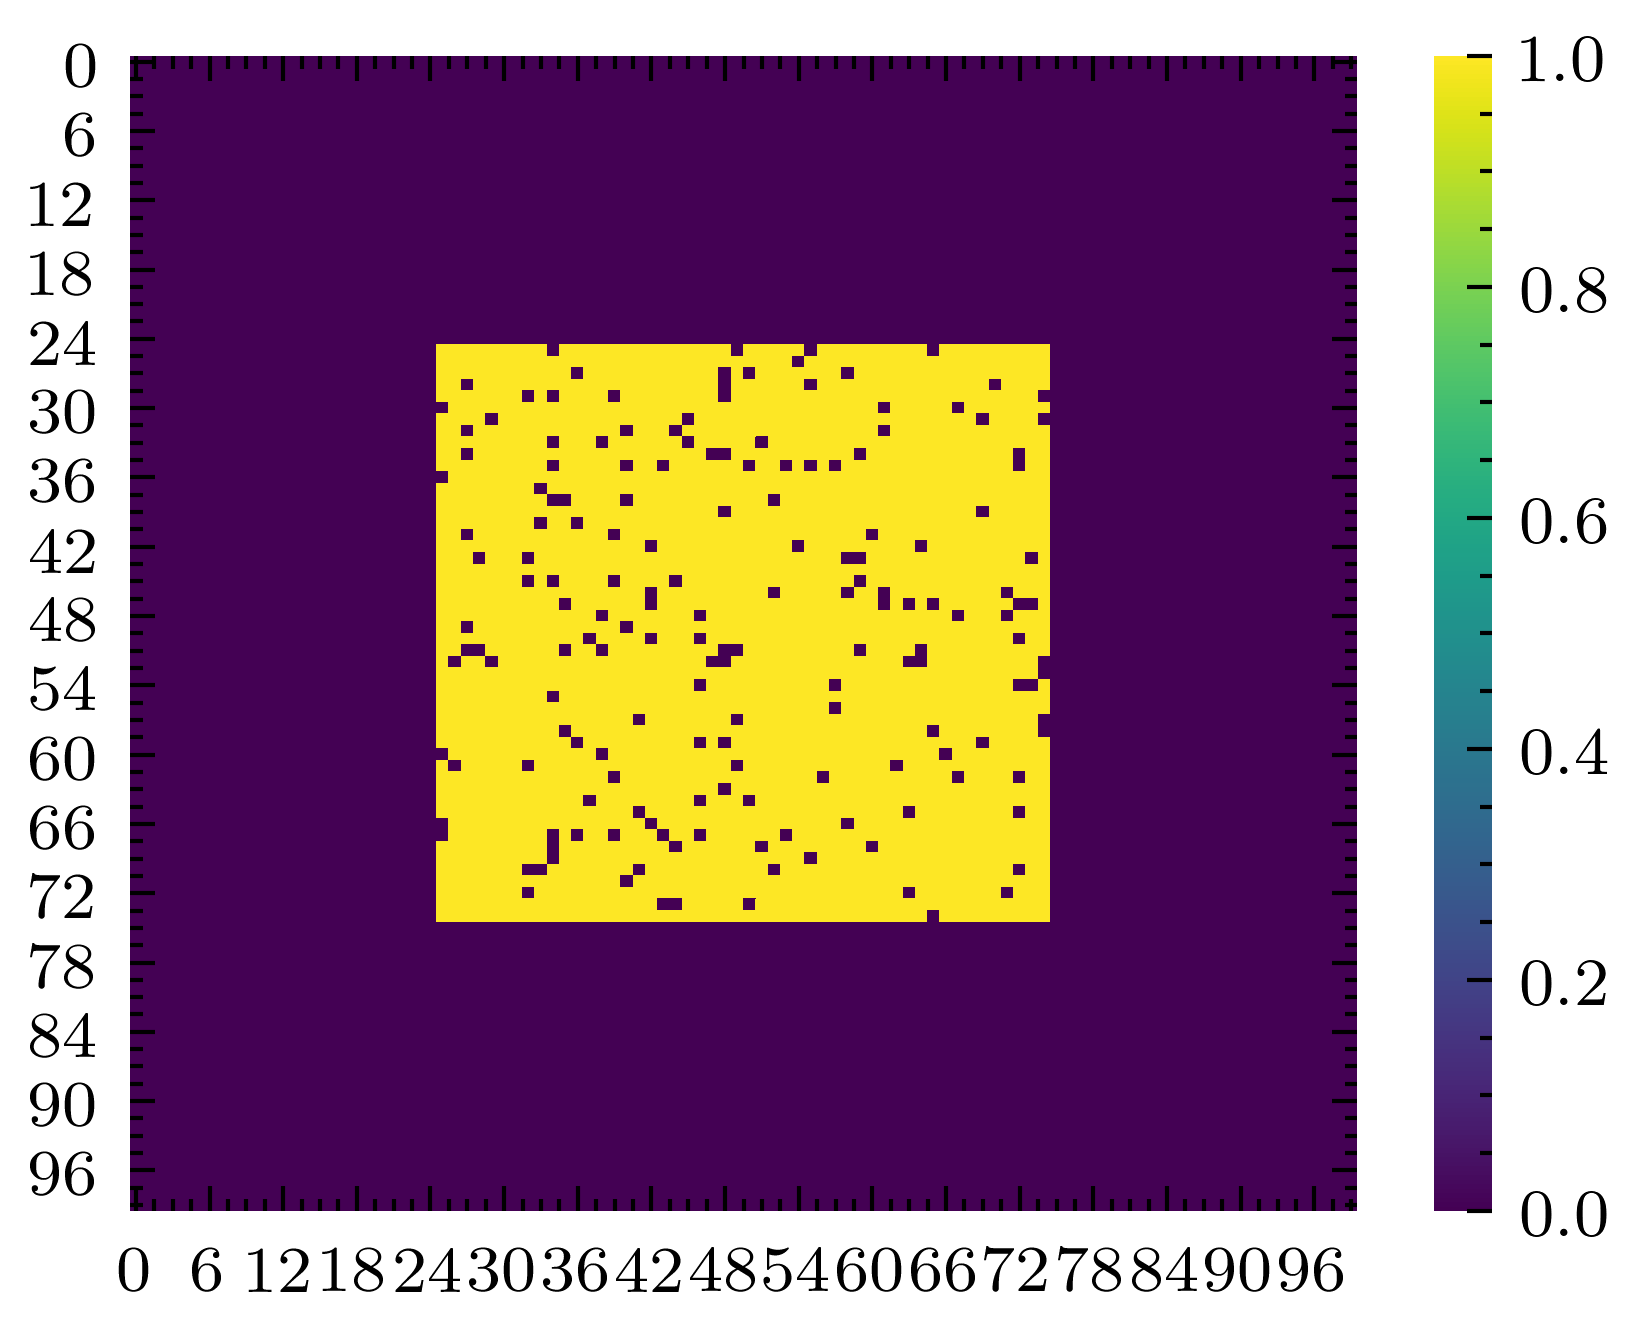
\includegraphics[width=\textwidth]{../img/data-aug/2d/center-coarse-dropout.png}
            \caption{Coarse Dropout}
            \end{subfigure}    

          \begin{subfigure}[b]{0.45\textwidth}
            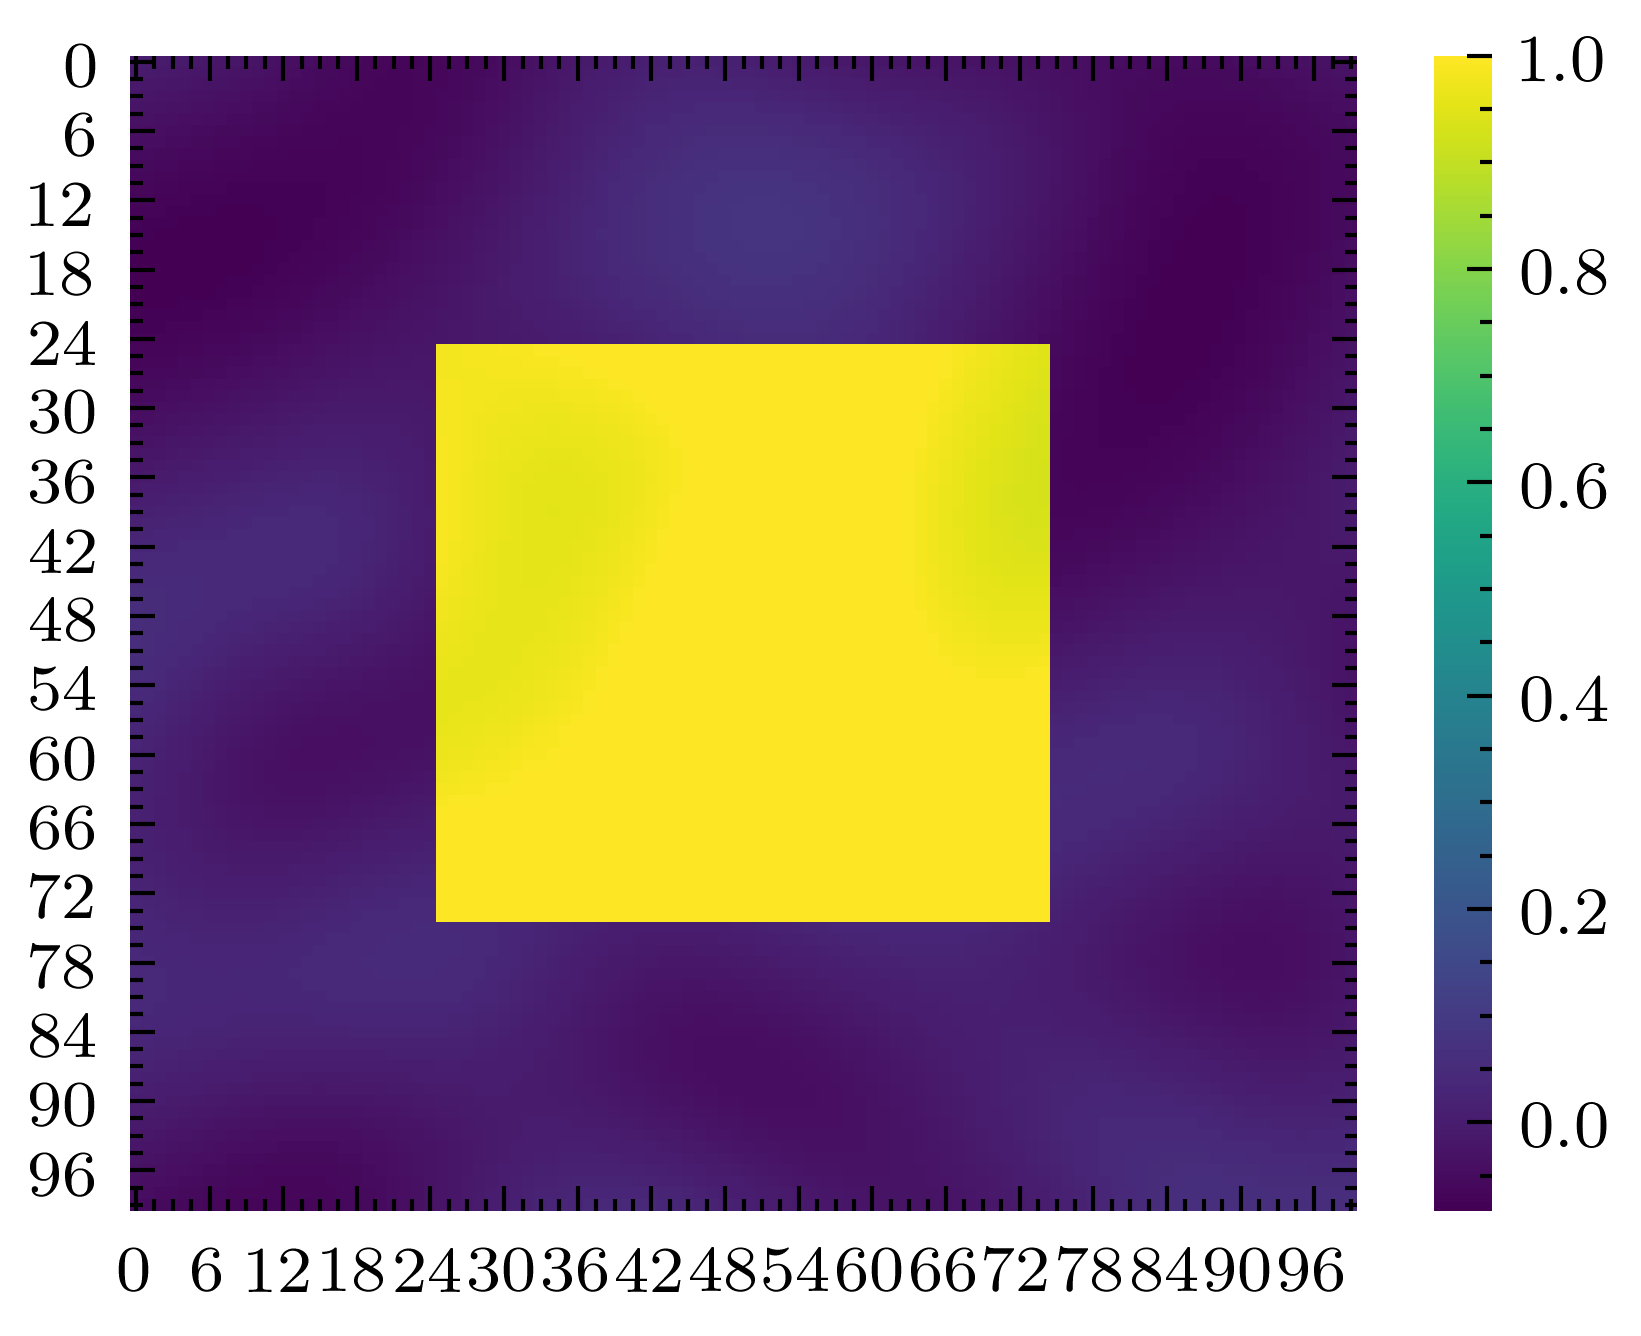
\includegraphics[width=\textwidth]{../img/data-aug/2d/center-simplex.png}
            \caption{Simplex Noise}

        \end{subfigure}    
        \begin{subfigure}[b]{0.45\textwidth}
            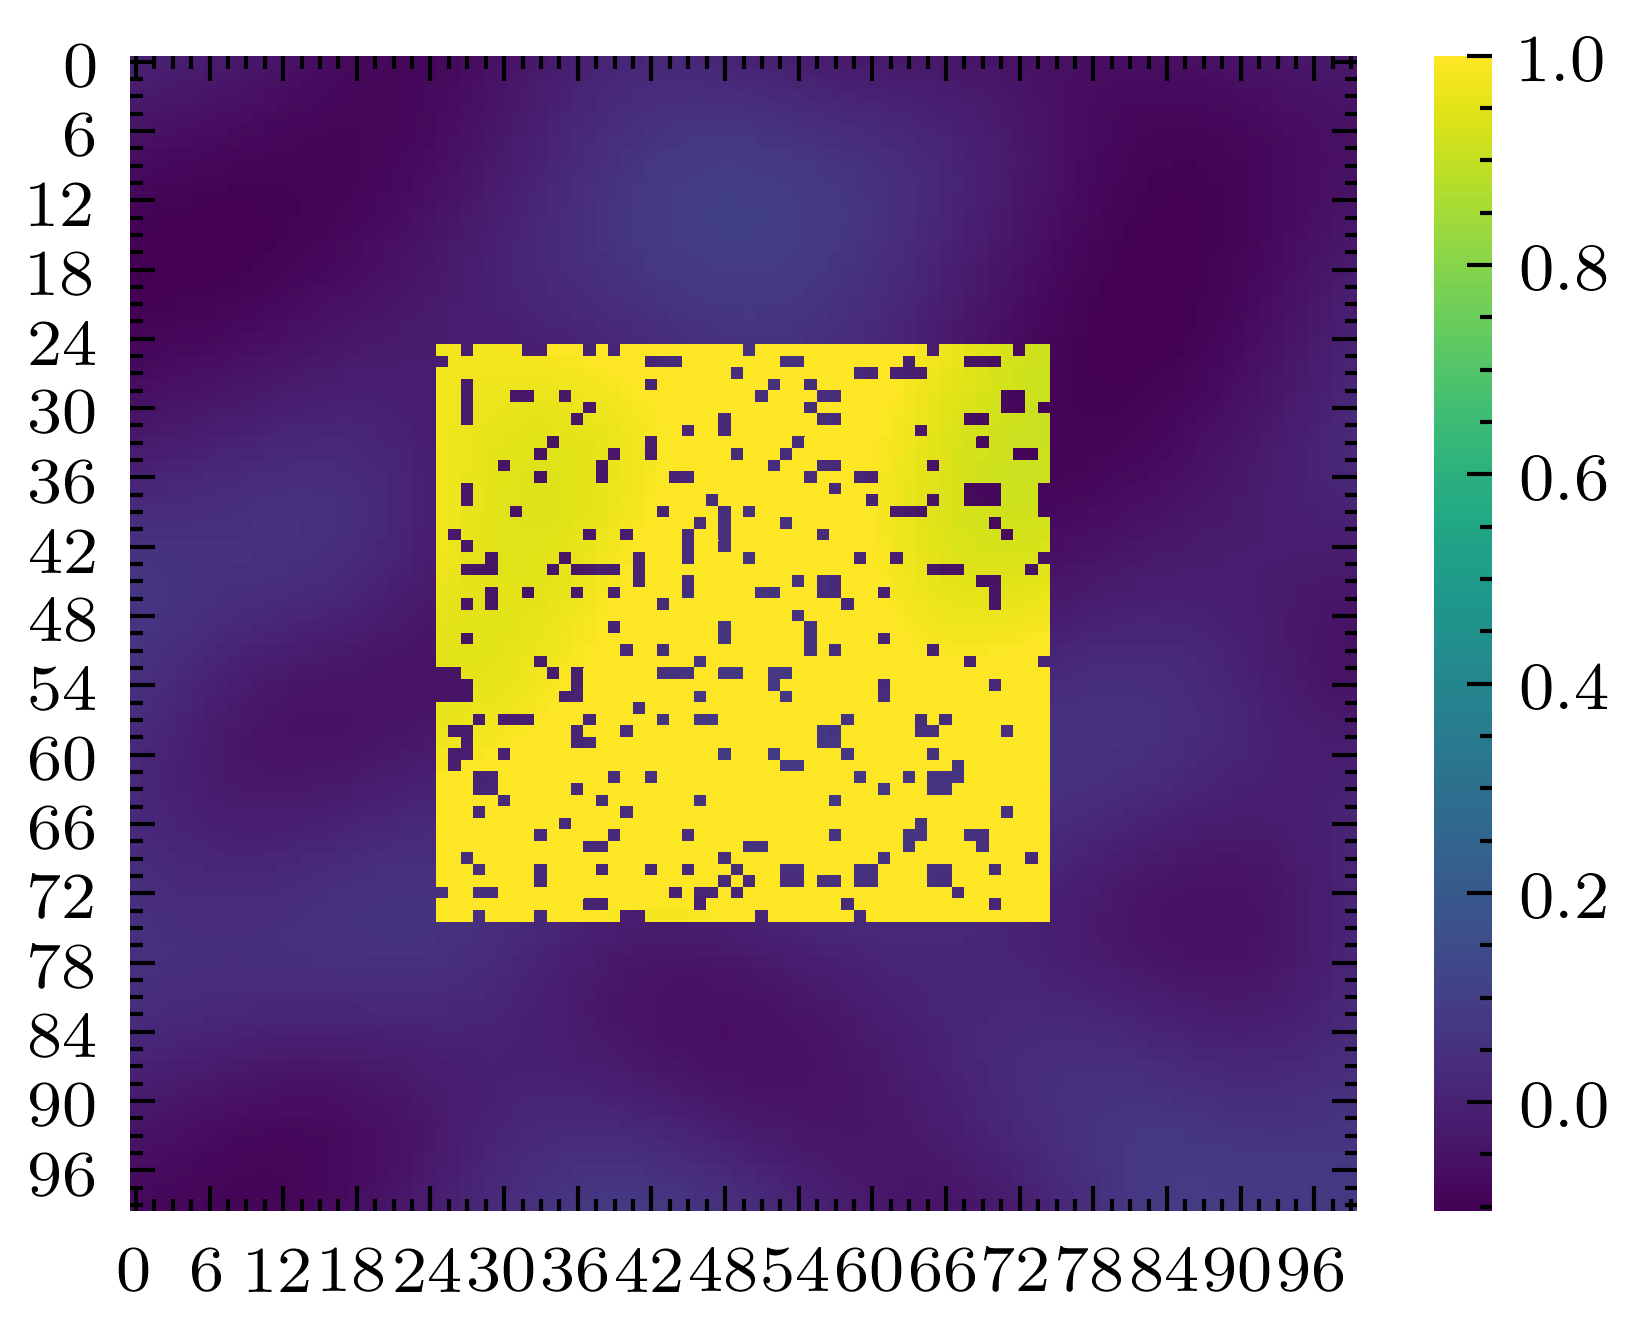
\includegraphics[width=\textwidth]{../img/data-aug/2d/center-aug.png}
            \caption{Final result}
        \end{subfigure}    
    \label{fig: square-patch-aug}
    \caption{Data augmentation}    
\end{figure}
It follows an other set of figures that shows the data augmentation we utilised on different inputs.

\begin{figure}[H]
    \centering
        \begin{subfigure}[b]{0.45\textwidth}
            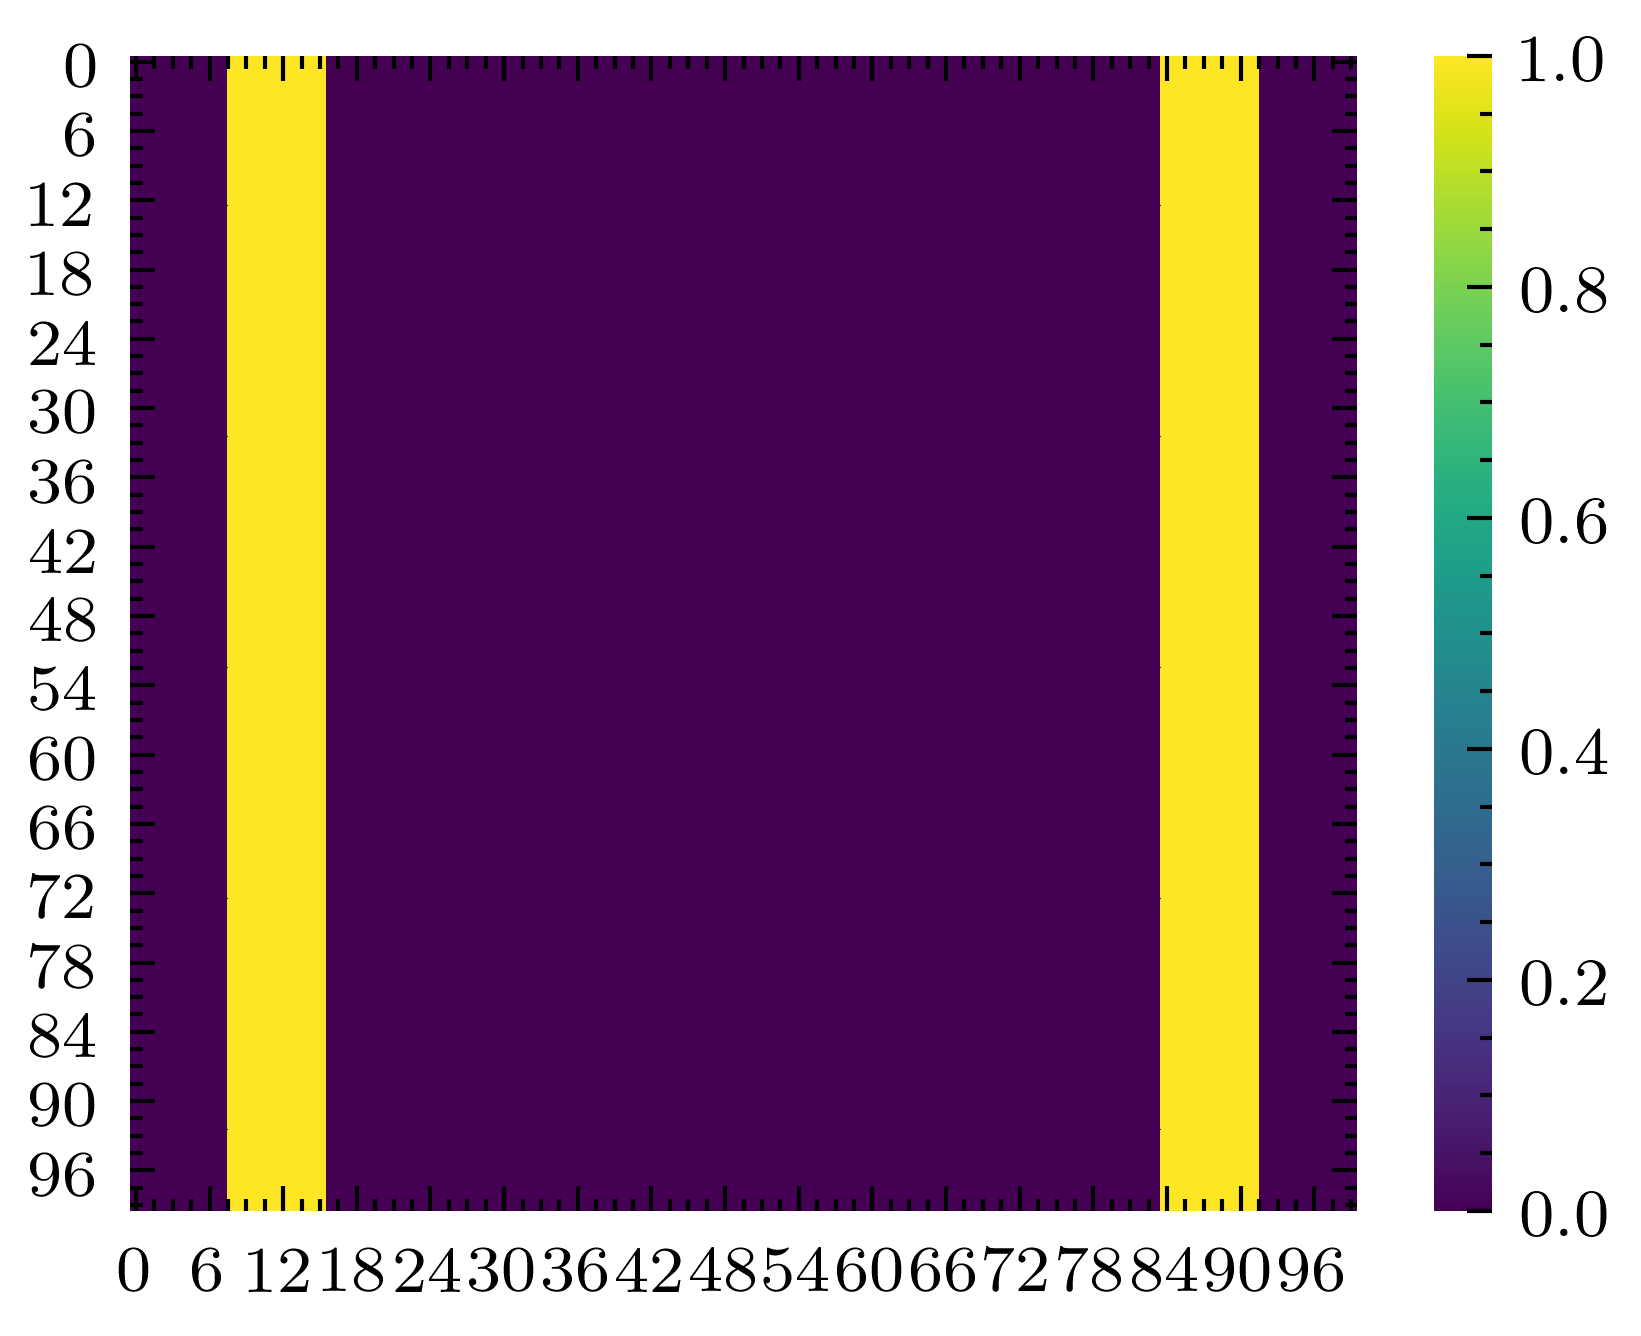
\includegraphics[width=\textwidth]{../img/data-aug/2d/wall.png}
            \caption{Walls}
        \end{subfigure}
        \begin{subfigure}[b]{0.45\linewidth}
            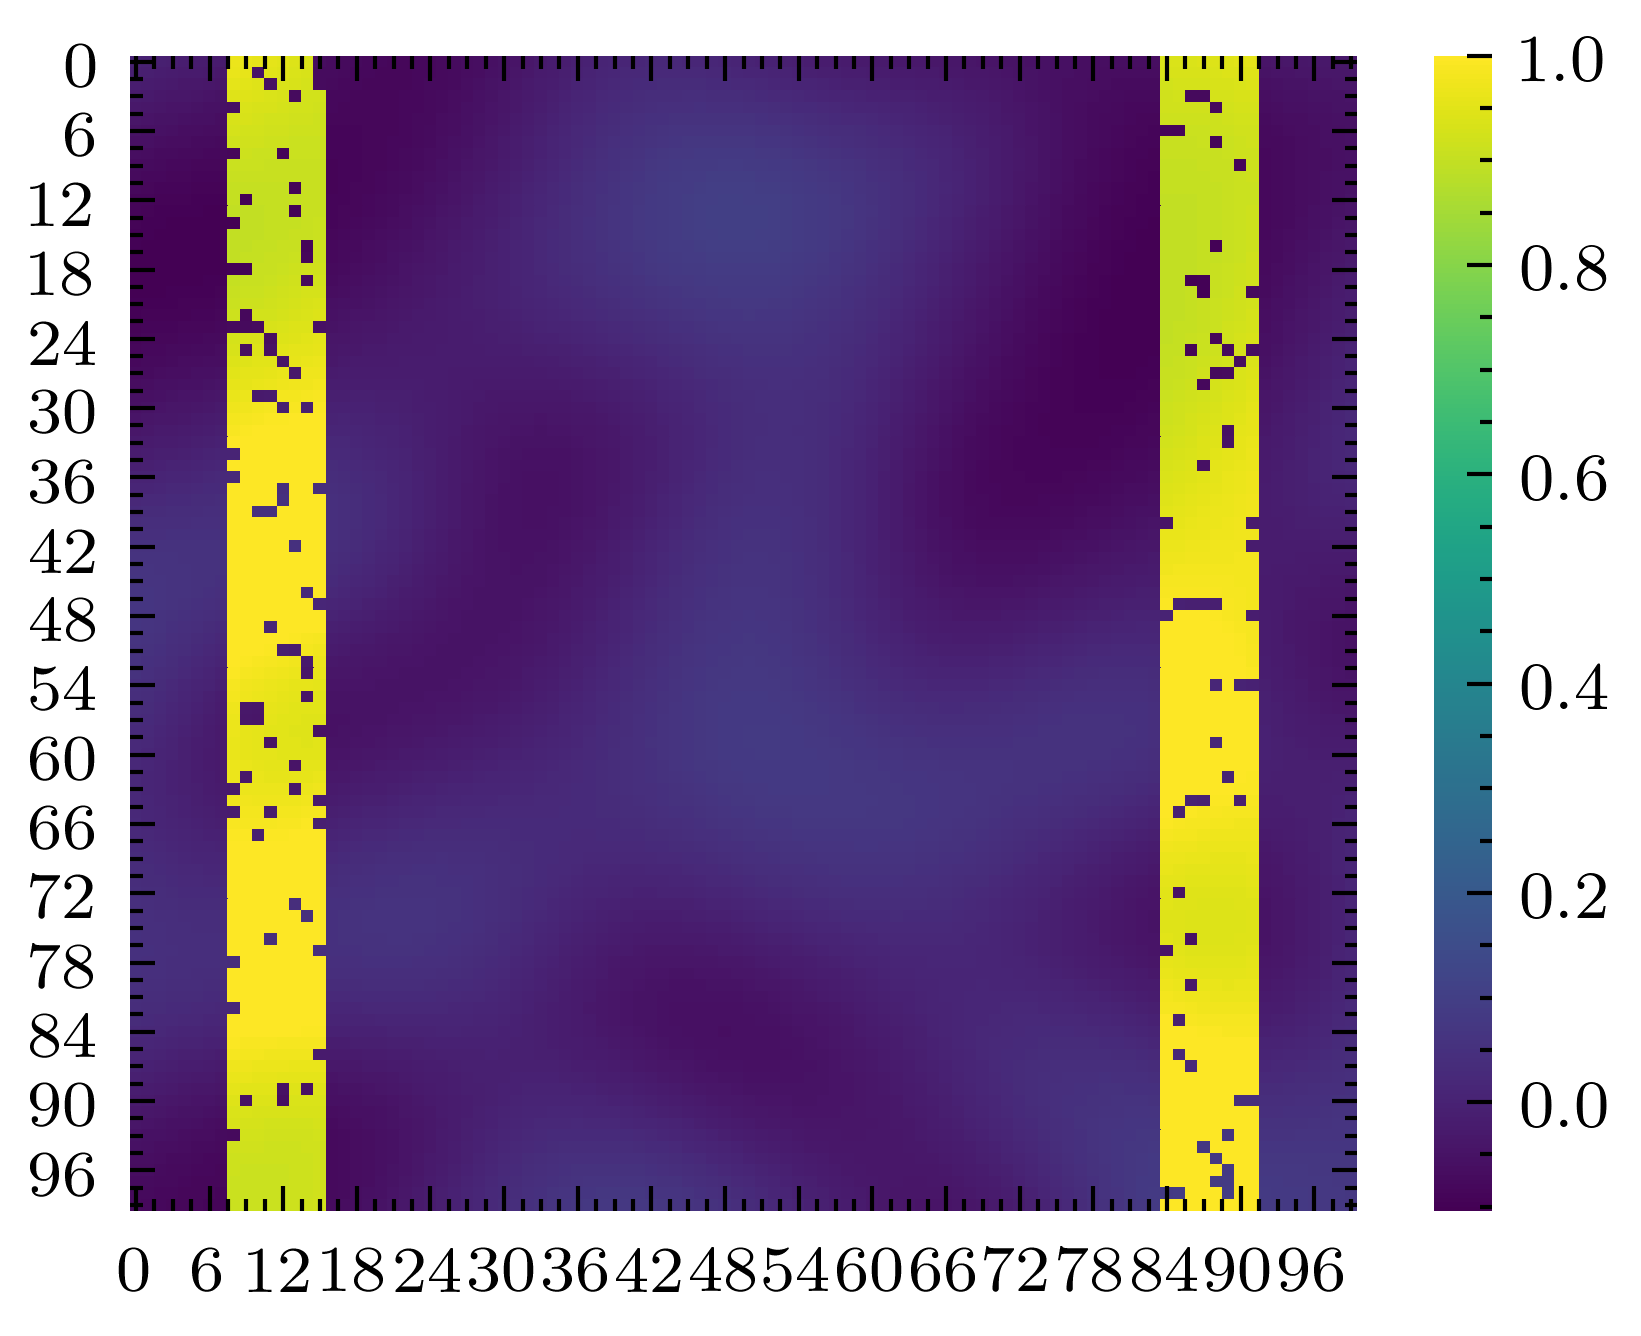
\includegraphics[width=\textwidth]{../img/data-aug/2d/wall-aug.png}
            \caption{Walls aug}
        \end{subfigure}    
        \begin{subfigure}[b]{0.45\textwidth}
            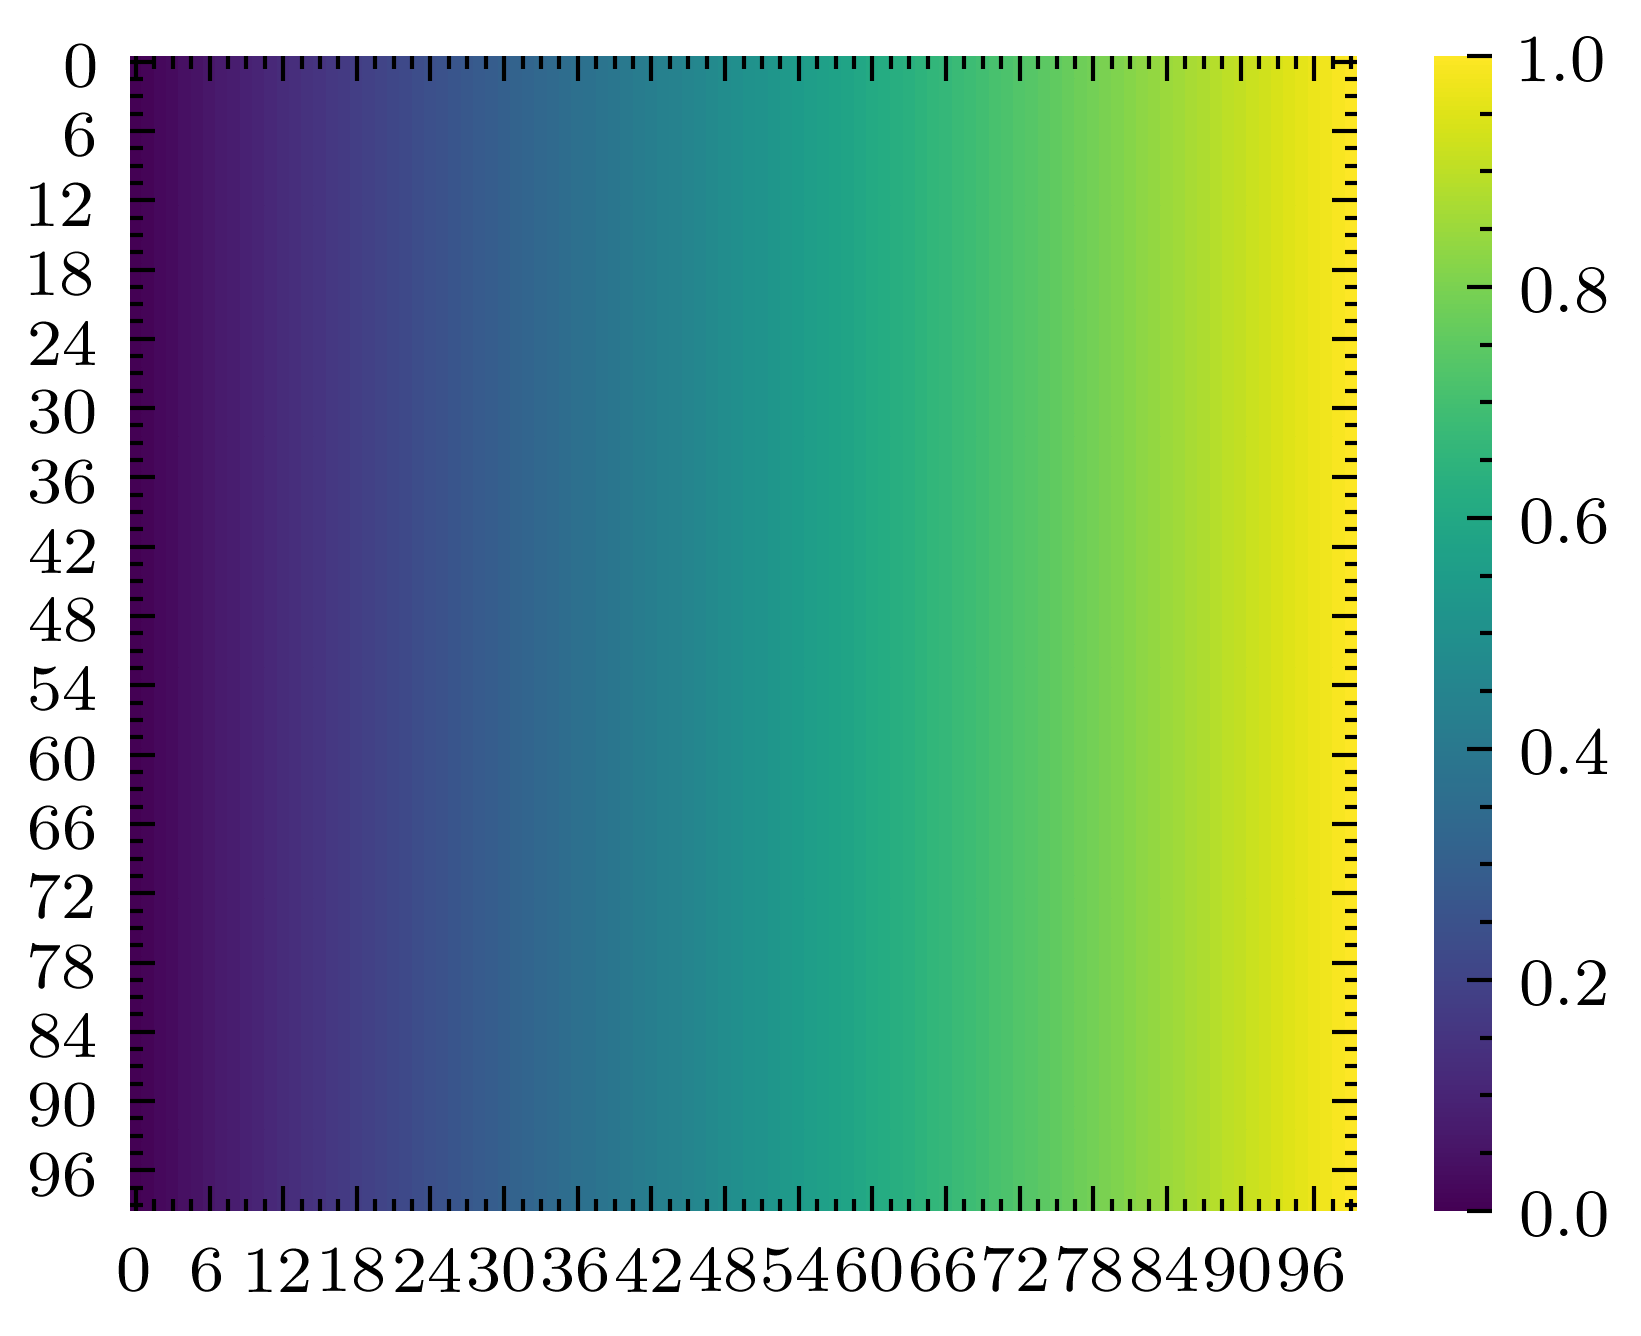
\includegraphics[width=\textwidth]{../img/data-aug/2d/ramp.png}
            \caption{Ramp}
        \end{subfigure}
        \begin{subfigure}[b]{0.45\linewidth}
            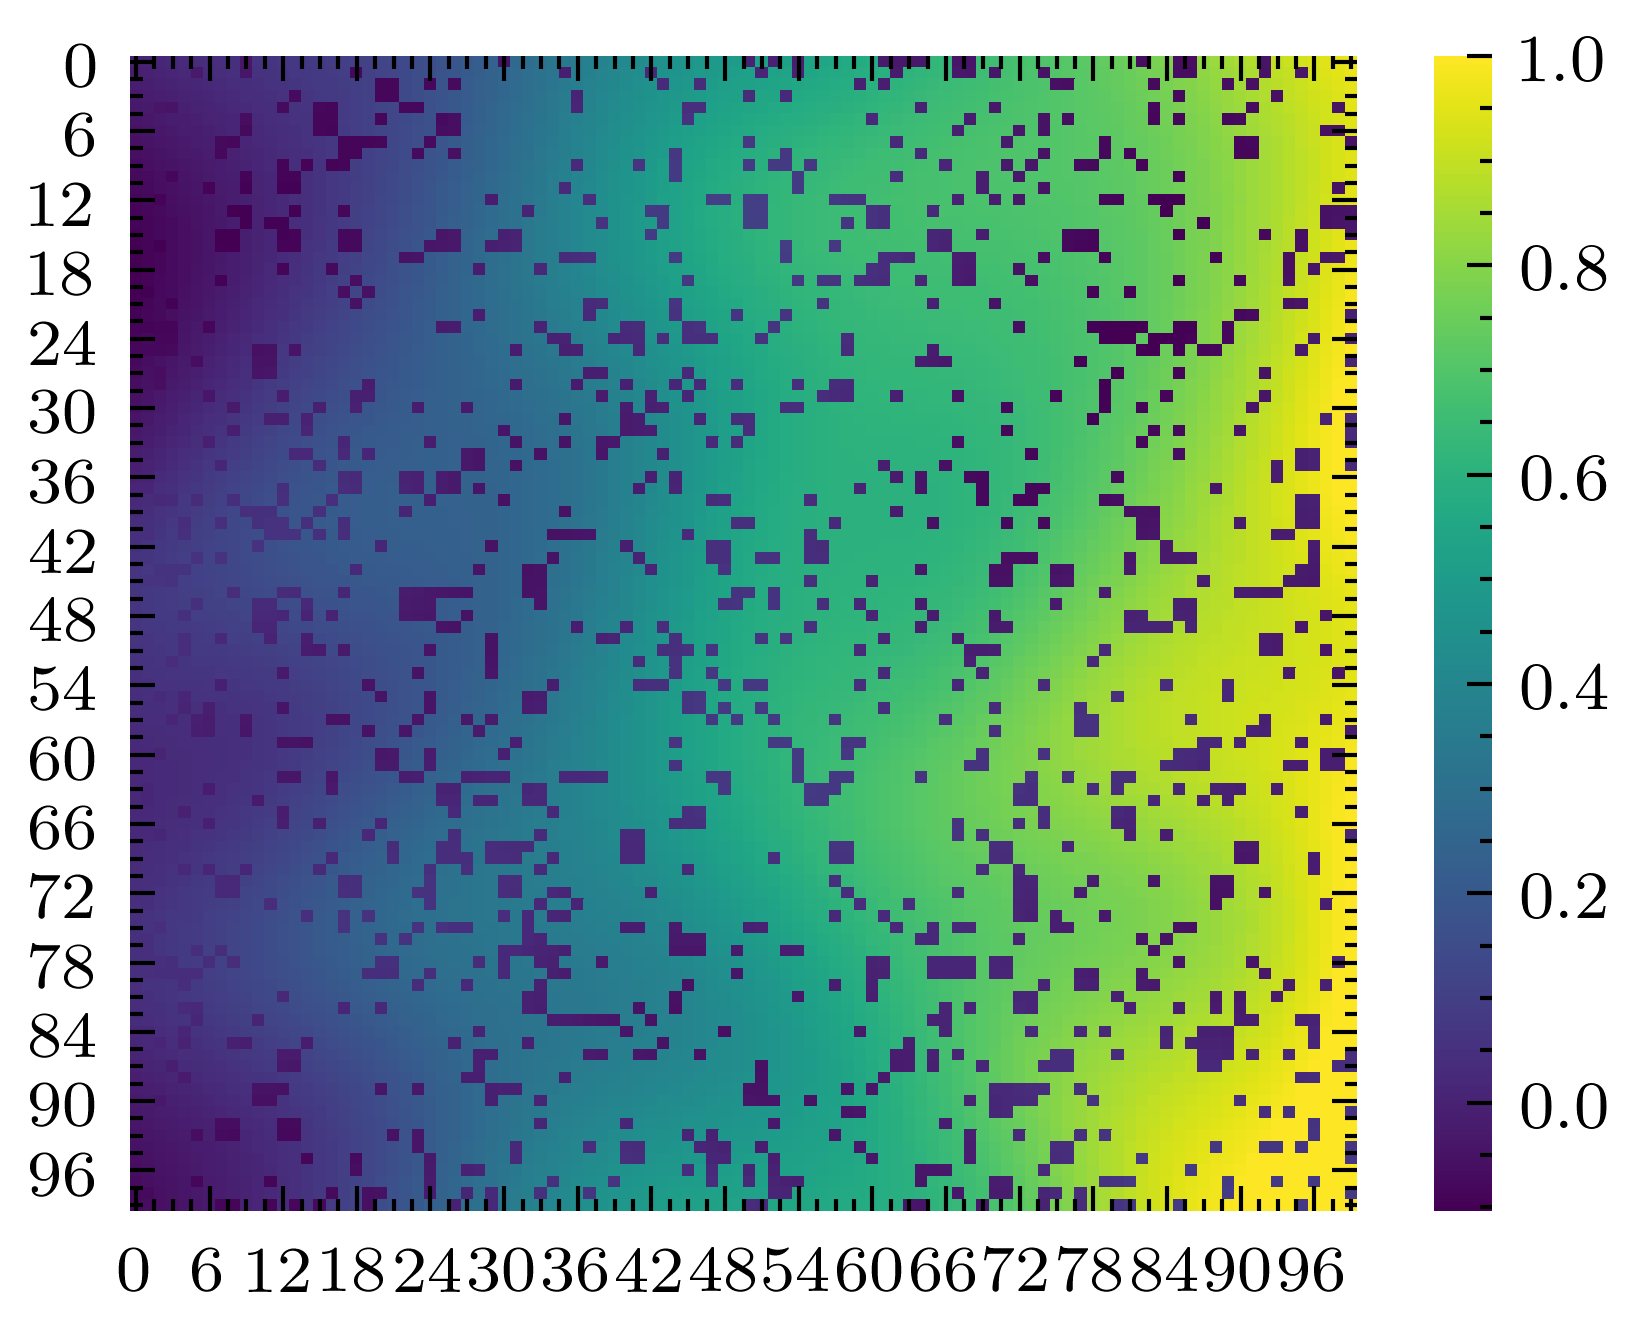
\includegraphics[width=\textwidth]{../img/data-aug/2d/ramp-aug.png}
            \caption{ramp aug}
        \end{subfigure}    
    \label{fig: others-aug}
    \caption{Wall}    
\end{figure}
\todo[inline]{add the parameters that we set}
In all the traning epochs, we apply data-augmentation to each input image $x$ with a probability of $0.8$. Dropout has a probability between $0.05$ and $0.1$. Coarse dropout with a probability of $0.02$ and $0.1$ with a size of the lower resolution image from which to sample the dropout between $0.6$ and $0.8$. Simplex noise with a feature size between $1$ and $50$ with a random scaling factor between $6$ and $10$. 
\end{document}